% Header %
% @author: Jan Lejnar
% options:
% thesis=B bachelor's thesis
% thesis=M master's thesis
% czech thesis in Czech language
% slovak thesis in Slovak language
% english thesis in English language
% hidelinks remove colour boxes around hyperlinks

\documentclass[thesis=M,czech]{FITthesis}[2019/12/23]

\usepackage[utf8]{inputenc} % LaTeX source encoded as UTF-8

\usepackage{graphicx} %graphics files inclusion
% \usepackage{amsmath} %advanced maths
% \usepackage{amssymb} %additional math symbols

\usepackage{dirtree} %directory tree visualisation
\usepackage{listings}
\usepackage{float} % \begin{figure}[''placement specifier'']
\usepackage{longtable}
\usepackage{color, colortbl}
\usepackage{hyperref}
\hypersetup{
    	colorlinks=false, % color frames in pdf
    	linkcolor=blue
} 
\definecolor{Blue}{rgb}{0.0, 0.75, 1.0}
\definecolor{Gray}{gray}{0.9}
\newcolumntype{g}{>{\columncolor{Gray}}p{0.20\textwidth}}
\newcommand{\lbparagraph}[1]{\paragraph{#1}\mbox{}\\} % paragraph with linebreak


\def\listingsfont{\ttfamily}
\lstset{
    extendedchars=true,
    literate=  
		 {á}{{\'a}}1
         {í}{{\'i}}1
         {é}{{\'e}}1
         {ý}{{\'y}}1
         {ú}{{\'u}}1
         {ó}{{\'o}}1
         {ě}{{\v{e}}}1
         {š}{{\v{s}}}1
         {č}{{\v{c}}}1
         {ř}{{\v{r}}}1
         {ž}{{\v{z}}}1
         {ď}{{\v{d}}}1
         {ť}{{\v{t}}}1
         {ň}{{\v{n}}}1                
         {ů}{{\r{u}}}1
         {Á}{{\'A}}1
         {Í}{{\'I}}1
         {É}{{\'E}}1
         {Ý}{{\'Y}}1
         {Ú}{{\'U}}1
         {Ó}{{\'O}}1
         {Ě}{{\v{E}}}1
         {Š}{{\v{S}}}1
         {Č}{{\v{C}}}1
         {Ř}{{\v{R}}}1
         {Ž}{{\v{Z}}}1
         {Ď}{{\v{D}}}1
         {Ť}{{\v{T}}}1
         {Ň}{{\v{N}}}1                
         {Ů}{{\r{U}}}1   
  ,
}
% % list of acronyms
% \usepackage[acronym,nonumberlist,toc,numberedsection=autolabel]{glossaries}
% \iflanguage{czech}{\renewcommand*{\acronymname}{Seznam pou{\v z}it{\' y}ch zkratek}}{}
% \makeglossaries

\newcommand{\tg}{\mathop{\mathrm{tg}}} %cesky tangens
\newcommand{\cotg}{\mathop{\mathrm{cotg}}} %cesky cotangens
\newenvironment{reusefigure}[2][htbp]
  {\addtocounter{figure}{-1}%
   \renewcommand{\theHfigure}{dupe-fig}% If you're using hyperref
   \renewcommand{\thefigure}{\ref{#2}}% Figure counter is \ref
   \renewcommand{\addcontentsline}[3]{}% Avoid placing figure in LoF
   \begin{figure}[#1]}
  {\end{figure}} % reuse figure

% Body %
\department{Katedra softwarového inženýrství}
\title{Vzorový dotazovací systém pro API existujícího informačního systému}
\authorGN{Jan} %(křestní) jméno (jména) autora
\authorFN{Lejnar} %příjmení autora
\authorWithDegrees{Bc. Jan Lejnar} %jméno autora včetně současných akademických titulů
\author{Jan Lejnar} %jméno autora bez akademických titulů
\supervisor{Ing. Jan Vrána, Ph.D.}
\acknowledgements{Mé poděkování patří v~první řadě Ing. Janu Vránovi, Ph.D. za nabídnutí možnosti práce na tomto projektu, ve mě vloženou důvěru, cenné rady a věcné připomínky, zejména v~úvodní části sběru požadavků a později při návrhu architektury. Děkuji Tomášovi Novákovi, bez kterého by aplikace neměla grafickou podobu. Dále velmi děkuji Tomášovi Traplovi za vstřícnost při konzultacích analytické části práce. V~neposlední řadě děkuji Ladislavovi Zámečníkovi, za jeho entuziazmus při předávání zpětné vazby na potenciální problémy v~implementaci.}
\abstractCS{Tato práce se zabývá návrhem a vývojem vzorového dotazovacího systému, který poskytne koncovým uživatelům příjemnou formou webového rozhraní možnost kladení dotazů do již existujícího informačního systému, který pro dotazování jinak poskytuje pouze složité API rozhraní.
Navržený systém bude sloužit buď k~přímému použití menším subjektům, které samy nemají potřebné zdroje pro vybudování vlastního řešení, nebo jako vzorové řešení větším subjektům, které si budou moci, na základě tohoto vzoru, vybudovat vlastní dotazovací systém.
Aplikace byla úspěšně vytvořena dle běžného softwarového procesu, od sběru uživatelských požadavků, přes analýzu problematiky, návrh řešení, jeho implementaci, až po jeho testování a~dokumentaci.
Požadavky na systém byly splněny. Aplikace umožňuje sestavení různých variant typických dotazů do dotazovacího API a prezentaci získaných výsledků prostřednictvím webového rozhraní.}
\abstractEN{This thesis targets designing a model query system, which will provide to end-users a web interface to query an existing information system, which otherwise provides only a complex API for querying.
The resulting product is intended mainly for smaller organizations that do not have the necessary resources to build their own solution, or as a model solution for larger organizations, which will be able to create their own query system based on this model.
The application was successfully created according to the standard software process, from requirement gathering, through analysis, design, implementation, to testing, and documentation. 
All system requirements have been met. The application enables its users to build various types of queries, send them to the API and represent obtained results via a web interface.}
\placeForDeclarationOfAuthenticity{V~Praze}
\declarationOfAuthenticityOption{6} %volba Prohlášení (číslo 1-6)
\keywordsCS{dotazovací systém, uživatelské rozhraní, sestavování dotazů, transformace dotazů, prezentace výsledků\newpage}
\keywordsEN{query system, user interface, queries building, query transformation, presentation of results}
% \website{http://site.example/thesis} %volitelná URL práce, objeví se v tiráži - úplně odstraňte, nemáte-li URL práce

\begin{document}
% \newacronym{CVUT}{{\v C}VUT}{{\v C}esk{\' e} vysok{\' e} u{\v c}en{\' i} technick{\' e} v Praze}
% \newacronym{FIT}{FIT}{Fakulta informa{\v c}n{\' i}ch technologi{\' i}}

\begin{introduction}
Zadavatel si nepřál zveřejnit některé údaje z~této práce, proto muselo dojít k~anonymizaci těchto údajů, refactoringu kódu a zobecnění zadání práce, aby neexistovala žádná spojitost mezi produktem této práce a skutečným informačním systémem. To schválil vedoucí katedry softwarového inženýrství Ing. Michal Valenta, Ph.D.

V~zadání zmíněný existující informační systém budu dále označovat pod anonymizovaným termínem IS~AAA. Některé ostatní pojmy mohly být rovněž upraveny, pokud jejich přesný název nebyl podstatný pro účel diplomové práce.

IS~AAA (tj. Informační systém AAA) je rozsáhlá databáze, která umožňuje příslušným organizacím využívat údaje, které byly do databáze zaneseny. Zadavatel zastřešuje více organizací, které potřebují s~IS~AAA komunikovat.

Vzhledem k~vzrůstajícímu počtu organizací, které si musely vytvořit vlastní dotazovací aplikaci, bylo potřeba vytvořit vzorový dotazovací systém, který nabídne webové uživatelské rozhraní pro zasílání typických dotazů do systému IS~AAA. Systém bude určen zejména menším organizacím, které dosud nemají vlastní dotazovací systém a plánují zasílat dotazy do IS~AAA.

Výsledným produktem bude opakovatelně využitelná (\textit{reusable}) aplikace, která bude sloužit jako produkčně užívaná aplikace pro organizace s~menší skupinou uživatelů (3 -- 5 uživatelů) nebo jako vzorové řešení, tvořící základ pro další rozvoj, pokud organizace usoudí, že potřebuje doplnit nějakou vlastní funkcionalitu do vzorového dotazovacího systému (dále také pod označením Q-systém).

Z~tohoto důvodu bude systém založen na otevřených technologiích. Vyvinutý kód bude předán do vlastnictví zadavatele. Hlavním přínosem pro zadavatele bude omezení nevhodného používání nabízených služeb IS~AAA a umožnění pokládání dotazů koncovými uživateli.

\newpage
Toto téma jsem si vybral, protože to byla výjimečná příležitost projít si celým softwarovým procesem projektu, který má vzniknout \uv{na zelené louce} a který má potenciál každodenního reálného využití.
\end{introduction}

\chapter{Cíl práce}
Cílem této práce je navrhnout po softwarově-inženýrské stránce vzorový dotazovací systém, který nabídne webové uživatelské rozhraní pro zasílání typických dotazů (na osoby, vozidla, atd.) do Informačního systému AAA.

Pro dosažení tohoto cíle je potřeba splnit následující úkoly:
\begin{enumerate}
	\item Sběr požadavků a analytický popis zkoumané domény 
	\item Popis scénářů případů použití a návrh systému
	\item Vytvoření uživatelské dokumentace
	\item Implementace funkčního prototypu backendové části aplikace
\end{enumerate}

Z~důvodu omezení rozsahu běžné pracnosti na diplomovou práci se nepředpokládá odevzdání finální aplikace, pouze prototyp. Práce nezavazuje k~návrhu ani tvorbě frontendové části aplikace.

\chapter{Analýza}
\label{Analyza}
\section{Seznámení s~kontextem}
Na následujícím obrázku je naznačené základní komunikační schéma.
Produktem této práce je žlutě vyznačený vzorový dotazovací systém s~názvem Q-systém.

V~úvodu byl zmíněn systém IS~AAA. Tento název zahrnuje systém IS~AAAA a centrální systém IS~AAAB, který teprve přistupuje do databáze. 

IS~AAAA je technickým prostředníkem mezi Q-systémem a centrálním systémem IS~AAAB. IS~AAAA po přijetí dotazu nejprve provede kontrolu správnosti. Následně probíhá překlad číselníkových hodnot ze standardu zadavatele do standardu IS~AAA -- zdrojový text je zaměněn za text cílový (například \uv{červená} je nahrazena odpovídajícím kódem \uv{XXXX.YY}). Teprve nakonec je dotaz přeposlán do IS~AAAB. \cite{ICT}

\begin{figure}[H]
  \centering
  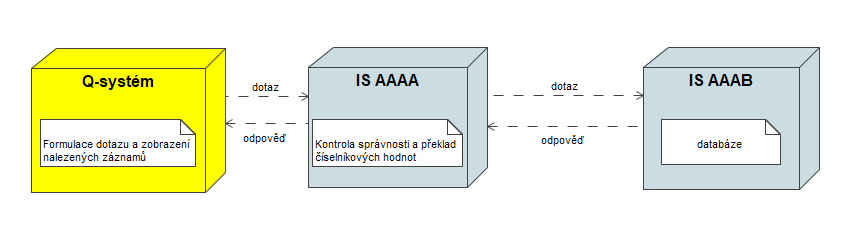
\includegraphics[width=\textwidth]{res/design/Základní komunikační schéma.png}
  \caption{Základní komunikační schéma}
  \label{fig:Základní komunikační schéma}
\end{figure}

\newpage
Vyvíjený vzorový dotazovací systém pro zadavatele bude komunikovat se systémem IS~AAAA. Poptávka po vytvoření vzorového dotazovacího systému vznikla, protože rozhraní systému IS~AAAA:
\begin{enumerate}
	\item je poměrně složité
	\item není volně dostupné a je potřeba jej zpřístupnit také dalším organizacím
\end{enumerate}

IS~AAAA nabízí opravdu bohaté rozhraní pro pokládání dotazů. Je možné se dotazovat například na tyto typy entit: \cite{Queries}
\begin{itemize}
	\item osoba
	\item vozidlo
	\item zboží
	\item skladová položka
	\item smlouva
	\item subjekt
	\item vztah
	\item transakce
	\item ekonomická jednotka
	\item opatření
	\item dodávka
\end{itemize}

\newpage
Vystavené rozhraní IS~AAAA se jmenuje \textit{Plné rozhraní}. Pro komunikaci používá webové služby nad protokolem SOAP. Zprávy mají XML formát.
Na toto rozhraní lze zasílat tyto typy dotazů: \cite{i1}
\begin{enumerate}
	\item Základní dotazy -- jejich cílem je zjištění, zda v~IS~AAAA existují, nebo neexistují záznamy odpovídající zadaným vyhledávacím atributům. Systém pak vrací seznam identifikátorů nalezených záznamů a jejich základní textové údaje. Vyhledávacím atributem může být jeden nebo více atributů zájmového objektu, např. jméno a datum narození u~osoby, nebo např. značka u~vozidla, barva a typ motoru, nebo jiné možné kombinace.
		\begin{enumerate}
			\item \textit{Základní dotaz} -- na základě jednoduchého dotazu v~určené struktuře vrací volajícímu systému seznam záznamů v~IS~AAAA, které odpovídají položenému dotazu, se základními informacemi o~předmětu záznamu
			\item \textit{SQL dotaz} -- dotaz je formulovaný jazykem SQL a umožňuje tak sestavit komplexnější dotaz mimo standardní strukturu
		\end{enumerate}
	\item Doplňkové dotazy -- jejich cílem je získání dalších rozšiřujících informací o~známém záznamu. Systém vrací další určené údaje tohoto konkrétního záznamu. Záznam je jednoznačně určen svým identifikátorem \texttt{AAA\_ID}, který byl získán např. základním dotazem.
		\begin{enumerate}
			\item \textit{Doplňující dotaz} -- načte doplňující textové údaje k~záznamu
			\item \textit{Načtení vazeb} -- načte vazby záznamu
			\item \textit{Načtení příloh} -- načte přílohy záznamu: fotografie apod.
		\end{enumerate}
\end{enumerate}

IS~AAAA vystavuje také rozhraní \textit{Zjednodušené rozhraní}, na jehož implementaci jsem se podstatnou měrou podílel předtím, než přišel požadavek na vytvoření Q-systému. Jedná se o~klon rozhraní \textit{Plné rozhraní}, s~několika rozdíly: \cite{i2}
	\begin{itemize}
		\item Vzniklo spíše pro externí organizace, aby nebylo tolik zatěžováno rozhraní \textit{Plné rozhraní}.
		\item Umožňuje omezit četnost použití služby pro určitou organizaci (QoS).
		\item Odpovídá pouze na dotazy typu \textit{Základní dotaz}.
		\item Poskytuje možnost omezit obsah odpovědi pro určitou organizaci, příkladem může být zakrytí nalezených záznamů v~odpovědi od IS~AAAB, které byly vloženy konkrétní organizací.
	\end{itemize}
	
\section{Organizační role}
V~této kapitole je uveden seznam typů pracovníků (tj. organizačních rolí), kteří budou popisovaný systém používat.

Ve fázi návrhu aplikačního vybavení budou některé organizační role přetransformovány do rolí uživatelů informačního systému.

\begin{table}[H]
	\centering
	\begin{tabular}{|p{0.20\textwidth}|p{0.80\textwidth}|}
		\hline
  		{\textbf{Typ \mbox{pracovníka}}} & {\textbf{Popis}} \\	
  		\hline \hline
  		Dotazovatel & Dotazovatel je uživatel pokládající dotazy do IS~AAAA.  \\ \hline
		Administrátor & Uživatel, který kromě posílání dotazů může změnit konfiguraci Q-systému, například nahraje nové číselníky, zvolí preferované rozhraní pro pokládání dotazů nebo definuje, jaké role mají povoleno pokládat dotazy určitého typu, s~určitým modifikátorem dotazu a na určité typy entit.  \\ \hline
	\end{tabular}
 	\caption{Seznam typů pracovníků s~aplikací}
\label{tab:Seznam typů pracovníků s~aplikací}
\end{table}

\section{Vymezení systému}
V~této kapitole je zachyceno vymezení hranic popisovaného systému a jsou zde popsány identifikované prvky z~okolí systému, se kterými aktivně spolupracuje.
\begin{figure}[H]
  \centering
  \includegraphics[width=\textwidth]{res/design/Kontextový model.png}
  \caption{Kontextový model}
  \label{fig:Kontextový model}
\end{figure}

\subsection{Přehled okolních spolupracujících aplikací}
V~tomto seznamu je uveden přehled aplikací spolupracujících s~aplikacemi navrhovaného systému.

\begin{table}[H]
	\centering
	\begin{tabular}{|p{0.20\textwidth}|p{0.80\textwidth}|}
		\hline
  		{\textbf{Aplikace}} & {\textbf{Popis}} \\
  		\hline \hline
  		IS~AAAA & Aplikace vystavující rozhraní, na které lze dotazy pokládat pomocí webových služeb. \\ \hline
		Active \mbox{Directory} & Adresářová služba LDAP na straně zákazníka, umožňující autentizaci uživatelů a získání jejich přiřazených rolí. \\ \hline
	\end{tabular}
 	\caption{Okolní a spolupracující aplikace}
	\label{tab:Okolní a spolupracující aplikace}
\end{table}

\subsection{Požadavky na rozhraní se spolupracujícími aplikacemi}
Služby zde uvedené jsou popsány na logické úrovni. 

\subsubsection{Rozhraní s~IS~AAAA}
\lbparagraph{Služby iniciované navrhovaným systémem}
IS~AAAA vystavuje 2 rozhraní určená pro příjímání dotazů typu \textit{Základní dotaz}:
\begin{enumerate}
	\item \textit{Plné rozhraní}
	\item \textit{Zjednodušené rozhraní}
\end{enumerate}

\begin{table}[H]
	\centering
	\begin{tabular}{|p{0.08\textwidth}|p{0.92\textwidth}|}
		\hline
  		{\textbf{ID}} & {\textbf{Obsah komunikace}} \\
  		\hline \hline
  		I01 & Q-systém bude posílat dotazy typu \textit{Základní dotaz} na rozhraní \textit{Plné rozhraní} a získávat zpět odpověď formou nalezených záznamů. \\ \hline
		I02 & Q-systém bude posílat dotazy typu \textit{Základní dotaz} na rozhraní \textit{Zjednodušené rozhraní} a získávat zpět odpověď formou nalezených záznamů. \\ \hline
		I03 & Q-systém se bude dotazovat na doplňující údaje k~vybranému záznamu na rozhraní \textit{Plné rozhraní}, tedy pokládat dotazy typu \textit{Doplňující dotaz}, \textit{Načtení příloh} a \textit{Načtení vazeb}. \\ \hline
	\end{tabular}
 	\caption{Požadavky na rozhraní s~IS~AAAA – služby požadované}
 	\label{tab:Požadavky na rozhraní s~IS~AAAA – služby požadované}
\end{table}

\subsubsection{Rozhraní s~Active Directory}
\lbparagraph{Služby iniciované navrhovaným systémem}

\begin{table}[H]
	\centering
	\begin{tabular}{|p{0.08\textwidth}|p{0.92\textwidth}|}
		\hline
  		{\textbf{ID}} & {\textbf{Obsah komunikace}} \\
  		\hline \hline
  		I04 & Q-systém požádá o~autentizaci daného uživatele. \\ \hline
		I05 & Q-systém se dotáže na všechny přiřazené role pro daného uživatele. \\ \hline
		I06 & Q-systém se dotáže na seznam všech definovaných rolí. \\ \hline
	\end{tabular}
 	\caption{Požadavky na rozhraní s~Active Directory – služby požadované}
\label{tab:Požadavky na rozhraní s~Active Directory – služby požadované}
\end{table}

\newpage

\section{Pojmový model}
\begin{figure}[H]
  \centering
  \includegraphics[width=\textwidth]{res/design/Pojmový diagram.png}
  \caption{Pojmový diagram}
  \label{fig:Pojmový diagram}
\end{figure}

\newpage
\begin{longtable}{|p{0.15\textwidth}|p{0.45\textwidth}|p{0.40\textwidth}|}
		\hline
  		{\textbf{Pojem}} & {\textbf{Popis}} & {\textbf{Vazby}}\\
  		\hline \hline
  		Role & Uživatel může mít přiřazenu jednu nebo více rolí, které určují, jaké formy dotazu má povolené pokládat do IS~AAAA. & Role uživatelů poskytuje Active Directory. \\ \hline
  		Typ dotazu & V~rámci Q-systému se budou používat pouze tyto typy dotazů: \textit{Základní dotaz}, \textit{Doplňující dotaz}, \textit{Načtení příloh}, \textit{Načtení vazeb}, přičemž poslední tři pouze jako dotazy doplňující \textit{Základní dotaz}. & Každý dotaz je nějakého typu. \\ \hline
  		Doplňkový dotaz & Odpověď na \textit{Základní dotaz} může obsahovat odkazy na další textová či binární data. Tato data se získávají pomocí doplňkových dotazů. Jedná se o~dotazy typu: \textit{Doplňující dotaz}, \textit{Načtení příloh} nebo \textit{Načtení vazeb}. & Doplňuje textová či binární data k~dotazu typu \textit{Základní dotaz}. \\ \hline
  		Modifikátor dotazu & Modifikátor dotazu typu \textit{Základní dotaz} určuje, jak striktní musí být shoda atributů dotazu a nalezených záznamů. Lze použít tyto modifikátory: \textit{Přesná hodnota}, \textit{Fuzzy}, \textit{Zástupné znaky}, \textit{Kombinace jmen} nebo funkcionalitu \textit{Neúplné datum}.
Více informací viz dokument Queries Description \cite{Queries}. & Každý dotaz typu \textit{Základní dotaz} má nějaký modifikátor. Defaultní je \textit{Přesná hodnota}. \\ \hline
		Typ entity & Typem entity je myšleno, na koho, nebo na co, je dotaz typu \textit{Základní dotaz} pokládán. Typy entity se dělí na \textit{Single Category} a \textit{Multi Category}. Mezi \textit{Single Category} patří například: \textit{Osoba, Vozidlo, Přeprava, Zboží, Skladová položka,} atd. Dotazy na \textit{Multi Category} hledají napříč více entitami z~kategorie \textit{Single Category}. & Každý dotaz typu \textit{Základní dotaz} je položen na alespoň na jeden typ entity. \\ \hline
		Dotaz & Dotaz je zpráva ve formátu XML, která bude zaslána do IS~AAAA prostřednictvím webových služeb. & Uživatelé pokládají dotazy splňující nějakou formu dotazu. Dotaz je vytvořen na základě uživatelského rozhraní Q-systému a aplikací překladových číselníků. Dotaz je poslán na rozhraní IS~AAAA dle konfigurace. \\ \hline
		IS~AAAA & IS~AAAA vystavuje 2 rozhraní určená pro příjímání dotazů typu \textit{Základní dotaz}: \textit{Plné rozhraní} a \textit{Zjednodušené rozhraní}. Q-systém používá v~jednu chvíli právě jedno rozhraní IS~AAAA. Q-systém v~konfiguraci preferuje konkrétní rozhraní, pokud má nárok na obě. & \\ \hline
		Odpověď na dotaz & IS~AAAA vrací odpověď na dotaz. V~této odpovědi je počet hitů, tedy počet nalezených záznamů vyhovujících dotazu. Součástí odpovědi jsou také jednotlivé nalezené záznamy, popřípadě jejich podmnožina. & Uživatel posílá dotazy do IS~AAAA a ten vrací odpověď. \\ \hline		
		Překladové číselníky & Číselníky překládající řetězce nabízené v~uživatelském rozhraní Q-systému na interní kódy, kterým rozumí IS~AAAA (například červená barva na XXXX.YY). & Jsou použity pro tvorbu výsledné podoby dotazu do IS~AAAA. \\ \hline
\caption{Popis pojmů}
\label{tab:Popis pojmů}
\end{longtable}

\newpage
\section{Katalog požadavků}
Cílem této kapitoly je specifikovat požadavky na funkcionalitu aplikace \\Q-systém.

Specifikace funkcionálních požadavků je rozdělena do tzv. logických modulů. Každý logický modul zahrnuje požadavky, které spolu věcně souvisí. Cílem funkcionálních požadavků je stanovit rozsah a způsob podpory, kterou aplikace nabídne uživatelům při plnění jejich cílů.

Katalog požadavků také obsahuje tzv. kvalitativní požadavky na vlastnosti systému (tj. nefunkční požadavky). Takové požadavky jsou buď svázány s~konkrétní funkcionalitou (a pak jsou uvedeny v~příslušném logickém modulu), nebo mají obecný charakter (a jsou uvedeny na závěr v~samostatné kapitole). Tyto požadavky mohou být různých charakterů a jsou od funkcionálních požadavků v~rámci logických modulů odlišeny pomocí identifikátoru. Identifikátory požadavků obsahují jednoznačnou číselnou kombinaci a příznak charakteru požadavku:
\begin{itemize}
	\item FP – funkcionální požadavek
	\item DP – datový požadavek
	\item BP – bezpečnostní požadavek
	\item TP – technologický požadavek
\end{itemize}

\subsection{Logické moduly}
Při specifikaci požadavků byly identifikovány následující logické moduly, do kterých jsou požadavky rozděleny:

\begin{table}[H]
	\centering
	\begin{tabular}{|p{0.15\textwidth}|p{0.85\textwidth}|}
		\hline
  		{\textbf{ID}} & {\textbf{Popis}} \\
  		\hline \hline
  		LM01 & \hyperref[LM01]{Požadavky na tvorbu a pokládání dotazů} \\ \hline
		LM02 & \hyperref[LM02]{Požadavky na správu konfigurace} \\ \hline
		LM03 & \hyperref[LM03]{Požadavky na autentizaci, autorizaci a logování} \\ \hline
	\end{tabular}
 	\caption{Přehled logických modulů funkčních požadavků}
\label{tab:Přehled logických modulů funkčních požadavků}
\end{table}

\newpage
\subsubsection{LM01 Požadavky na tvorbu a pokládání dotazů}
\label{LM01}
\begin{figure}[H]
  \centering
  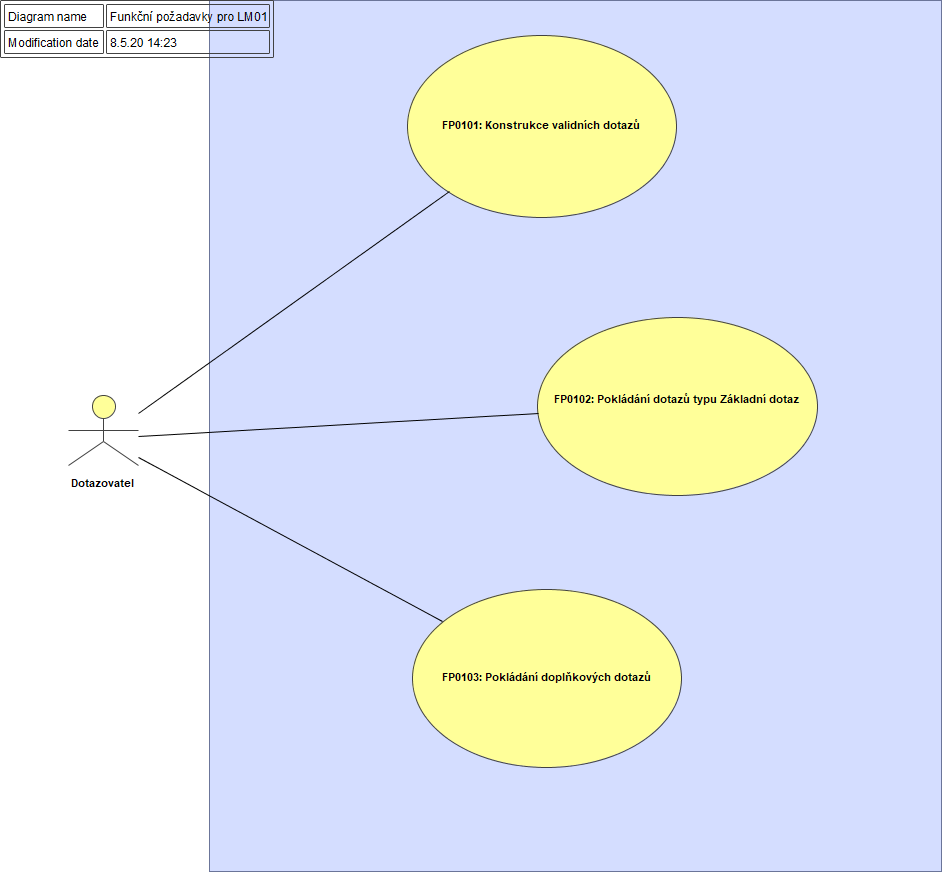
\includegraphics[width=\textwidth]{res/design/Funkční požadavky pro LM01.png}
  \caption{Logický modul LM01}
  \label{fig:Logický modul LM01}
\end{figure}

\begin{table}[H]
	\centering
	\begin{tabular}{|p{0.15\textwidth}|p{0.85\textwidth}|}
		\hline
  		{\textbf{ID}} & {\textbf{Požadavek}} \\
  		\hline \hline
  		FP0101 & \textbf{Konstrukce validních dotazů:} Q-systém umožní dotazovateli zkonstruovat validní dotazy z~hlediska nabízené funkcionality IS~AAAA, pomocí aktivní kontroly povolených kombinací typů dotazu, modifikátorů dotazu a typů entit, a zároveň vzhledem k~přiřazeným rolím neumožní tvorbu dotazu, na který dotazovatel nemá oprávnění.  \\ \hline
		FP0102 & \textbf{Pokládání dotazů typu \textit{Základní dotaz}:} Q-systém umožní dotazovateli explicitně položit textový dotaz typu \textit{Základní dotaz} do IS~AAAA a zobrazit odpověď na tento dotaz. \\ \hline
		FP0103 & \textbf{Pokládání doplňkových dotazů:} Q-systém umožní dotazovateli získat doplňující data k~odpovědi na dotaz typu \textit{Základní dotaz} pomocí doplňkových dotazů dvěma způsoby:
		\begin{enumerate}
			\item Vybráním automatického získání všech doplňujících dat u~konkrétního záznamu
			\item Ručním výběrem konkrétního doplňujícího údaje, který má být získán (například fotografie)
		\end{enumerate}
		\label{FP0103}
Doplňkové dotazy tedy nebude možné pokládat explicitně.  \\ \hline
	\end{tabular}
 	\caption{Funkční požadavky modulu LM01}
\label{tab:Funkční požadavky modulu LM01}
\end{table}

\subsubsection{LM02 Požadavky na správu konfigurace}
\label{LM02}
\begin{figure}[H]
  \centering
  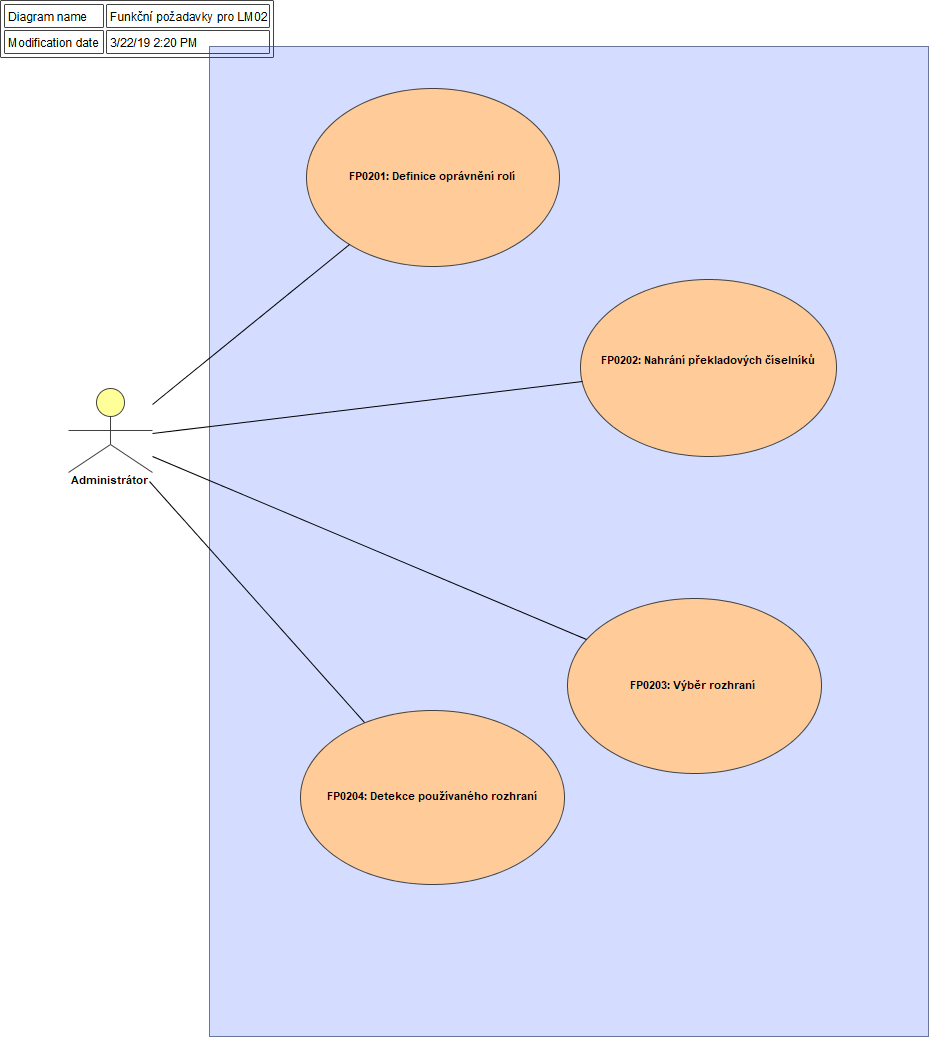
\includegraphics[width=\textwidth]{res/design/Funkční požadavky pro LM02.png}
  \caption{Logický modul LM02}
  \label{fig:Logický modul LM02}
\end{figure}

\begin{table}[H]
	\centering
	\begin{tabular}{|p{0.15\textwidth}|p{0.85\textwidth}|}
		\hline
  		{\textbf{ID}} & {\textbf{Požadavek}} \\
  		\hline \hline
  		FP0201 & \textbf{Definice oprávnění rolí:} Q-systém umožní administrátorovi definovat, jaké role mají povoleno pokládat dotazy určitého typu, s~určitým modifikátorem dotazu a na určité typy entit. Seznam definovaných rolí poskytne Active Directory.  \\ \hline
		FP0202 & \textbf{Nahrání překladových číselníků:} Q-systém umožní administrátorovi nahrát překladové číselníky, které budou využity při tvorbě dotazů. \\ \hline
		FP0203 & \textbf{Výběr rozhraní:} Q-systém bude posílat dotazy buď na standardní rozhraní \textit{Plné rozhraní}, nebo na rozhraní \textit{Zjednodušené rozhraní}. Q-systém umožní administrátorovi zvolit konkrétní rozhraní, pokud bude mít Q-systém nárok na obě. \\ \hline
		FP0204 & \textbf{Detekce používaného rozhraní:} Q-systém umožní administrátorovi zjistit, na které rozhraní IS AAAA se dotazy aktuálně pokládají. \\ \hline
	\end{tabular}
 	\caption{Funkční požadavky modulu LM02}
\label{tab:Funkční požadavky modulu LM02}
\end{table}

\subsubsection{LM03 Požadavky na autentizaci, autorizaci a logování}
\label{LM03}
\begin{figure}[H]
  \centering
  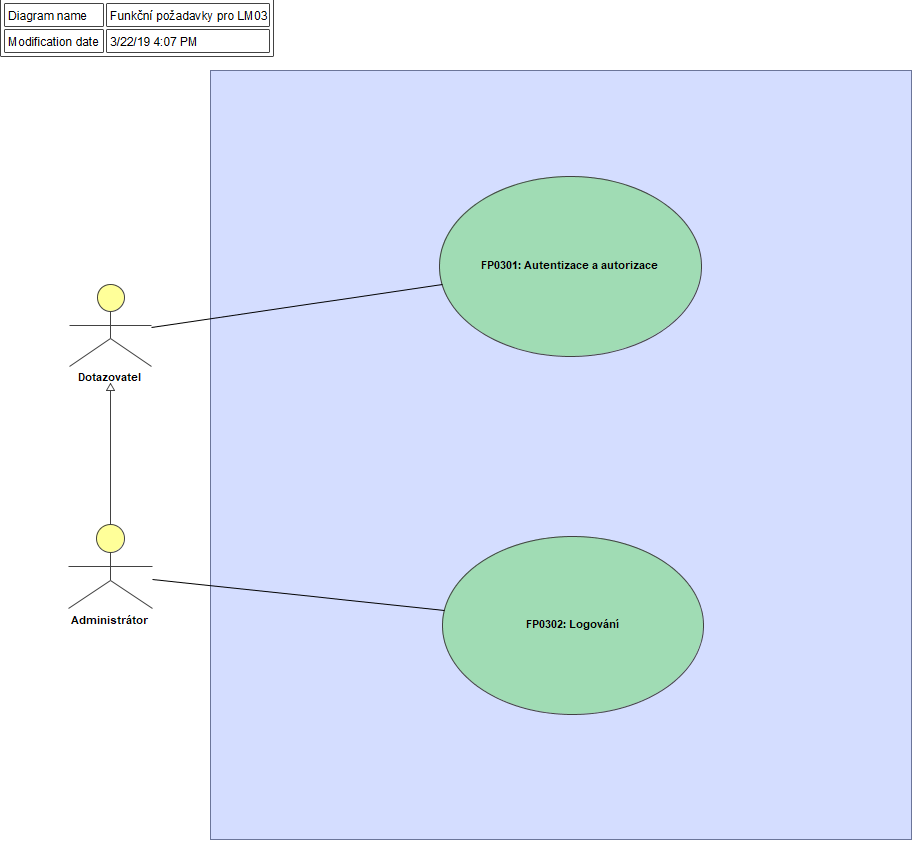
\includegraphics[width=\textwidth]{res/design/Funkční požadavky pro LM03.png}
  \caption{Logický modul LM03}
  \label{fig:Logický modul LM03}
\end{figure}

\begin{table}[H]
	\centering
	\begin{tabular}{|p{0.15\textwidth}|p{0.85\textwidth}|}
		\hline
  		{\textbf{ID}} & {\textbf{Požadavek}} \\
  		\hline \hline
  		FP0301 & \textbf{Autentizace a autorizace:} Q-systém umožní uživatelům se autentizovat oproti Active Directory z~prostředí zákazníka. Uživatelé Q-systému se budou autorizovat rolemi, které získají rovněž z~Active Directory.

Je zodpovědností zákazníka správně přiřadit svým uživatelům jednotlivé role. \\ \hline
		FP0302 & \textbf{Logování:} Q-systém bude logovat veškerou komunikaci s~IS~AAAA (položené dotazy, navrácené odpovědi). Logovat se bude také přihlášení vůči Active Directory. Dále se budou logovat veškeré akce modifikující konfiguraci Q-systému. Nad logy nebude prozatím žádná vyšší logika. Q-systém umožní administrátorovi přístup k~logům. \\ \hline
	\end{tabular}
 	\caption{Funkční požadavky modulu LM03}
\label{tab:Funkční požadavky modulu LM03}
\end{table}

\newpage
\subsection{Požadavky na výstupy}
Systém neposkytuje žádný očekávaný tiskový nebo exportní výstup.

\subsection{Nefunkční požadavky}
V~této kapitole jsou zahrnuty požadavky na obecné chování a vlastnosti systému.

\label{NefunkcniPozadavky}
\begin{table}[H]
	\centering
	\begin{tabular}{|p{0.15\textwidth}|p{0.85\textwidth}|}
		\hline
  		{\textbf{ID}} & {\textbf{Požadavek}} \\
  		\hline \hline
		PV01 & Systém bude založen na tzv. \textit{open-source} technologiích, aby cílový zákazník nebyl zatížen dodatečnými licenčními nároky. Cílová platforma je Linux (CentOS). \\ \hline
		PV02 & Systém bude určen pro jednotky, maximálně desítky uživatelů. Výkon Q-systému bude možné škálovat použitým HW. \\ \hline
		PV03 & Q-systém bude implementován jako tenký klient, komunikující se serverovou částí. \\ \hline
		PV04 & Q-systém bude distribuován jako samostatně fungující webová aplikace. \\ \hline
		PV05 & Q-systém bude replikovatelný a rozšiřitelný zákazníkem. \\ \hline
		PV06 & Napojení Q-systému na ostatní komponenty z~prostředí zákazníka nebude zodpovědností Q-systému. \\ \hline
		PV07 & Omezování rychlosti pokládání dotazů nebude implementováno v~rámci Q-systému. \\ \hline
		PV08 & Uživatelské rozhraní se přizpůsobí aktuálně používanému datovému rozhraní. Například pro rozhraní \textit{Zjednodušené rozhraní} nebude nabízena funkcionalita z~\hyperref[FP0103]{FP0103}, protože toto rozhraní umožňuje pouze pokládání dotazů typu \textit{Základní dotaz}. \\ \hline
		PV09 & Q-systém bude v~českém jazyce. \\ \hline
	\end{tabular}
 	\caption{Požadované vlastnosti systému}
\label{tab:Požadované vlastnosti systému}
\end{table}

\chapter{Návrh}
\label{Navrh}

\section{Doména}
V~této kapitole se nachází doménový diagram, který obsahuje nejdůležitější entity a vazby mezi nimi. Znalost domény usnadní pochopení následujících popisů scénářů případů užití.

\begin{figure}[H]
  \centering
  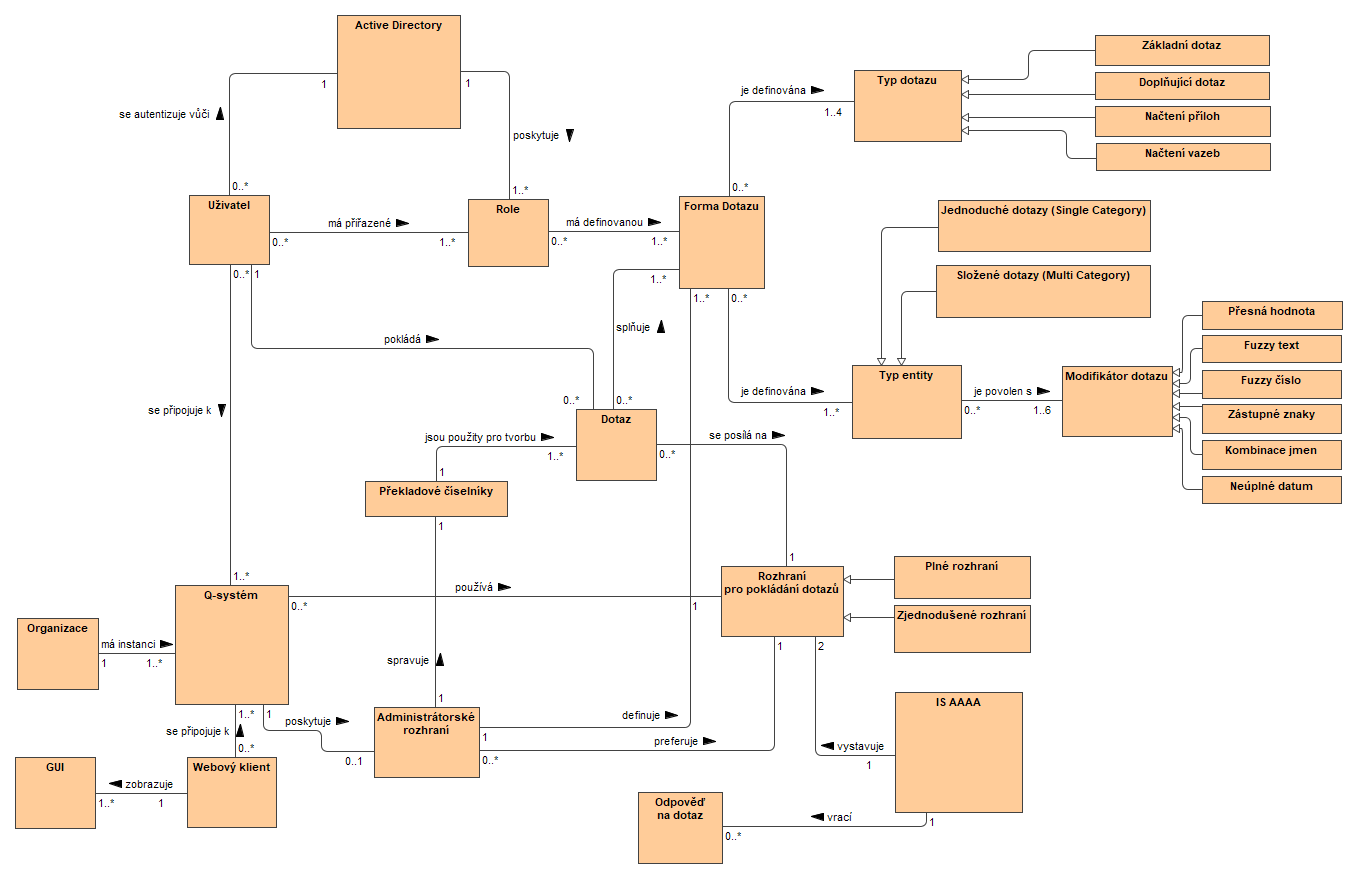
\includegraphics[width=\textwidth]{res/design/Doménový diagram.png}
  \caption{Doménový diagram}
  \label{fig:Doménový diagram}
\end{figure}

\section{Funkční specifikace}
Funkcionalita navrhované aplikace je popsána formou případů použití. Pro každý případ použití je vyplněna následující sada katalogových listů. Případy použití jsou z~důvodu přehlednosti a srozumitelnosti členěny do funkčních celků souhrnně popsaných níže.

Funkční celek sdružuje funkční požadavky spolu související, podobného charakteru často podporující stejný proces nebo podproces. Použité funkční celky nejsou přímým obrazem logických modulů použitých v~analytické části.

\begin{table}[H]
	\centering
	\begin{tabular}{|p{0.15\textwidth}|p{0.85\textwidth}|}
		\hline
  		{\textbf{ID}} & {\textbf{Název}} \\
  		\hline \hline
  		FC01 & \hyperref[FC01]{Pokládání dotazů} \\ \hline
		FC02 & \hyperref[FC02]{Správa konfigurace} \\ \hline
		FC03 & \hyperref[FC03]{Zobrazení logovaných informací} \\ \hline
		FC04 & \hyperref[FC04]{Autentizace a autorizace} \\ \hline
	\end{tabular}
 	\caption{Seznam funkčních celků}
\label{tab:Seznam funkčních celků}
\end{table}

\newpage
\subsection{FC01 Pokládání dotazů}
\label{FC01}
\begin{figure}[H]
  \centering
  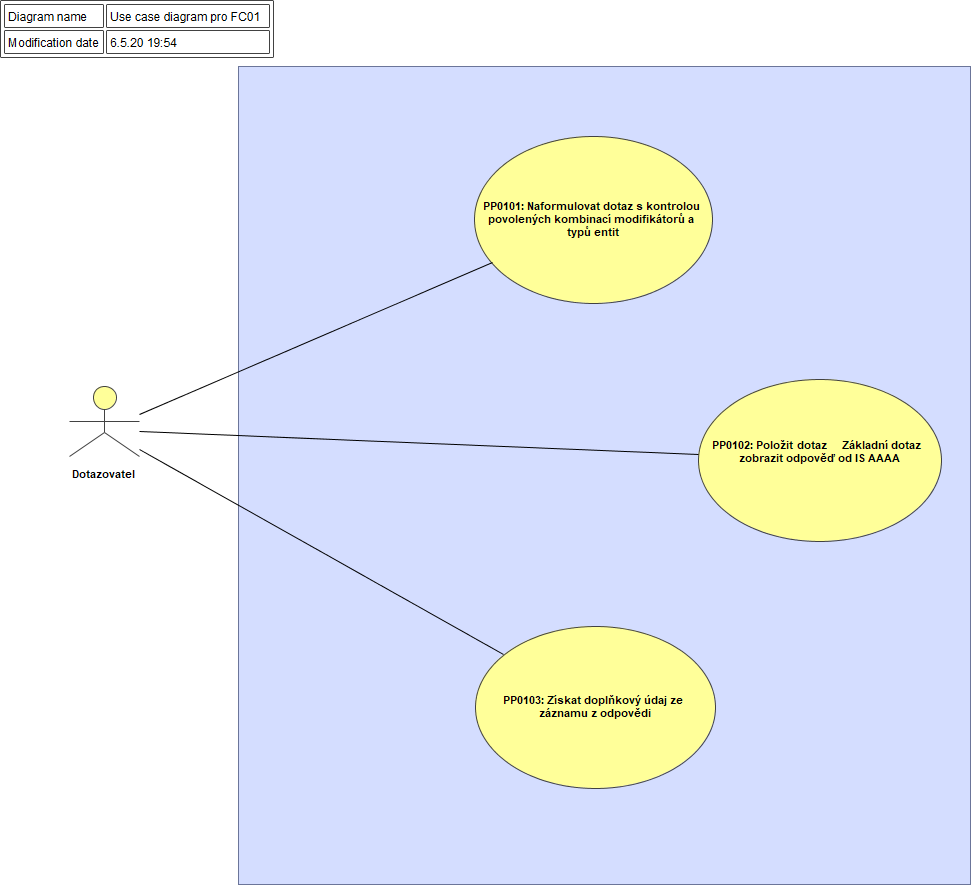
\includegraphics[width=\textwidth]{res/design/Use case diagram pro FC01.png}
  \caption{Funkční celek FC01 a jeho případy použití}
  \label{fig:Funkční celek FC01 a jeho případy použití}
\end{figure}

\newpage
\subsubsection{Případ použití PP0101}
	\begin{longtable}{|g|p{0.80\textwidth}|}
		\hline
		\rowcolor{Blue}\multicolumn{2}{|p{\textwidth}|}{\textbf{Naformulovat dotaz s~kontrolou povolených kombinací modifikátorů a typů entit}} \\ \hline
		\textbf{ID případu použití:} & PP0101 \\ \hline
		\textbf{ID požadavku:} & FP0101 \\ \hline
		\textbf{Cíl:} & Sestavit validní dotaz z~hlediska IS~AAAA, který zároveň respektuje také dotazovatelovy povolené formy dotazu. \\ \hline
		\textbf{Výchozí podmínky:} & Dotazovatel je přihlášen do systému. \\ \hline
		\textbf{Uživatel \slash Organizační role:} & Dotazovatel \\ \hline
		\textbf{Využití služeb jiných systémů:} & \\ \hline
		\textbf{Stav \mbox{po dokončení:}} & Na pozadí je vytvořen validní dotaz typu \textit{Základní dotaz} připravený k~\hyperref[ZaslaniDoISAAA]{zaslání do IS~AAAA}. \\ \hline
		\rowcolor{Gray}\multicolumn{2}{|l|}{\textbf{Popis, komentáře}} \\ \hline
		\multicolumn{2}{|p{\textwidth}|}{Tento případ popisuje, jakým způsobem dotazovatel naformuluje dotaz do IS~AAAA prostřednictvím GUI.} \\ \hline
		\caption{Případ použití PP0101}
		\label{tab:Případ použití PP0101}
	\end{longtable}
	\begin{longtable}{|p{0.07\textwidth}|p{0.93\textwidth}|}
		\rowcolor{Gray}\multicolumn{2}{|l|}{\textbf{Základní scénář}} \\ \hline
		\textbf{Krok} & \\ \hline
		1 & Dotazovatel vybere v~\hyperref[RozbalovaciMenu]{rozbalovacím menu} typ entity, na který se chce dotazovat, například \uv{Osoba}. \\ \hline
		2 & Systém zobrazí \hyperref[O02Dotaz]{formulář} pro vybraný typ entity, na kterém je možné zadat konkrétní vyhledávací kritéria (formou výběru z~výčtu, využívají \hyperref[PrekladoveCiselniky]{překladové číselníky}) a ke každému kritériu zvolit modifikátor (pokud je tak povoleno z~hlediska IS~AAAA, viz dokument Queries Description \cite{Queries}).  \\ \hline
		3 & Systém na základě povolených forem dotazu zneplatní modifikátory, které nelze použít s~vybraným typem entity. \\ \hline
		4 & Dotazovatel vyplní vyhledávací kritéria. \\ \hline
		5 & Dotazovatel může ke každému kritériu vybrat modifikátory. Pokud tak neučiní, je použit výchozí modifikátor \textit{Přesná hodnota}. \\ \hline
		6 & Systém na pozadí sestavuje validní dotaz typu \textit{Základní dotaz} připravený k~\hyperref[ZaslaniDoISAAA]{zaslání do IS~AAAA}. \\ \hline
		\caption{Scénář PP0101}
		\label{tab:Scénář PP0101}
	\end{longtable}

\newpage
\subsubsection{Případ použití PP0102}
	\begin{longtable}{|g|p{0.80\textwidth}|}
		\hline
		\rowcolor{Blue}\multicolumn{2}{|l|}{\textbf{Položit dotaz typu \textit{Základní dotaz} a zobrazit odpověď od IS~AAAA}} \\ \hline
		\textbf{ID případu použití:} & PP0102 \\ \hline
		\textbf{ID požadavku:} & FP0102 \\ \hline
		\textbf{Cíl:} & Položit uživatelem naformulovaný dotaz a zobrazit odpověď na tento dotaz. \\ \hline
		\textbf{Výchozí podmínky:} & Dotazovatel naformuloval dotaz. \\ \hline
		\textbf{Uživatel \slash Organizační role:} & Dotazovatel \\ \hline
		\textbf{Využití služeb jiných systémů:} & Rozhraní s~IS~AAAA \\ \hline
		\textbf{Stav \mbox{po dokončení:}} & Uživatel má zobrazenou odpověď, ve které jsou patrné doplňkové údaje, které lze dále získat. \\ \hline
		\rowcolor{Gray}\multicolumn{2}{|l|}{\textbf{Popis, komentáře}} \\ \hline
		\multicolumn{2}{|p{\textwidth}|}{Tento případ popisuje, co bude zobrazeno uživateli a jaké doplňující údaje mu budou dále umožněny získat.} \\ \hline
		\caption{Případ použití PP0102}
		\label{Případ použití PP0102}
	\end{longtable}
	\begin{longtable}{|p{0.07\textwidth}|p{0.93\textwidth}|}
		\rowcolor{Gray}\multicolumn{2}{|l|}{\textbf{Základní scénář}} \\ \hline
		\textbf{Krok} & \\ \hline
		\label{ZaslaniDoISAAA}
		1 & Dotazovatel zvolí možnost \uv{Odeslat dotaz} na \hyperref[O02Dotaz]{formuláři s~vyplněnými vyhledávacími kritérii}. \\ \hline
		2 & Systém si ze své \hyperref[Konfigurace]{konfigurace} zjistí, jaké rozhraní IS~AAAA pro pokládání dotazů se aktuálně používá. \\ \hline
		3 & Systém naformulovaný dotaz zabalí do finálního dotazu, který ve hlavičce má \textit{namespace} odpovídající aktuálně používanému rozhraní IS~AAAA. \\ \hline
		4 & Systém odešle vytvořený dotaz synchronní komunikací na aktuálně používané rozhraní IS~AAAA a vyčká na odpověď. \\ \hline
		5 & Systém zaloguje položený dotaz i odpověď do \hyperref[Logy]{audit logu komunikace s~IS~AAAA}. \\ \hline
		6 & Systém provede XSLT transformaci odpovědi od IS~AAAA na strukturu dat, která mají být zobrazena v~GUI. \\ \hline
		7 & Systém \hyperref[O03OdpovedNaDotaz]{zobrazí odpověď} ve formě seznamu nalezených kandidátů. Systém umožní zobrazit \hyperref[O04DetailKandidata]{detail konkrétního kandidáta}. \\ \hline
		8 & Pokud má dotazovatel oprávnění pokládat dotazy typu \textit{Doplňující dotaz}, systém přidá ikonu ke všem vazbám v~seznamu kandidátů, která symbolizuje možnost získat doplňující údaje o~připojeném záznamu.

Pokud má dotazovatel oprávnění pokládat dotazy typu \textit{Načtení příloh}, systém přidá možnost stažení ke všem přílohám v~seznamu. Systém dále přidá možnost zobrazení doplňkového údaje k~takovým binárním datům, které mají v~metadatech definováno, že se jedná o~obrázky (typ souboru je JPEG, GIF, TIFF, PNG, BMP nebo PDF).

Pokud má dotazovatel oprávnění pokládat dotazy typu \textit{Načtení vazeb}, systém přidá možnost stažení a ikonu umožňující zobrazení této vazby.  \\ \hline
		\rowcolor{Gray}\multicolumn{2}{|l|}{\textbf{Alternativní scénáře}} \\ \hline
		\textbf{Krok} & \\ \hline
		6a &
		6a1 Z~odpovědi od IS~AAAA je patrné, že certifikát, jakým se systém prokazuje, nemá dostatečné oprávnění na rozhraní, na které byl dotaz poslán.

  		6a2 Pokud je aktuálně používané rozhraní \textit{Plné rozhraní}, systém automaticky ve své \hyperref[Konfigurace]{konfiguraci} změní aktuálně používané rozhraní na \textit{Zjednodušené rozhraní}.

  		6a3 Systém zaloguje změnu aktuálně používaného rozhraní do \hyperref[Logy]{logu provedených akcí v~administrátorském rozhraní}.

  		6a4 Systém se pokusí opakovaně odeslat dotaz, tzn. scénář pokračuje krokem 3.
 \\ \hline
		6b & Odpověď od IS~AAAA obsahuje informaci o~chybě, systém informuje uživatele. \\ \hline
		\caption{Scénář PP0102}
		\label{tab:Scénář PP0102}
	\end{longtable}

\newpage
\subsubsection{Případ použití PP0103}
	\begin{longtable}{|g|p{0.80\textwidth}|}
		\hline
		\rowcolor{Blue}\multicolumn{2}{|l|}{\textbf{Získat doplňkový údaj ze záznamu z~odpovědi}} \\ \hline
		\textbf{ID případu použití:} & PP0103 \\ \hline
		\textbf{ID požadavku:} & FP0103 \\ \hline
		\textbf{Cíl:} & Zobrazit nebo stáhnout doplňkový údaj z~konkrétního záznamu. \\ \hline
		\textbf{Výchozí podmínky:} & Dotazovatel položil dotaz a v~odpovědi přišel alespoň 1 záznam, který obsahuje vazbu na připojený záznam. Zároveň dotazovatel má přiřazenou roli, která mu povoluje pokládat typy dotazů, které umožňují získávat doplňkové údaje (\textit{Doplňující dotaz}, \textit{Načtení příloh}, \textit{Načtení vazeb}). \\ \hline
		\textbf{Uživatel \slash Organizační role:} & Dotazovatel \\ \hline
		\textbf{Využití služeb jiných systémů:} & \\ \hline
		\textbf{Stav \mbox{po dokončení:}} & Dotazovatel má zobrazen\slash stažen daný doplňkový údaj. \\ \hline
		\rowcolor{Gray}\multicolumn{2}{|l|}{\textbf{Popis, komentáře}} \\ \hline
		\multicolumn{2}{|p{\textwidth}|}{Tento případ popisuje způsob pokládání doplňkových dotazů a zobrazení odpovědí na základě typu doplňkového údaje.} \\ \hline
		\caption{Případ použití PP0103}
		\label{tab:Případ použití PP0103}
	\end{longtable}
\newpage
	\begin{longtable}{|p{0.07\textwidth}|p{0.93\textwidth}|}
		\rowcolor{Gray}\multicolumn{2}{|l|}{\textbf{Základní scénář}} \\ \hline
		\textbf{Krok} & \\ \hline
		1 & Dotazovatel klikne na \hyperref[O04DetailKandidata]{ikonu lupy} umožňující zobrazení doplňkového údaje (text, vazba, příloha). \\ \hline
		2 & Systém na pozadí vytvoří validní doplňkový dotaz připravený k~zaslání do IS~AAAA.

Pokud dotazovatel chce získat doplňující informace ke konkrétnímu záznamu, systém vytvoří dotaz typu \textit{Doplňující dotaz}, dotazující se na \texttt{AAA\_ID} konkrétního záznamu.

Pokud dotazovatel chce získat přílohy ke konkrétnímu záznamu, systém vytvoří dotaz typu \textit{Načtení příloh}, dotazující se na \texttt{AAA\_ID} konkrétního záznamu a \texttt{ID\_Prilohy}.

Pokud dotazovatel chce získat připojenou vazbu u~konkrétního záznamu, systém vytvoří dotaz typu \textit{Načtení vazeb} dotazující se na \texttt{AAA\_ID} konkrétního záznamu a \texttt{ID\_Vazby}.
 \\ \hline
		3 & Systém si ze své \hyperref[Konfigurace]{konfigurace} zjistí, jaké rozhraní IS~AAAA pro pokládání dotazů se aktuálně používá. \\ \hline
		4 & Systém odešle vytvořený dotaz synchronní komunikací na aktuálně používané rozhraní IS~AAAA a vyčká na odpověď. \\ \hline
		5 & Systém zaloguje položený dotaz i odpověď do \hyperref[Logy]{audit logu komunikace s~IS~AAAA}. \\ \hline
		6 & Systém zobrazí odpověď na doplňkový dotaz v~nové záložce prohlížeče.

Pokud se jednalo o~dotaz typu \textit{Doplňující dotaz}, odpověď je transformována na odpověď od dotazu typu \textit{Základní dotaz}. Viz \hyperref[cqrd]{Transformace odpovědi na dotaz typu \textit{Doplňující dotaz}}.
Dále se aplikuje stejná XLST transformace, jako v~\hyperref[ZaslaniDoISAAA]{PP102 krok 6}.

Pokud se jednalo o~dotaz typu \textit{Načtení příloh}, systém zobrazí binární data ve formě fotografie.

Pokud se jednalo o~dotaz typu \textit{Načtení vazeb}, systém zobrazí graf vazeb jako naskenovaný dokument.
 \\ \hline
		\rowcolor{Gray}\multicolumn{2}{|l|}{\textbf{Alternativní scénáře}} \\ \hline
		\textbf{Krok} & \\ \hline
		1a &
		1a1 Dotazovatel vybere automatické získání všech doplňujících údajů pro konkrétní záznam z~odpovědi.

		1a2 Systém získá každý doplňující údaj a zobrazí ho v~nové záložce prohlížeče dle základního scénáře tohoto případu užití.
\\ \hline
		\caption{Scénář PP0103}
		\label{tab:Scénář PP0103}
	\end{longtable}


\subsection{FC02 Správa konfigurace}
\label{FC02}
\begin{figure}[H]
  \centering
  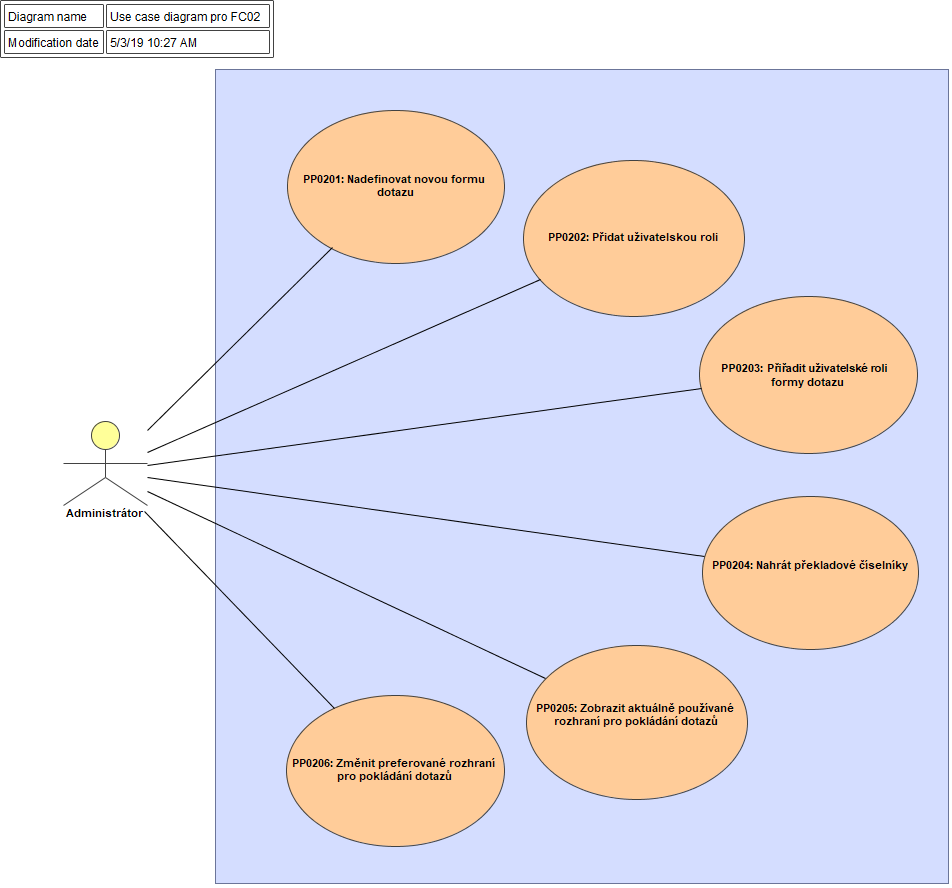
\includegraphics[width=\textwidth]{res/design/Use case diagram pro FC02.png}
  \caption{Funkční celek FC02 a jeho případy použití}
  \label{fig:Funkční celek FC02 a jeho případy použití}
\end{figure}

\newpage
\subsubsection{Případ použití PP0201}
	\begin{longtable}{|g|p{0.80\textwidth}|}
		\hline
		\rowcolor{Blue}\multicolumn{2}{|l|}{\textbf{Nadefinovat novou formu dotazu}} \\ \hline
		\textbf{ID případu použití:} & PP0201 \\ \hline
		\textbf{ID požadavku:} & FP0201 \\ \hline
		\textbf{Cíl:} & Nadefinovat novou formu dotazu, kterou bude možné přiřadit uživatelským rolím. \\ \hline
		\textbf{Výchozí podmínky:} & Administrátor je přihlášen do systému. \\ \hline
		\textbf{Uživatel \slash Organizační role:} & Administrátor \\ \hline
		\textbf{Využití služeb jiných systémů:} & \\ \hline
		\textbf{Stav \mbox{po dokončení:}} & V~\hyperref[Konfigurace]{konfiguraci} přibyla nová forma dotazu. \\ \hline
		\rowcolor{Gray}\multicolumn{2}{|l|}{\textbf{Popis, komentáře}} \\ \hline
		\multicolumn{2}{|p{\textwidth}|}{Tento případ popisuje způsob definice nové formy dotazu.} \\ \hline
		\caption{Případ použití PP0201}
		\label{tab:Případ použití PP0201}
	\end{longtable}
\newpage
	\begin{longtable}{|p{0.07\textwidth}|p{0.93\textwidth}|}
		\rowcolor{Gray}\multicolumn{2}{|l|}{\textbf{Základní scénář}} \\ \hline
		\textbf{Krok} & \\ \hline
		1 & Administrátor vybere v~\hyperref[RozbalovaciMenu]{rozbalovacím menu} volbu \uv{Formy dotazu}. \\ \hline
		2 & Vstup do administrace forem dotazu systém zaloguje do \hyperref[Logy]{logu provedených akcí v~administrátorském rozhraní}. \\ \hline
		3 & Systém zobrazí \hyperref[O05FormyDotazu]{formulář}, na kterém je seznam definovaných forem dotazu (získaný z~\hyperref[Konfigurace]{konfigurace}), a který umožňuje vytvořit novou formu dotazu.  \\ \hline
		4 & Administrátor vyplní jméno nové formy dotazu, stručný popis a zvolí možnost \uv{Vytvořit}. \\ \hline
		5 & Systém zkontroluje, zda je zadané jméno unikátní. \\ \hline
		6 & Systém přidá novou formu dotazu do seznamu definovaných forem dotazu. Nová forma dotazu zatím nic nepovoluje. \\ \hline
		7 & Administrátor vstoupí do \hyperref[O06FormaDotazuDetail]{detailu nové formy dotazu}. \\ \hline
		8 & Administrátor v~sekci \uv{Typy dotazu} vybere 1 -- 4 typy dotazu, které bude tato forma povolovat. Výběr bude formou zaškrtávání \textit{checkboxů}. \\ \hline
		9 & Administrátor ke každému zvolenému typu entit může vybrat 1 -- 5 modifikátorů, které bude tato forma v~kombinaci s~konkrétním typem entity povolovat. Výběr bude formou zaškrtávání \textit{checkboxů}. Defaultně je povolen modifikátor \textit{Přesná hodnota}. \\ \hline
		10 & Administrátor potvrdí vytvoření nové formy dotazu volbou \uv{Uložit}. \\ \hline
		11 & Systém vytvoří formu dotazu a přidá ji do své \hyperref[Konfigurace]{konfigurace} do seznamu všech definovaných forem dotazu. \\ \hline
		12 & Systém zaloguje vytvoření nové formy dotazu do \hyperref[Logy]{logu provedených akcí v~administrátorském rozhraní}. \\ \hline
		\rowcolor{Gray}\multicolumn{2}{|l|}{\textbf{Alternativní scénáře}} \\ \hline
		\textbf{Krok} & \\ \hline
		5a &
		5a1 Pokud jméno nové formy dotazu není unikátní, systém vyzve administrátora k~opětovnému zadání unikátního jména.
		
   		5a2 Pokračuje se krokem 4 základního scénáře. \\ \hline
   		\caption{Scénář PP0201}
		\label{tab:Scénář PP0201}
	\end{longtable}

\newpage
\subsubsection{Případ použití PP0202}
	\begin{longtable}{|g|p{0.80\textwidth}|}
		\hline
		\rowcolor{Blue}\multicolumn{2}{|l|}{\textbf{Přidat uživatelskou roli}} \\ \hline
		\textbf{ID případu použití:} & PP0202 \\ \hline
		\textbf{ID požadavku:} & FP0201, FP0301 \\ \hline
		\textbf{Cíl:} & Přidat do systému uživatelskou roli, která již byla nebo bude přidána také do Active Directory. \\ \hline
		\textbf{Výchozí podmínky:} & Administrátor je přihlášen do systému. \\ \hline
		\textbf{Uživatel \slash Organizační role:} & Administrátor \\ \hline
		\textbf{Využití služeb jiných systémů:} & \\ \hline
		\textbf{Stav \mbox{po dokončení:}} & V~\hyperref[Konfigurace]{konfiguraci} přibyla nová uživatelská role. \\ \hline
		\rowcolor{Gray}\multicolumn{2}{|l|}{\textbf{Popis, komentáře}} \\ \hline
		\multicolumn{2}{|p{\textwidth}|}{Tento případ popisuje způsob zachování konzistence mezi definovanými uživateli v~Active Directory a mezi uživateli systému. Pokud dotazovatel má přiřazenou novou roli, může pokládat dotazy teprve poté, co je tato nová role zavedena jak Active Directory, tak v~systému. Zavedení nové role může být provedeno v~libovolném pořadí. Lze tedy nejprve přidat roli do systému a teprve následně do Active Directory, nebo naopak.} \\ \hline
		\caption{Případ použití PP0202}
		\label{tab:Případ použití PP0202}
	\end{longtable}
\newpage
	\label{PP0202}
	\begin{longtable}{|p{0.07\textwidth}|p{0.93\textwidth}|}
		\rowcolor{Gray}\multicolumn{2}{|l|}{\textbf{Základní scénář}} \\ \hline
		\textbf{Krok} & \\ \hline
		1 & Administrátor vybere v~\hyperref[RozbalovaciMenu]{rozbalovacím menu} volbu \uv{Uživatelské role}. \\ \hline
		2 & Vstup do administrace uživatelských rolí systém zaloguje do \hyperref[Logy]{logu provedených akcí v~administrátorském rozhraní}. \\ \hline
		3 & Systém zobrazí \hyperref[O07UzivatelskeRole]{formulář}, na kterém je seznam uživatelských rolí (získaný z~konfigurace), a který umožňuje přidat novou roli. \\ \hline
		4 & Administrátor vyplní jméno nové role, stručný popis a zvolí možnost \uv{Vytvořit}. \\ \hline
		5 & Systém zkontroluje, zda je zadané jméno unikátní. \\ \hline
		6 & Systém roli přidá do své \hyperref[Konfigurace]{konfigurace} do seznamu všech známých rolí. \\ \hline
		7 & Systém zaloguje přidání nové role do \hyperref[Logy]{logu provedených akcí v~administrátorském rozhraní}. \\ \hline
		\rowcolor{Gray}\multicolumn{2}{|l|}{\textbf{Alternativní scénáře}} \\ \hline
		\textbf{Krok} & \\ \hline
		5a &
   		5a1 Pokud jméno role není unikátní, systém vyzve administrátora k~opětovnému zadání unikátního jména.
   		
   		5a2 Pokračuje se krokem 4 základního scénáře.  \\ \hline
   		\caption{Scénář PP0202}
		\label{tab:Scénář PP0202}
	\end{longtable}

\newpage
\subsubsection{Případ použití PP0203}
	\begin{longtable}{|g|p{0.80\textwidth}|}
		\hline
		\rowcolor{Blue}\multicolumn{2}{|l|}{\textbf{Přiřadit uživatelské roli formy dotazu}} \\ \hline
		\textbf{ID případu použití:} & PP0203 \\ \hline
		\textbf{ID požadavku:} & FP0201 \\ \hline
		\textbf{Cíl:} & Přiřadit konkrétní uživatelské roli jednu nebo více forem dotazu. \\ \hline
		\textbf{Výchozí podmínky:} & Administrátor je přihlášen do systému. Je definována alespoň 1 forma dotazu a alespoň 1 uživatelská role. \\ \hline
		\textbf{Uživatel \slash Organizační role:} & Administrátor \\ \hline
		\textbf{Využití služeb jiných systémů:} & \\ \hline
		\textbf{Stav \mbox{po dokončení:}} & Uživatelská role nyní povoluje další nebo novou formu dotazu. \\ \hline
		\rowcolor{Gray}\multicolumn{2}{|l|}{\textbf{Popis, komentáře}} \\ \hline
		\multicolumn{2}{|p{\textwidth}|}{Tento případ popisuje postup, jak přiřadit konkrétní uživatelské roli jednu nebo více forem dotazu.} \\ \hline
		\caption{Případ použití PP0203}
		\label{tab:Případ použití PP0203}
	\end{longtable}
	\begin{longtable}{|p{0.07\textwidth}|p{0.93\textwidth}|}
		\rowcolor{Gray}\multicolumn{2}{|l|}{\textbf{Základní scénář}} \\ \hline
		\textbf{Krok} & \\ \hline
		1 & Administrátor vybere v~\hyperref[RozbalovaciMenu]{rozbalovacím menu} volbu \uv{Uživatelské role}. \\ \hline
		2 & Vstup do administrace uživatelských rolí systém zaloguje \hyperref[Logy]{do logu provedených akcí v~administrátorském rozhraní}. \\ \hline
		3 & Systém zobrazí \hyperref[O07UzivatelskeRole]{formulář}, na kterém je seznam uživatelských rolí (získaný z~\hyperref[Konfigurace]{konfigurace}). \\ \hline
		4 & Administrátor vstoupí do \hyperref[O08UzivatelskaRoleDetail]{detailu uživatelské role}, ke které chce přiřadit formy dotazu. \\ \hline
		5 & Systém zobrazí seznam všech forem dotazu ve dvojici s~\textit{checkboxy}, které jsou zaškrtnuté, pokud role povoluje danou formu dotazu (seznam forem dotazu i mapování rolí na formy dotazu, oboje získané z~\hyperref[Konfigurace]{konfigurace}). \\ \hline
		6 & Administrátor zaškrtne jednu nebo více forem dotazu a zvolí volbu \uv{Uložit}. \\ \hline
		7 & Systém v~\hyperref[Konfigurace]{konfiguraci} přiřadí k~roli vybrané formy dotazu. \\ \hline
		8 & Systém zaloguje přiřazení nových forem dotazu k~uživatelské roli do \hyperref[Logy]{logu provedených akcí v~administrátorském rozhraní}. \\ \hline
		\caption{Scénář PP0203}
		\label{tab:Scénář PP0203}
	\end{longtable}

\newpage
\subsubsection{Případ použití PP0204}
	\begin{longtable}{|g|p{0.80\textwidth}|}
		\hline
		\rowcolor{Blue}\multicolumn{2}{|l|}{\textbf{Nahrát překladové číselníky}} \\ \hline
		\textbf{ID případu použití:} & PP0204 \\ \hline
		\textbf{ID požadavku:} & FP0202 \\ \hline
		\textbf{Cíl:} & Přepsat stávající překladové číselníky novými. \\ \hline
		\textbf{Výchozí podmínky:} & Administrátor je přihlášen do systému. \\ \hline
		\textbf{Uživatel \slash Organizační role:} & Administrátor \\ \hline
		\textbf{Využití služeb jiných systémů:} & \\ \hline
		\textbf{Stav \mbox{po dokončení:}} & V~\hyperref[Konfigurace]{konfiguraci} jsou uloženy nové překladové číselníky, které jsou připraveny pro tvorbu následujících dotazů. \\ \hline
		\rowcolor{Gray}\multicolumn{2}{|l|}{\textbf{Popis, komentáře}} \\ \hline
		\multicolumn{2}{|p{\textwidth}|}{Tento případ popisuje způsob nahrání nových překladových číselníků do systému.} \\ \hline
		\caption{Případ použití PP0204}
		\label{tab:Případ použití PP0204}
	\end{longtable}
	\begin{longtable}{|p{0.07\textwidth}|p{0.93\textwidth}|}
		\rowcolor{Gray}\multicolumn{2}{|l|}{\textbf{Základní scénář}} \\ \hline
		\label{PP0204}
		\textbf{Krok} & \\ \hline
		1 & Administrátor vybere v~\hyperref[RozbalovaciMenu]{rozbalovacím menu} volbu \uv{Překladové číselníky}. \\ \hline
		2 & Vstup do administrace překladových číselníků systém zaloguje do \hyperref[Logy]{logu provedených akcí v~administrátorském rozhraní}. \\ \hline
		3 & Systém zobrazí \hyperref[O09PrekladoveCiselniky]{formulář} umožňující nahrát překladové číselníky. \\ \hline
		4 & Administrátor zvolí volbu \uv{Aktualizovat}. \\ \hline
		5 & Systém otevře souborový prohlížeč. \\ \hline
		6 & Administrátor vybere konfigurační \hyperref[PrekladoveCiselniky]{soubor s~novými číselníky}. \\ \hline
		7 & Systém ve své \hyperref[Konfigurace]{konfiguraci} nahradí původní překladové číselníky za nové. \\ \hline
		8 & Systém zaloguje nahrání nových překladových číselníků do \hyperref[Logy]{logu provedených akcí v~administrátorském rozhraní}. \\ \hline
		\caption{Scénář PP0204}
		\label{tab:Scénář PP0204}
	\end{longtable}

\newpage
\subsubsection{Případ použití PP0205}
	\begin{longtable}{|g|p{0.80\textwidth}|}
		\hline
		\rowcolor{Blue}\multicolumn{2}{|l|}{\textbf{Zobrazit aktuálně používané rozhraní pro pokládání dotazů}} \\ \hline
		\textbf{ID případu použití:} & PP0205 \\ \hline
		\textbf{ID požadavku:} & FP0204  \\ \hline
		\textbf{Cíl:} & Zjistit rozhraní IS~AAAA, které se aktuálně používá při pokládání dotazů. \\ \hline
		\textbf{Výchozí podmínky:} & Administrátor je přihlášen do systému. \\ \hline
		\textbf{Uživatel \slash Organizační role:} & Administrátor, Dotazovatel \\ \hline
		\textbf{Stav \mbox{po dokončení:}} & Je znám název aktuálně používaného rozhraní. \\ \hline
		\rowcolor{Gray}\multicolumn{2}{|l|}{\textbf{Popis, komentáře}} \\ \hline
		\multicolumn{2}{|p{\textwidth}|}{Tento případ popisuje, jak může administrátor zjistit, na které rozhraní IS~AAAA systém na pozadí pokládá dotazy.

Poznámka: Tuto skutečnost může poznat i dotazovatel bez administrátorského rozhraní. Je tomu tak, protože rozhraní \textit{Zjednodušené rozhraní}, nezpracovává jiné dotazy než dotazy typu \textit{Základní dotaz}. Pokud dotazovatel bude vědět, že má přiřazenou roli, která mu povoluje pokládat doplňkové dotazy, ale systém mu je neumožní položit, bude mu jasné, že systém aktuálně musí používat rozhraní \textit{Zjednodušené rozhraní}.
} \\ \hline
		\caption{Případ použití PP0205}
		\label{tab:Případ použití PP0205}
	\end{longtable}
	\begin{longtable}{|p{0.07\textwidth}|p{0.93\textwidth}|}
		\rowcolor{Gray}\multicolumn{2}{|l|}{\textbf{Základní scénář}} \\ \hline
		\textbf{Krok} & \\ \hline
		1 & Administrátor vybere v~\hyperref[RozbalovaciMenu]{rozbalovacím menu} volbu \uv{Rozhraní na IS~AAAA}. \\ \hline
		2 & Vstup do administrace rozhraní na IS~AAAA systém zaloguje do \hyperref[Logy]{logu provedených akcí v~administrátorském rozhraní}. \\ \hline
		3 & Systém v~sekci \uv{Aktuálně používané rozhraní} zobrazí název aktuálně používaného rozhraní (dle \hyperref[Konfigurace]{konfigurace}) na příslušném \hyperref[O10RozhraniNaISAAA]{formuláři}. \\ \hline
		\rowcolor{Gray}\multicolumn{2}{|l|}{\textbf{Alternativní scénáře}} \\ \hline
		\textbf{Krok} & \\ \hline
		1a & Administrátor i Dotazovatel mohou vidět aktuálně používané rozhraní v~\hyperref[HorniLista]{horní liště aplikace}. \\ \hline
		\caption{Scénář PP0205}
		\label{tab:Scénář PP0205}
	\end{longtable}

\newpage
\subsubsection{Případ použití PP0206}
	\begin{longtable}{|g|p{0.80\textwidth}|}
		\hline
		\rowcolor{Blue}\multicolumn{2}{|l|}{\textbf{Změnit preferované rozhraní pro pokládání dotazů}} \\ \hline
		\textbf{ID případu použití:} & PP0206 \\ \hline
		\textbf{ID požadavku:} & FP0203  \\ \hline
		\textbf{Cíl:} & Vybrat rozhraní, které se má preferovat jako aktuálně používané rozhraní pro pokládání dotazů. \\ \hline
		\textbf{Výchozí podmínky:} & Administrátor je přihlášen do systému. \\ \hline
		\textbf{Uživatel \slash Organizační role:} & Administrátor \\ \hline
		\textbf{Využití služeb jiných systémů:} & \\ \hline
		\textbf{Stav \mbox{po dokončení:}} & V~\hyperref[Konfigurace]{konfiguraci} je jako preferované rozhraní definováno vybrané rozhraní a zároveň se v~\hyperref[Konfigurace]{konfiguraci} změnilo aktuálně používané rozhraní na vybrané rozhraní. \\ \hline
		\rowcolor{Gray}\multicolumn{2}{|l|}{\textbf{Popis, komentáře}} \\ \hline
		\multicolumn{2}{|p{\textwidth}|}{Tento případ popisuje výběr preferovaného rozhraní pro pokládání následujících dotazů. Je potřeba brát v~potaz, že pokud bude dotaz položen na rozhraní, na který z~hlediska certifikátu nemá oprávnění, potom se dotazovateli zobrazí informace o~chybě. Nemá smysl preferovat rozhraní \textit{Plné rozhraní}, pokud je dle certifikátu nárok pouze na \textit{Zjednodušené rozhraní}. Naopak ovšem dává smysl, že systém sice má nárok na rozhraní \textit{Plné rozhraní}, ovšem administrátor toto rozhraní nechce zatěžovat a vybere rozhraní \textit{Zjednodušené rozhraní} jako preferované pro pokládání dotazů.} \\ \hline
		\caption{Případ použití PP0206}
		\label{tab:Případ použití PP0206}
	\end{longtable}
\newpage
	\begin{longtable}{|p{0.07\textwidth}|p{0.93\textwidth}|}
		\rowcolor{Gray}\multicolumn{2}{|l|}{\textbf{Základní scénář}} \\ \hline
		\textbf{Krok} & \\ \hline
		1 & Administrátor vybere v~\hyperref[RozbalovaciMenu]{rozbalovacím menu} volbu \uv{Rozhraní na IS~AAAA}. \\ \hline
		2 & Vstup do administrace rozhraní na IS~AAAA systém zaloguje \hyperref[Logy]{do logu provedených akcí v~administrátorském rozhraní}. \\ \hline
		3 & Administrátor v~sekci \uv{Preferované rozhraní} vybere možnost \uv{Změnit}.  \\ \hline
		4 & Systém zobrazí \hyperref[O11ZmenaRozhraniNaISAAA]{formulář} umožňující výběr mezi rozhraními IS~AAAA. \\ \hline
		5 & Administrátor vybere preferované rozhraní, na které chce, aby dotazovatelé pokládali dotazy a potvrdí kliknutím na \uv{Uložit}. Výběr bude formou \textit{radiobuttonů}. \\ \hline
		6 & Systém ve své \hyperref[Konfigurace]{konfiguraci} přepíše preferované a také aktuálně používané rozhraní pro pokládání dotazů. \\ \hline
		7 & Systém zaloguje změnu preferovaného rozhraní a aktuálně používaného rozhraní do \hyperref[Logy]{logu provedených akcí v~administrátorském rozhraní}. \\ \hline
		\rowcolor{Gray}\multicolumn{2}{|l|}{\textbf{Alternativní scénáře}} \\ \hline
		\textbf{Krok} & \\ \hline
		3a &
		3a1 Administrátor v~sekci \uv{Aktuálně používané rozhraní} vybere možnost \uv{Nastavit na preferované}.
		
  		3a2 Systém ve své \hyperref[Konfigurace]{konfiguraci} přepíše preferované rozhraní na aktuálně používané rozhraní.
  		
  		3a3 Systém zaloguje změnu preferovaného rozhraní do \hyperref[Logy]{logu provedených akcí v~administrátorském rozhraní}. \\ \hline
  		\caption{Scénář PP0206}
		\label{tab:Scénář PP0206}
	\end{longtable}


\subsection{FC03 Zobrazení logovaných informací}
\label{FC03}
\begin{figure}[H]
  \centering
  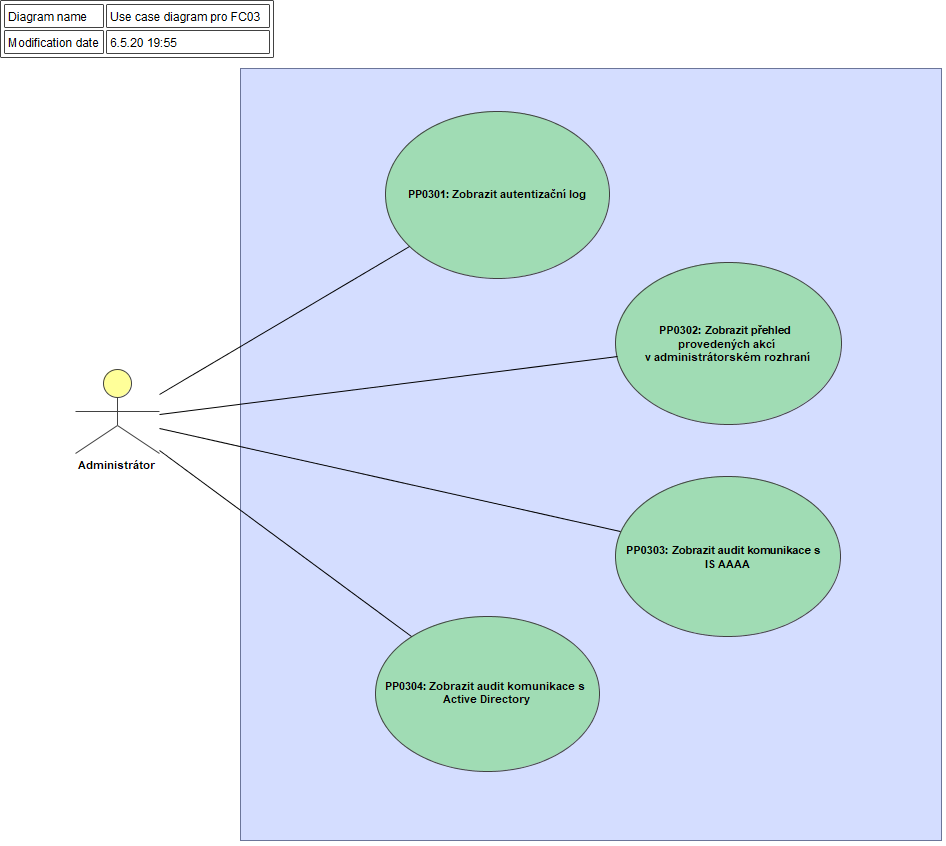
\includegraphics[width=\textwidth]{res/design/Use case diagram pro FC03.png}
  \caption{Funkční celek FC03 a jeho případy použití}
  \label{fig:Funkční celek FC03 a jeho případy použití}
\end{figure}

\newpage
\subsubsection{Případ použití PP0301}
	\begin{longtable}{|g|p{0.80\textwidth}|}
		\hline
		\rowcolor{Blue}\multicolumn{2}{|l|}{\textbf{Zobrazit autentizační log}} \\ \hline
		\textbf{ID případu použití:} & PP0301 \\ \hline
		\textbf{ID požadavku:} & FP0302, FP0301 \\ \hline
		\textbf{Cíl:} & Umožnit přístup k~autentizačnímu logu. \\ \hline
		\textbf{Výchozí podmínky:} & Administrátor má přístup k~serverové části systému. \\ \hline
		\textbf{Uživatel \slash Organizační role:} & Administrátor \\ \hline
		\textbf{Využití služeb jiných systémů:} & \\ \hline
		\textbf{Stav \mbox{po dokončení:}} & Je zobrazen autentizační log. \\ \hline
		\rowcolor{Gray}\multicolumn{2}{|l|}{\textbf{Popis, komentáře}} \\ \hline
		\multicolumn{2}{|p{\textwidth}|}{Tento případ popisuje způsob zobrazení autentizačního logu.} \\ \hline
		\caption{Případ použití PP0301}
		\label{tab:Případ použití PP0301}
	\end{longtable}
	\begin{longtable}{|p{0.07\textwidth}|p{0.93\textwidth}|}
		\rowcolor{Gray}\multicolumn{2}{|l|}{\textbf{Základní scénář}} \\ \hline
		\textbf{Krok} & \\ \hline
		1 & Administrátor spustí průzkumník souborů a vstoupí do adresáře systému s~názvem \texttt{logs}. \\ \hline
		2 & Administrátor pomocí prostředků svého OS zobrazí log \texttt{authentication.log}. \\ \hline
		\caption{Scénář PP0301}
		\label{tab:Scénář PP0301}
	\end{longtable}

\newpage
\subsubsection{Případ použití PP0302}
	\begin{longtable}{|g|p{0.80\textwidth}|}
		\hline
		\rowcolor{Blue}\multicolumn{2}{|l|}{\textbf{Zobrazit přehled provedených akcí v~administrátorském rozhraní}} \\ \hline
		\textbf{ID případu použití:} & PP0302 \\ \hline
		\textbf{ID požadavku:} & FP0302 \\ \hline
		\textbf{Cíl:} & Umožnit přístup k~logu zobrazující přehled provedených akcí v~administrátorském rozhraní. \\ \hline
		\textbf{Výchozí podmínky:} & Administrátor má přístup k~serverové části systému. \\ \hline
		\textbf{Uživatel \slash Organizační role:} & Administrátor \\ \hline
		\textbf{Využití služeb jiných systémů:} & \\ \hline
		\textbf{Stav \mbox{po dokončení:}} & Je zobrazen log přehledu provedených akcí v~administrátorském rozhraní. \\ \hline
		\rowcolor{Gray}\multicolumn{2}{|l|}{\textbf{Popis, komentáře}} \\ \hline
		\multicolumn{2}{|p{\textwidth}|}{Tento případ popisuje způsob zobrazení logu s~přehledem provedených akcí v~administrátorském rozhraní.} \\ \hline
		\caption{Případ použití PP0302}
		\label{tab:Případ použití PP0302}
	\end{longtable}
	\begin{longtable}{|p{0.07\textwidth}|p{0.93\textwidth}|}
		\rowcolor{Gray}\multicolumn{2}{|l|}{\textbf{Základní scénář}} \\ \hline
		\textbf{Krok} & \\ \hline
		1 & Administrátor spustí průzkumník souborů a vstoupí do adresáře systému s~názvem \texttt{logs}. \\ \hline
		2 & Administrátor pomocí prostředků svého OS zobrazí log \texttt{actionsInAdministratorInterface.log}. \\ \hline
		\caption{Scénář PP0302}
		\label{tab:Scénář PP0302}
	\end{longtable}

\newpage
\subsubsection{Případ použití PP0303}
	\begin{longtable}{|g|p{0.80\textwidth}|}
		\hline
		\rowcolor{Blue}\multicolumn{2}{|l|}{\textbf{Zobrazit audit komunikace s~IS~AAAA}} \\ \hline
		\textbf{ID případu použití:} & PP0303 \\ \hline
		\textbf{ID požadavku:} & FP0201 \\ \hline
		\textbf{Cíl:} & Umožnit přístup k~logu zobrazující přehled komunikace s~IS~AAAA. \\ \hline
		\textbf{Výchozí podmínky:} & Administrátor má přístup k~serverové části systému. \\ \hline
		\textbf{Uživatel \slash Organizační role:} & Administrátor \\ \hline
		\textbf{Využití služeb jiných systémů:} & \\ \hline
		\textbf{Stav \mbox{po dokončení:}} & Je zobrazen log s~komunikací s~IS~AAAA. \\ \hline
		\rowcolor{Gray}\multicolumn{2}{|l|}{\textbf{Popis, komentáře}} \\ \hline
		\multicolumn{2}{|p{\textwidth}|}{Tento případ popisuje způsob zobrazení logu s~auditem komunikace s~IS~AAAA.} \\ \hline
		\caption{Případ použití PP0303}
		\label{tab:Případ použití PP0303}
	\end{longtable}
	\begin{longtable}{|p{0.07\textwidth}|p{0.93\textwidth}|}
		\rowcolor{Gray}\multicolumn{2}{|l|}{\textbf{Základní scénář}} \\ \hline
		\textbf{Krok} & \\ \hline
		1 & Administrátor spustí průzkumník souborů a vstoupí do adresáře systému s~názvem \texttt{logs}. \\ \hline
		2 & Administrátor pomocí prostředků svého OS zobrazí log \texttt{communicationLogWithISAAAA.log}. \\ \hline
		\caption{Scénář PP0303}
		\label{tab:Scénář PP0303}
	\end{longtable}

\newpage
\subsubsection{Případ použití PP0304}
	\begin{longtable}{|g|p{0.80\textwidth}|}
		\hline
		\rowcolor{Blue}\multicolumn{2}{|l|}{\textbf{Zobrazit audit komunikace s~Active Directory}} \\ \hline
		\textbf{ID případu použití:} & PP0304 \\ \hline
		\textbf{ID požadavku:} & FP0302 \\ \hline
		\textbf{Cíl:} & Umožnit přístup k~logu zobrazující přehled komunikace s~Active Directory. \\ \hline
		\textbf{Výchozí podmínky:} & Administrátor má přístup k~serverové části systému. \\ \hline
		\textbf{Uživatel \slash Organizační role:} & Administrátor \\ \hline
		\textbf{Využití služeb jiných systémů:} & \\ \hline
		\textbf{Stav \mbox{po dokončení:}} & Je zobrazen log komunikace s~Active Directory. \\ \hline
		\rowcolor{Gray}\multicolumn{2}{|l|}{\textbf{Popis, komentáře}} \\ \hline
		\multicolumn{2}{|p{\textwidth}|}{Tento případ popisuje způsob zobrazení logu s~auditem komunikace s~Active Directory.} \\ \hline
		\caption{Případ použití PP0304}
		\label{tab:Případ použití PP0304}
	\end{longtable}
	\begin{longtable}{|p{0.07\textwidth}|p{0.93\textwidth}|}
		\rowcolor{Gray}\multicolumn{2}{|l|}{\textbf{Základní scénář}} \\ \hline
		\textbf{Krok} & \\ \hline
		1 & Administrátor spustí průzkumník souborů a vstoupí do adresáře systému s~názvem \texttt{logs}. \\ \hline
		2 & Administrátor pomocí prostředků svého OS zobrazí log \texttt{communicationLogWithAD.log}. \\ \hline
		\caption{Scénář PP0304}
		\label{tab:Scénář PP0304}
	\end{longtable}

\subsection{FC04 Autentizace a autorizace}
\label{FC04}
\begin{figure}[H]
  \centering
  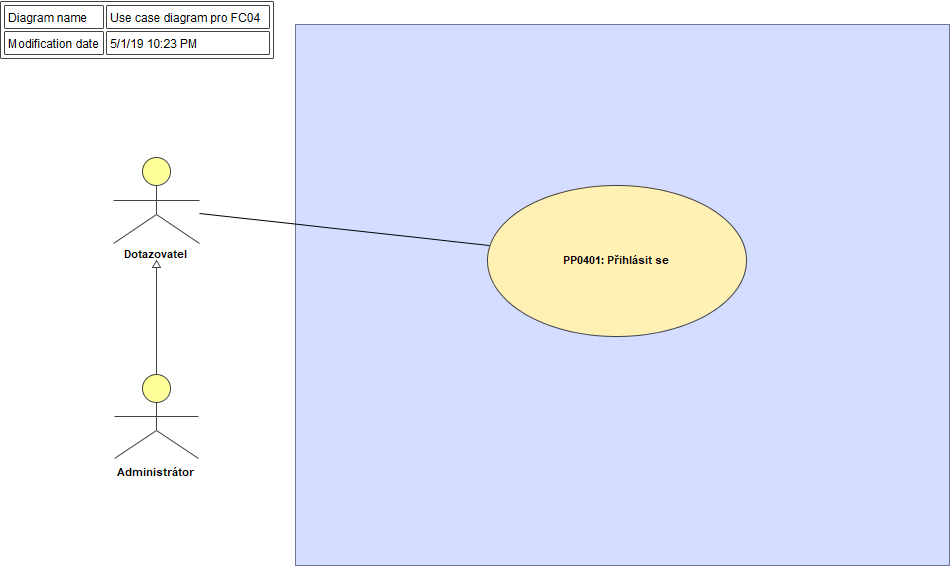
\includegraphics[width=\textwidth]{res/design/Use case diagram pro FC04.png}
  \caption{Funkční celek FC04 a jeho případy použití}
  \label{fig:Funkční celek FC04 a jeho případy použití}
\end{figure}

\newpage
\subsubsection{Případ použití PP0401}
	\begin{longtable}{|g|p{0.80\textwidth}|}
		\hline
		\rowcolor{Blue}\multicolumn{2}{|l|}{\textbf{Přihlásit se}} \\ \hline
		\textbf{ID případu použití:} & PP0401 \\ \hline
		\textbf{ID požadavku:} & FP0301 \\ \hline
		\textbf{Cíl:} & Přihlásit uživatele a zjistit jaké má přiřazené role, od kterých se odvíjí pro něj přístupná funkcionalita. \\ \hline
		\textbf{Výchozí podmínky:} & Q-systém je spuštěn a je možné se k~němu připojit. Active Directory běží v~prostředí zákazníka a je v~ní nadefinován konkrétní uživatel včetně přiřazených rolí. \\ \hline
		\textbf{Uživatel \slash Organizační role:} & Dotazovatel, Administrátor \\ \hline
		\textbf{Využití služeb jiných systémů:} & Rozhraní s~Active Directory \\ \hline
		\textbf{Stav \mbox{po dokončení:}} & Uživatel je přihlášen, jsou známé jeho role, a tudíž i formy dotazu, které může použít. Jsou zneplatněné typy entit, na které uživatel nemá oprávnění se dotazovat. \\ \hline
		\rowcolor{Gray}\multicolumn{2}{|l|}{\textbf{Popis, komentáře}} \\ \hline
		\multicolumn{2}{|p{\textwidth}|}{Tento případ popisuje sled aktivit probíhající během a po přihlášení uživatelů do systému. Informace o~tom, že uživatel má administrátorské oprávnění je rovněž v~Active Directory.} \\ \hline
		\caption{Případ použití PP0401}
		\label{tab:Případ použití PP0401}
	\end{longtable}
\newpage
	\begin{longtable}{|p{0.07\textwidth}|p{0.93\textwidth}|}
		\rowcolor{Gray}\multicolumn{2}{|l|}{\textbf{Základní scénář}} \\ \hline
		\textbf{Krok} & \\ \hline
		1 & Uživatel se pomocí prohlížeče přihlásí na URL, na kterém je systém vystaven. \\ \hline
		2 & Uživatel nerozeznán, je vyžadována autentizace. \\ \hline
		3 & Uživatel zadá své přihlašující údaje, tedy \textit{login} a heslo. \\ \hline
		4 & Systém deleguje autentizaci na Active Directory. \\ \hline
		5 & Active Directory uživatele úspěšně autentizuje. \\ \hline
		6 & Systém zaloguje úspěšné přihlášení do \hyperref[Logy]{autentizačního logu}. \\ \hline
		7 & Systém se dotáže Active Directory na všechny přiřazené role pro daného uživatele. \\ \hline
		8 & Systém zaloguje komunikaci s~Active Directory do \hyperref[Logy]{audit logu komunikace s~Active Directory}. \\ \hline
		9 & Systém má nyní seznam uživatelských rolí a bude tvořit seznam forem dotazu. Pro každou roli v~konfiguračním souboru najde, jaké formy dotazu tato role povoluje, a přidá je do seznamu forem dotazu pro daného uživatele (bez duplicit). \\ \hline
		10 & Na základě seznamu uživatelových povolených forem dotazu systém definuje průnik těchto forem, aby získal přehled o~všech možných kombinacích typů dotazu, modifikátorů dotazu a typů entit. \\ \hline
		11 & Systém v~\hyperref[RozbalovaciMenu]{rozbalovacím menu} zobrazí nabízenou funkcionalitu pro daného uživatele. Zobrazeny budou typy entit, na které uživatel má oprávnění se dotazovat na základě průniku forem dotazu.
Pokud má uživatel zároveň roli Administrátora, budou mu navíc zobrazeny možnosti administrace systému. \\ \hline
		\rowcolor{Gray}\multicolumn{2}{|l|}{\textbf{Alternativní scénáře}} \\ \hline
		\textbf{Krok} & \\ \hline
		2a &
		2a1 Uživatel je rozeznán jako již autorizavaný.
		
  		2a2 Pokračuje se krokem 6 základního scénáře. \\ \hline
  		5a &
		5a1 Autentizace uživatele skončí neúspěšně.
		
  		5a2 Systém zaloguje pokus o~přihlášení do \hyperref[Logy]{autentizačního logu}.
  		
  		5a3 Systém zaloguje komunikaci s~Active Directory do \hyperref[Logy]{audit logu komunikace s~Active Directory}.
  		
  		5a4 Systém zobrazí informaci o~neúspěšné autentizaci. \\ \hline
  		9a & Systém zná přiřazené uživatelské role z~Active Directory, ve které ovšem jsou také role se systémem nijak nesouvisející. Pokud je přidána nová role určená pro systém do Active Directory, může se stát, že bylo opomenuto přidat ji také do systému. Systém upozorní uživatele, že má přiřazené role, které jsou pro systém neznámé. Pokud mají být použity, nejprve musí Administrátor aktualizovat seznam definovaných rolí ručním přidáním rolí do systému, viz \hyperref[PP0202]{PP0202}. \\ \hline
  		\caption{Scénář PP0401}
		\label{tab:Scénář PP0401}
	\end{longtable}

\subsection{Transformace odpovědi na dotaz typu \textit{Doplňující dotaz}}
\label{cqrd}
Pokud je v~odpovědi na dotaz typu \textit{Základní dotaz} přiřazená nějaká vazba na připojený záznam, lze se na něj dotázat doplňkovým dotazem typu \textit{Doplňující dotaz}, který vrací odlišnou stromovou strukturu. Tato struktura obsahuje všechny informace, jaké by obsahovala i odpověď na dotaz typu \textit{Základní dotaz}, tyto informace jsou ovšem odlišně strukturované.  Aby bylo možné zobrazit připojený záznam ve stejné struktuře jako byly zobrazeny záznamy v~odpovědi na dotaz typu \textit{Základní dotaz}, definoval jsem transformaci odpovědi na dotaz typu \textit{Doplňující dotaz} na odpoveď na dotaz typu \textit{Základní dotaz}.

Kvůli anonymizaci jsem popis této transformace odstranil. Ovšem, jak jsem tuto transformaci technicky provedl popíšu v~podkapitole \hyperref[Transf]{Transformace odpovědi na dotaz typu \textit{Doplňující dotaz}}.

Následuje návrh uživatelského rozhraní s~návrhy obrazovek, které, na základě mého textového popisu, vytvořil kolega Tomáš Trapl. Do práce jsem je zahrnul, protože do návrhu logicky patří.

\section{Uživatelské rozhraní a výstupy}
\subsection{O01 Úvodní obrazovka a menu}
\begin{figure}[H]
  \centering
  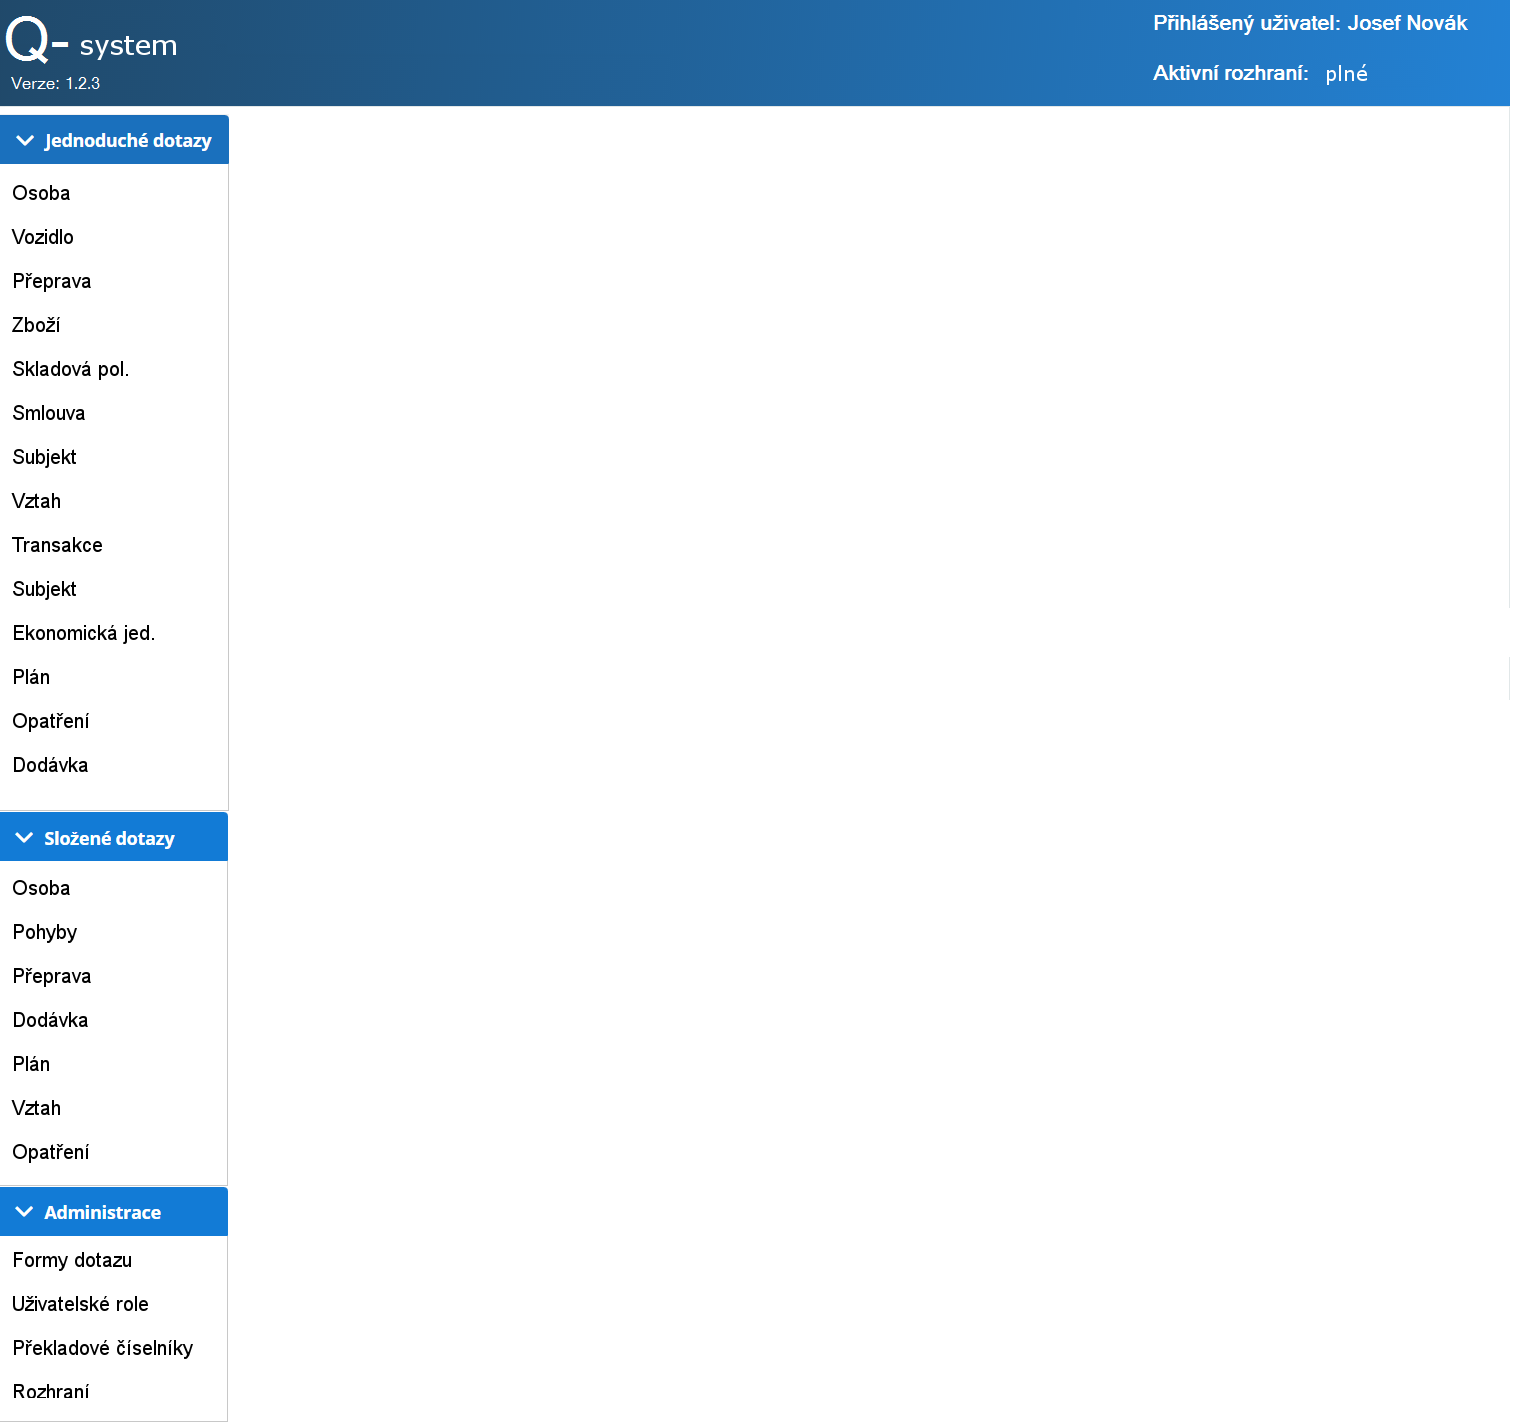
\includegraphics[width=\textwidth]{res/screens/O01 Úvodní obrazovka a menu.png}
  \caption{O01 Úvodní obrazovka}
  \label{fig:O01 Úvodní obrazovka}
\end{figure}

\label{HorniLista}
Základ aplikace tvoří horní lišta s~názvem aplikace, ve které je uvedena aktuální verze aplikace, údaje o~přihlášeném uživateli a o~aktuálně používaném rozhraní.

V~jednotlivých funkcích bude poté pod horní lištou uvedena navigační lišta (tzv. \textit{breadcrumb}) zobrazující, v~jaké funkci se uživatel nachází (viz další obrazovky).

\label{RozbalovaciMenu}
V~levé části je rozbalovací menu, které obsahuje všechny funkce dostupné přihlášenému uživateli podle rolí, které má přiřazené v~Active Directory. Na obrázku je znázorněna maximální možná nabídka funkcí.

\subsection{O02 Dotaz}
\label{O02Dotaz}
\begin{figure}[H]
  \centering
  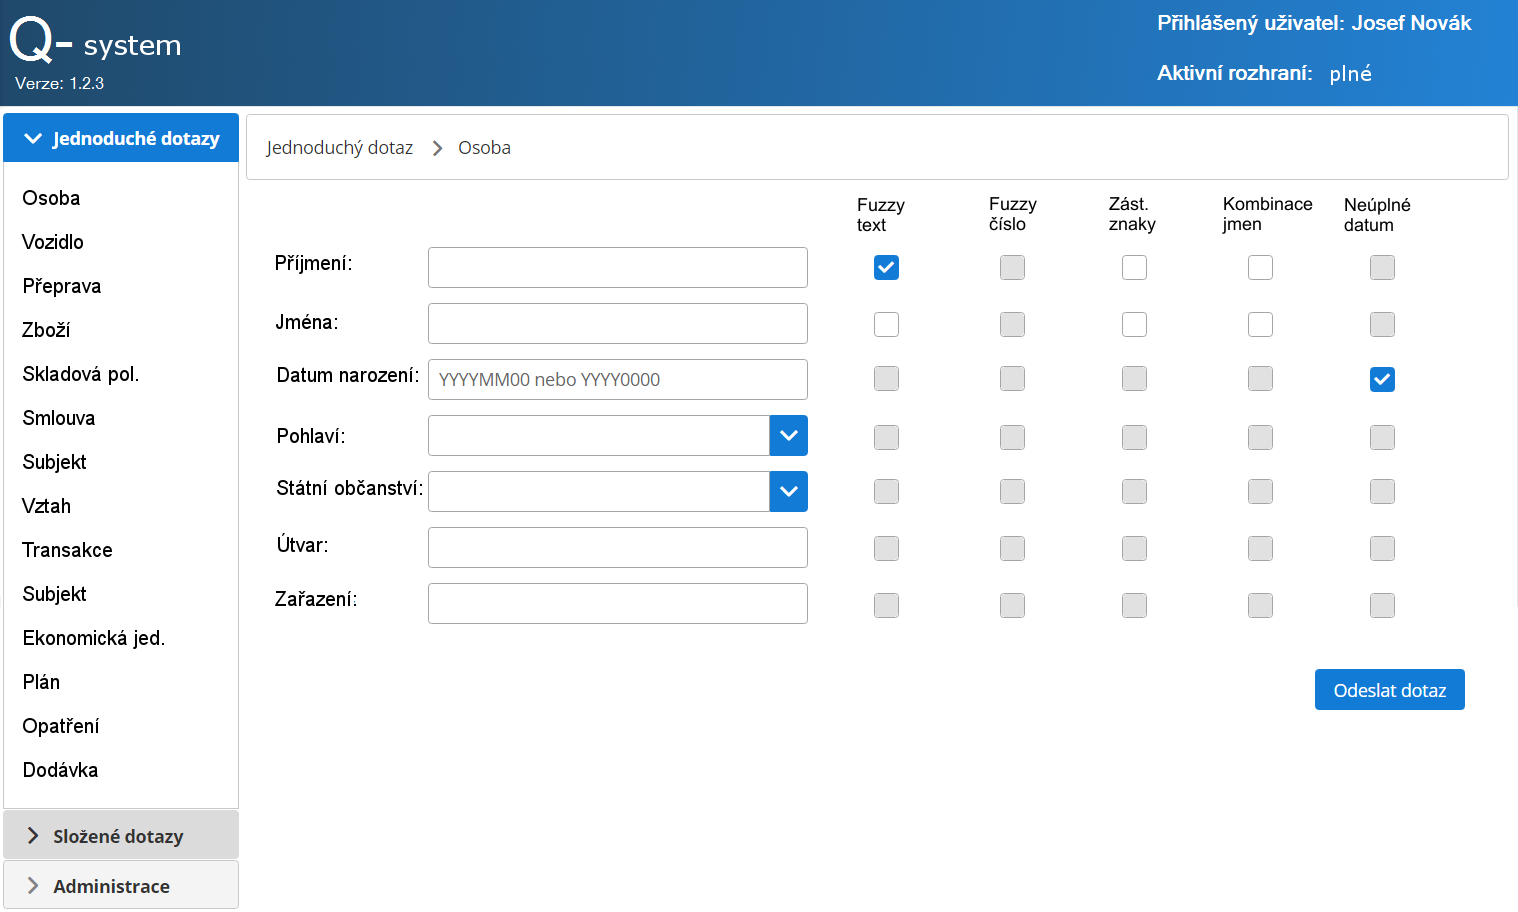
\includegraphics[width=\textwidth]{res/screens/O02 Dotaz.png}
  \caption{O02 Dotaz}
  \label{fig:O02 Dotaz}
\end{figure}

Aplikace při použití funkce pro položení dotazu zobrazí odpovídající vyhledávací kritéria a nastaví pro ně povolené modifikátory (zpřístupní je nebo znepřístupní). V~poli pro zadání hodnoty kritéria jsou ve složitějších případech uvedeny nápovědy na požadovaný formát hodnoty.

Uživatel vyplní vybraná kritéria, vybere pro ně požadované modifikátory a potvrdí dotaz pomocí tlačítka \uv{Odeslat dotaz}. Pokud nebudou hodnoty některých kritérií korektní, aplikace zobrazí chyby validace.

U~kritérií s~nabídkou hodnot (zde \uv{Pohlaví} a \uv{Státní občanství}) bude možné vyhledávat\slash navigovat v~seznamu nabízených hodnot a hodnoty budou setříděné abecedně. Tato kritéria nabízejí číselníkové hodnoty dle \hyperref[Logy]{konfigurace překladových číselníků}. Musí zobrazovat uživatelský překlad, originální ICT název a kód, např: Červená -- Red -- XXXX.YY.

Kritérium státní občanství je výčtového typu ICT006\_Narodnost. Budou zachovány všechny nabízené státy dle oficiálního ICT číselníkového dokumentu \cite{ICT}, ve kterém jsou ovšem některé státy, například Súdán, vícekrát (verze 01\slash02). Je potřeba zachovat možnost dotazovat se i na starší Súdán, jehož platnost zadání již vypršela. GUI graficky od sebe odliší platné a neplatné záznamy.


\subsection{O03 Odpověď na dotaz}
\label{O03OdpovedNaDotaz}
\begin{figure}[H]
  \centering
  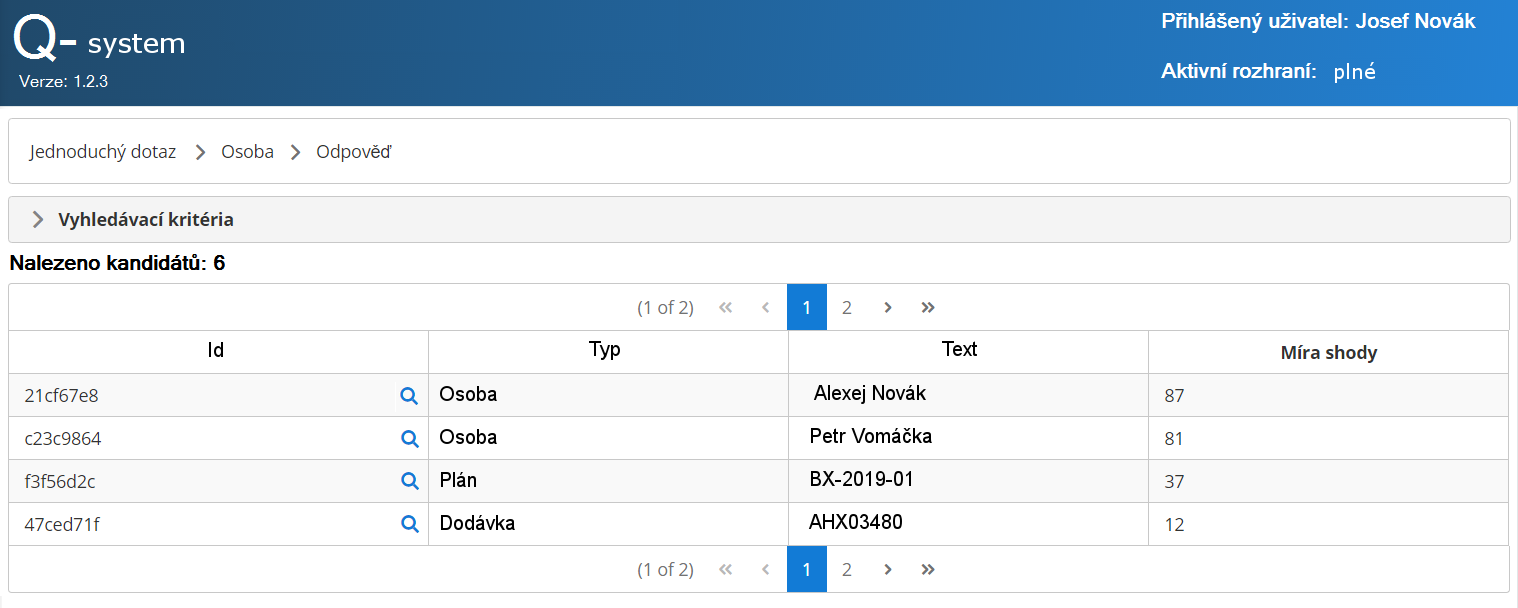
\includegraphics[width=\textwidth]{res/screens/O03 Odpověď na dotaz.png}
  \caption{O03 Odpověď na dotaz}
  \label{fig:O03 Odpověď na dotaz}
\end{figure}

Aplikace zobrazuje odpověď na dotaz do nové záložky prohlížeče. Aplikace zobrazí pod navigační lištou sbalený panel s~výběrovými kritérii (obsah je stejný jako při zadávání dotazu, pouze jsou všechna pole neaktivní a nelze měnit jejich obsah).

Dále aplikace zobrazí počet nalezených kandidátů a tabulku s~těmito kandidáty. Pokud počet kandidátů přesáhne nastavený limit pro jednu stránku (doporučeno 10 záznamů), budou další zobrazeny na stránkách 2, 3 atd. Stránkování a navigace po stránkách bude zobrazena v~tabulce nahoře i dole pro snadnou dostupnost.

Uživatel si může zobrazit detail vybraného kandidáta pomocí tlačítka s~lupou v~příslušném řádku (viz \hyperref[O04DetailKandidata]{O04 Detail kandidáta}).

\subsection{O04 Detail kandidáta}
\label{O04DetailKandidata}
\begin{figure}[H]
  \centering
  \includegraphics[width=\textwidth]{res/screens/O04 Detail kandidáta.png}
  \caption{O04 Detail kandidáta}
  \label{fig:O04 Detail kandidáta}
\end{figure}

Aplikace zobrazuje každý detail kandidáta na novou záložku prohlížeče.

Údaje o~kandidátovi jsou rozděleny do tří panelů:
\begin{itemize}
	\item Metadata -- technické a doprovodné údaje o~nalezeném kandidátovi
	\item Osobní údaje\slashÚdaje o~objektu -- popisné údaje nalezeného kandidáta
	\item Doplňkové údaje -- seznam identifikátorů doplňkových údajů, které je možné pro kandidáta získat
\end{itemize}

Každý panel bude možné samostatně sbalit nebo rozbalit.

Při použití tlačítka s~lupou v~doplňkových údajích aplikace získá a zobrazí tento údaj na nové záložce prohlížeče (tlačítko bude k~dispozici pouze u~údajů, které lze zobrazit). Při použití tlačítka s~lupou v~záhlaví \uv{Doplňkové údaje} aplikace získá všechny doplňkové údaje, které lze zobrazit a zobrazí je na samostatných nových záložkách prohlížeče.

Při použití tlačítka se symbolem uložení v~doplňkových údajích aplikace zobrazí standardní \textit{save dialog} pro uložení souboru s~tímto údajem (tlačítko bude k~dispozici pouze u~údajů, které má smysl ukládat do souboru).

Aplikace bude poskytovat následující typy doplňkových údajů s~uvedenými operacemi:
\begin{itemize}
	\item Doplňující informace -- zobrazení údaje
	\item Přílohy -- zobrazení i uložení údaje
	\item Vazby -- zobrazení i uložení údaje
\end{itemize}

\subsection{O05 Formy dotazu}
\label{O05FormyDotazu}
\begin{figure}[H]
  \centering
  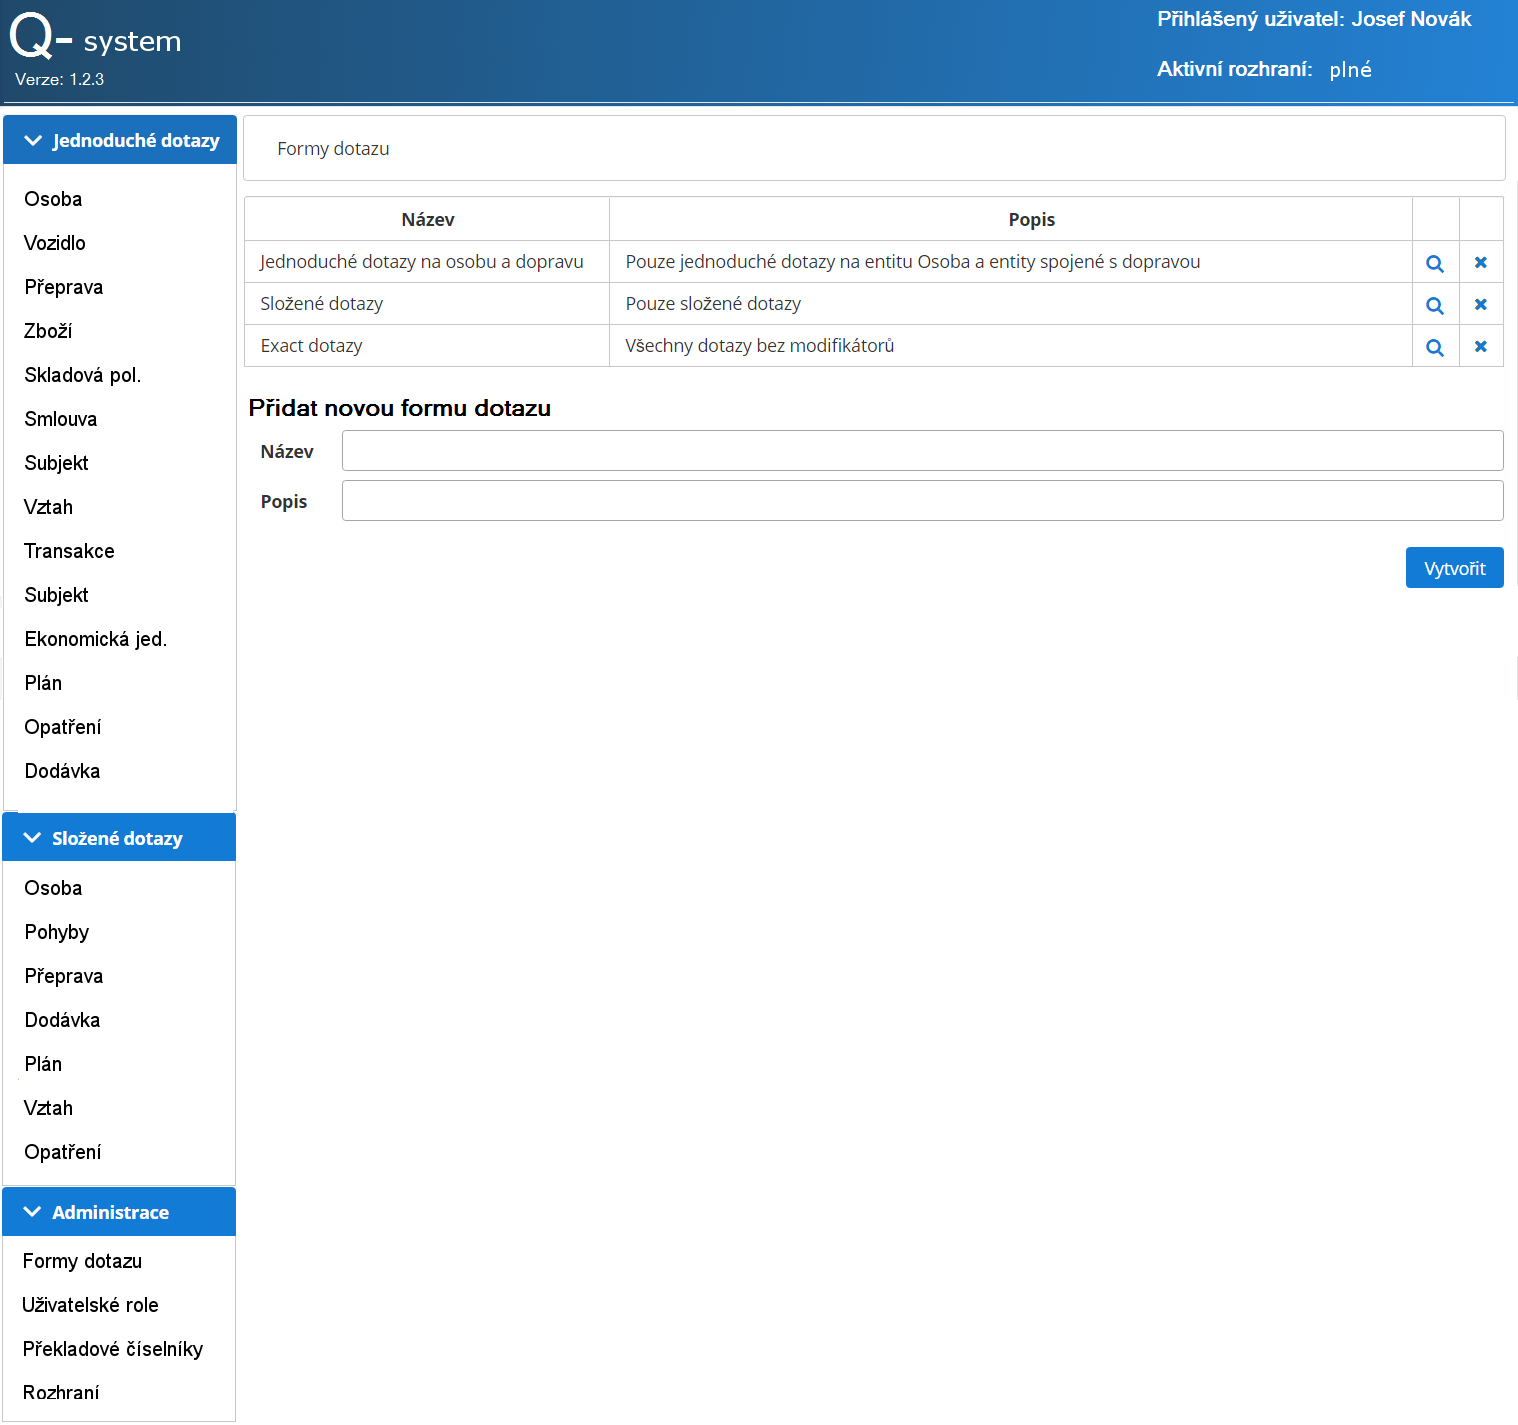
\includegraphics[width=\textwidth]{res/screens/O05 Formy dotazu.png}
  \caption{O05 Formy dotazu}
  \label{fig:O05 Formy dotazu}
\end{figure}

Aplikace zobrazí seznam existujících forem dotazu.

Použitím tlačítka s~lupou v~příslušném řádku uživatel otevře detail definice vybrané formy dotazu (viz \hyperref[O06FormaDotazuDetail]{O06 Forma dotazu – detail}).

Použitím tlačítka s~křížkem v~příslušném řádku uživatel zruší vybranou formu dotazu. Aplikace zobrazí potvrzovací dotaz \uv{Skutečně chcete zrušit vybranou formu dotazu?}. Pokud uživatel zrušení potvrdí, aplikace ověří, že vybranou formu dotazu nemá přiřazenou žádná uživatelská role. Pokud je forma dotazu přiřazena nějaké roli, aplikace zobrazí chybu. Pokud není forma přiřazena, aplikace smaže její definici a aktualizuje zobrazený seznam forem dotazu.

Uživatel může vytvořit novou formu dotazu zadáním názvu a popisu do polí pod seznamem existujících forem. Uživatel potvrdí založení nové formy použitím tlačítka \uv{Vytvořit}. Aplikace ověří, že neexistuje jiná forma se stejným názvem, a pokud ano, zobrazí chybu. Pokud je název nové formy unikátní, aplikace ji vytvoří a zobrazí její detail (viz \hyperref[O06FormaDotazuDetail]{O06 Forma dotazu – detail}).

\subsection{O06 Forma dotazu -- detail}
\label{O06FormaDotazuDetail}
\begin{figure}[H]
  \centering
  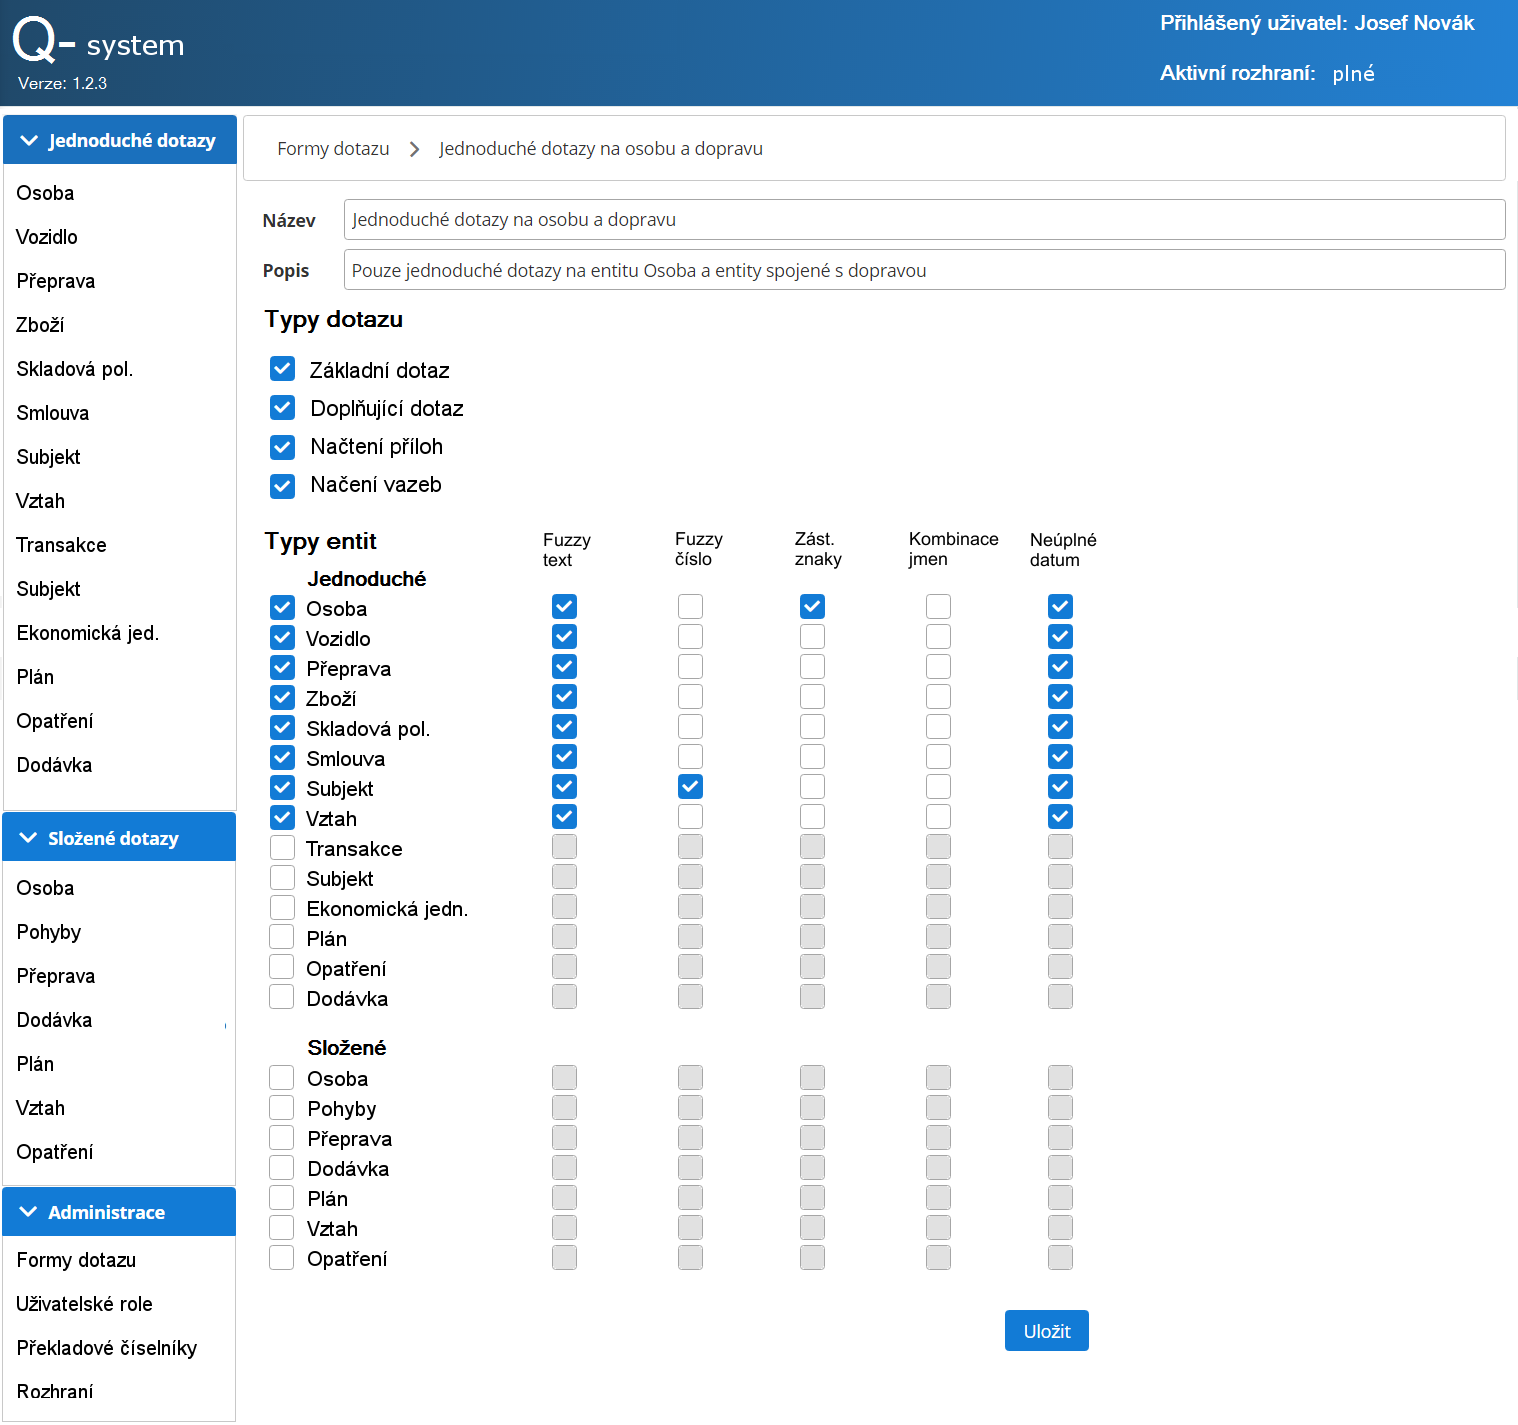
\includegraphics[width=\textwidth]{res/screens/O06 Forma dotazu - detail.png}
  \caption{O06 Forma dotazu -- detail}
  \label{fig:O06 Forma dotazu -- detail}
\end{figure}

Uživatel zaškrtne typy dotazu, které bude moci držitel této formy provádět.

Uživatel zaškrtne typy entit, které bude moci držitel této formy použít, a pro každý vybraný typ entity specifikuje množinu povolených modifikátorů dotazu.

Pomocí tlačítka \uv{Uložit} potvrdí uživatel definici zobrazené formy dotazu a aplikace tuto definici uloží.

\subsection{O07 Uživatelské role}
\label{O07UzivatelskeRole}
\begin{figure}[H]
  \centering
  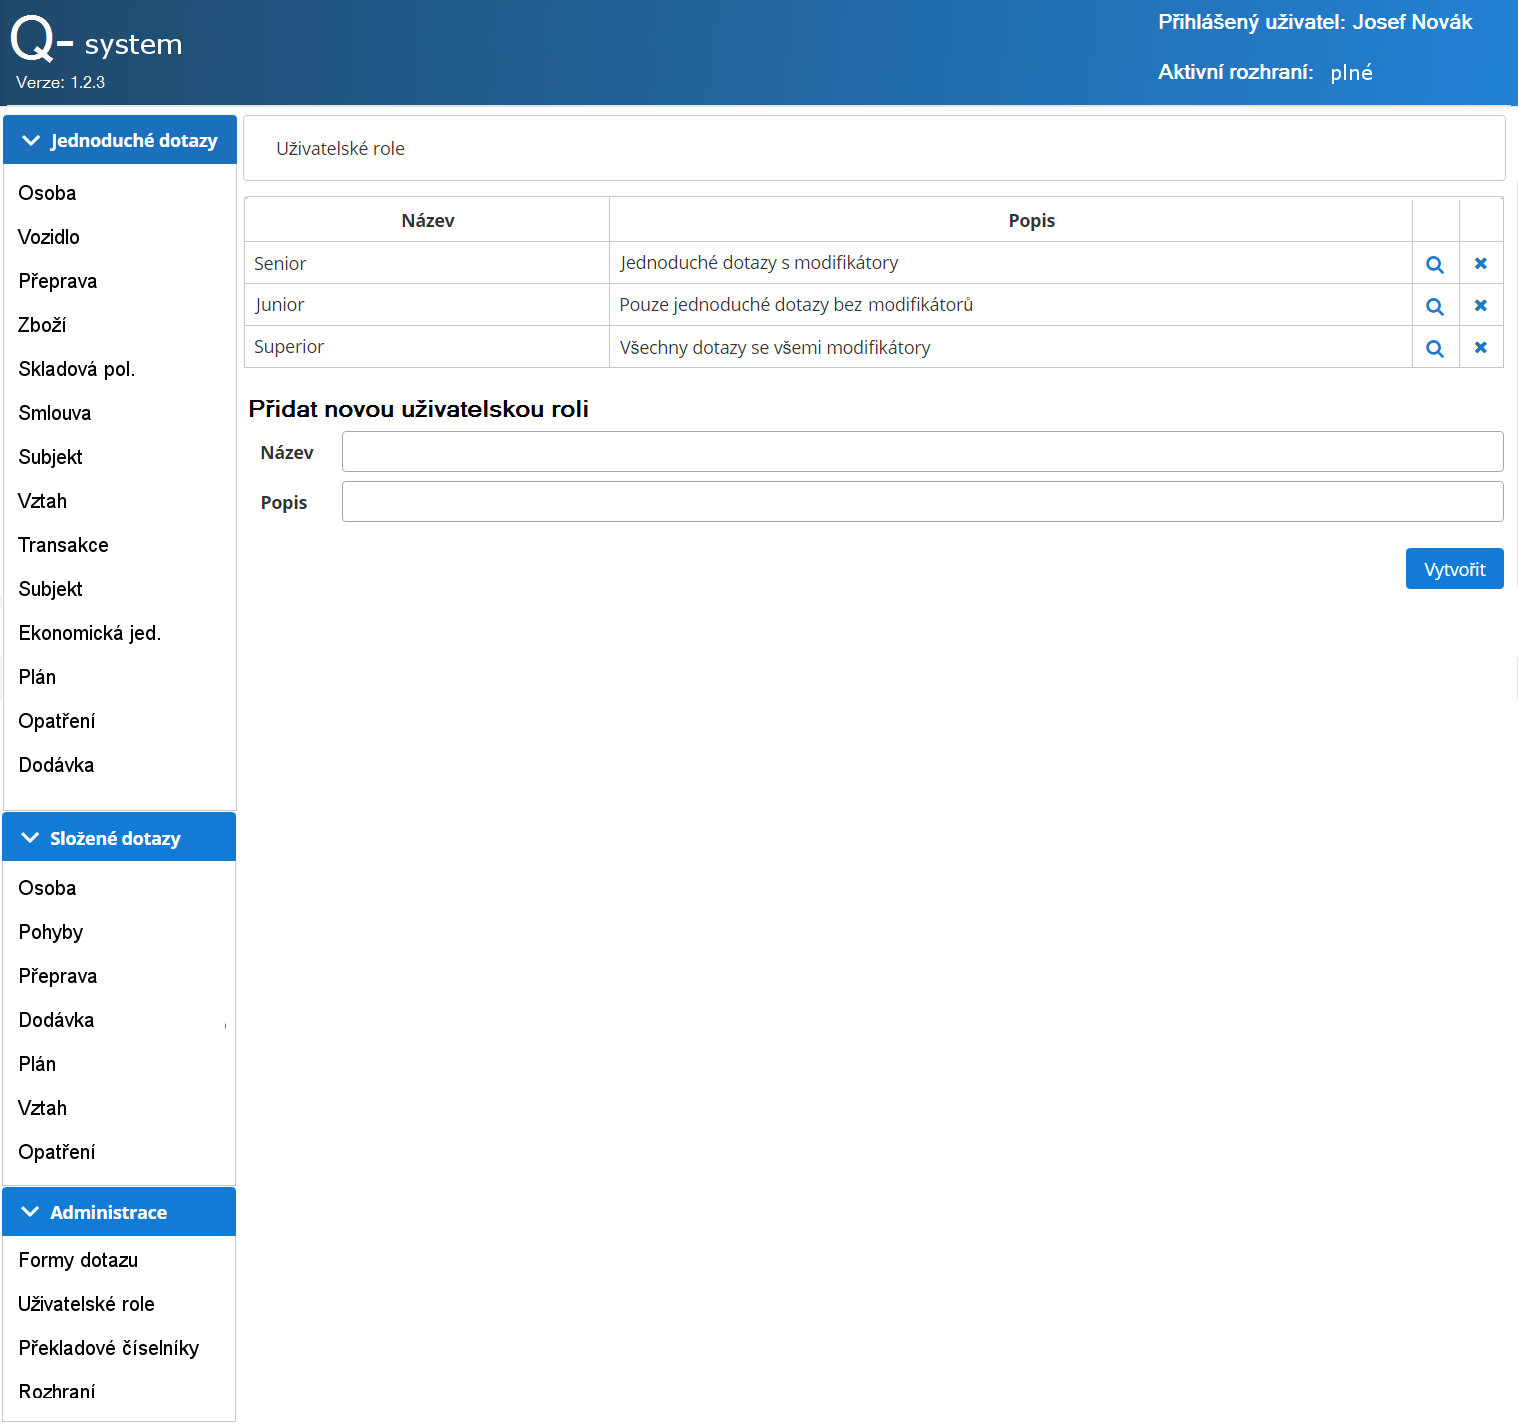
\includegraphics[width=\textwidth]{res/screens/O07 Uživatelské role.png}
  \caption{O07 Uživatelské role}
  \label{fig:O07 Uživatelské role}
\end{figure}

Aplikace zobrazí seznam existujících uživatelských rolí.

Použitím tlačítka s~lupou v~příslušném řádku uživatel otevře detail definice vybrané uživatelské role (viz \hyperref[O08UzivatelskaRoleDetail]{O08 Uživatelská role – detail}).

Použitím tlačítka s~křížkem v~příslušném řádku uživatel zruší vybranou uživatelskou roli. Aplikace zobrazí potvrzovací dotaz \uv{Skutečně chcete zrušit vybranou formu dotazu?}. Pokud uživatel zrušení potvrdí, aplikace smaže definici vybrané role a aktualizuje zobrazený seznam rolí.

Uživatel může vytvořit novou uživatelskou roli zadáním názvu a popisu do polí pod seznamem existujících rolí. Uživatel potvrdí založení nové role použitím tlačítka \uv{Vytvořit}. Aplikace ověří, že neexistuje jiná uživatelská role se stejným názvem, a pokud ano, zobrazí chybu. Pokud je název nové role unikátní, aplikace ji vytvoří a zobrazí její detail (viz \hyperref[O08UzivatelskaRoleDetail]{O08 Uživatelská role – detail}).

\subsection{O08 Uživatelská role -- detail}
\label{O08UzivatelskaRoleDetail}
\begin{figure}[H]
  \centering
  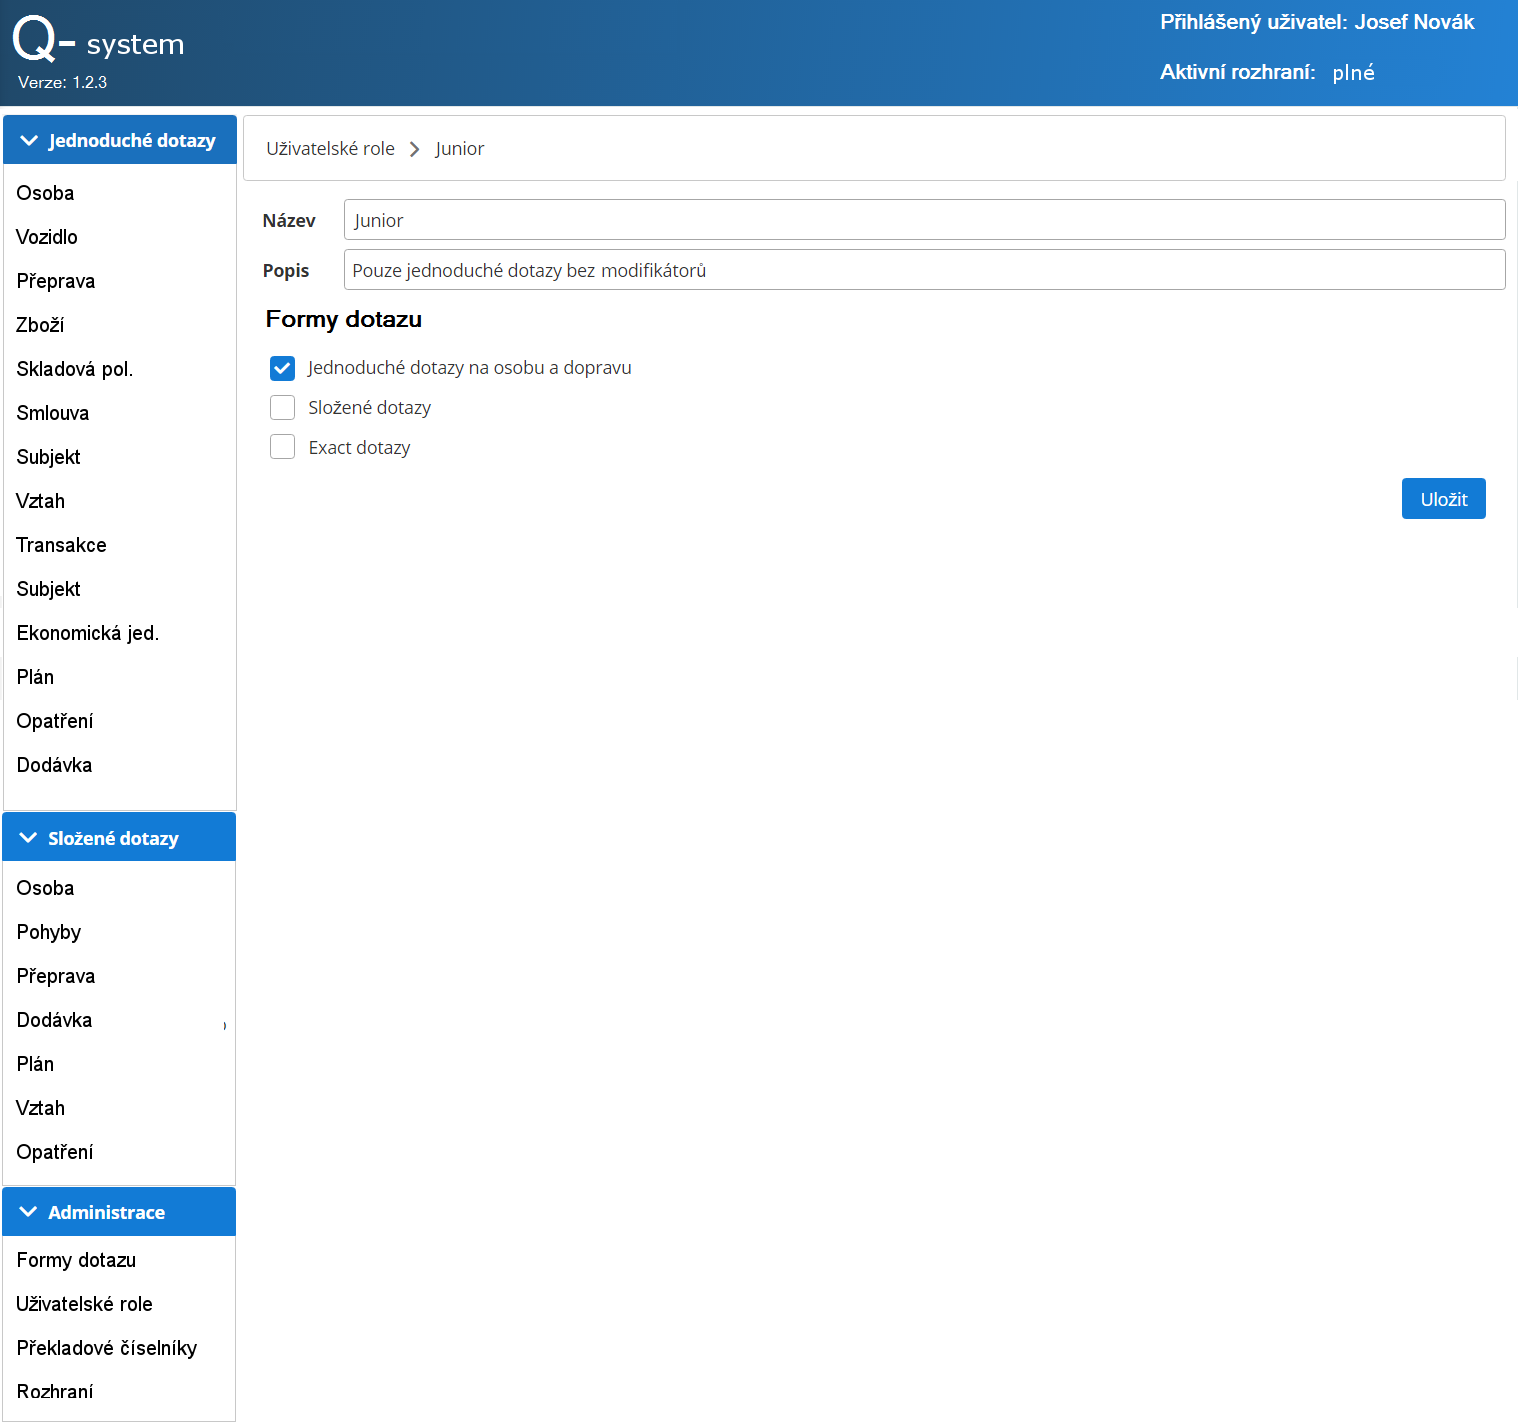
\includegraphics[width=\textwidth]{res/screens/O08 Uživatelská role - detail}
  \caption{O08 Uživatelská role -- detail}
  \label{fig:O08 Uživatelská role -- detail}
\end{figure}

Uživatel zaškrtne formy dotazu, které chce přiřadit definované roli.

Pomocí tlačítka \uv{Uložit} potvrdí uživatel definici zobrazené uživatelské role a aplikace tuto definici uloží.

\subsection{O09 Překladové číselníky}
\label{O09PrekladoveCiselniky}
\begin{figure}[H]
  \centering
  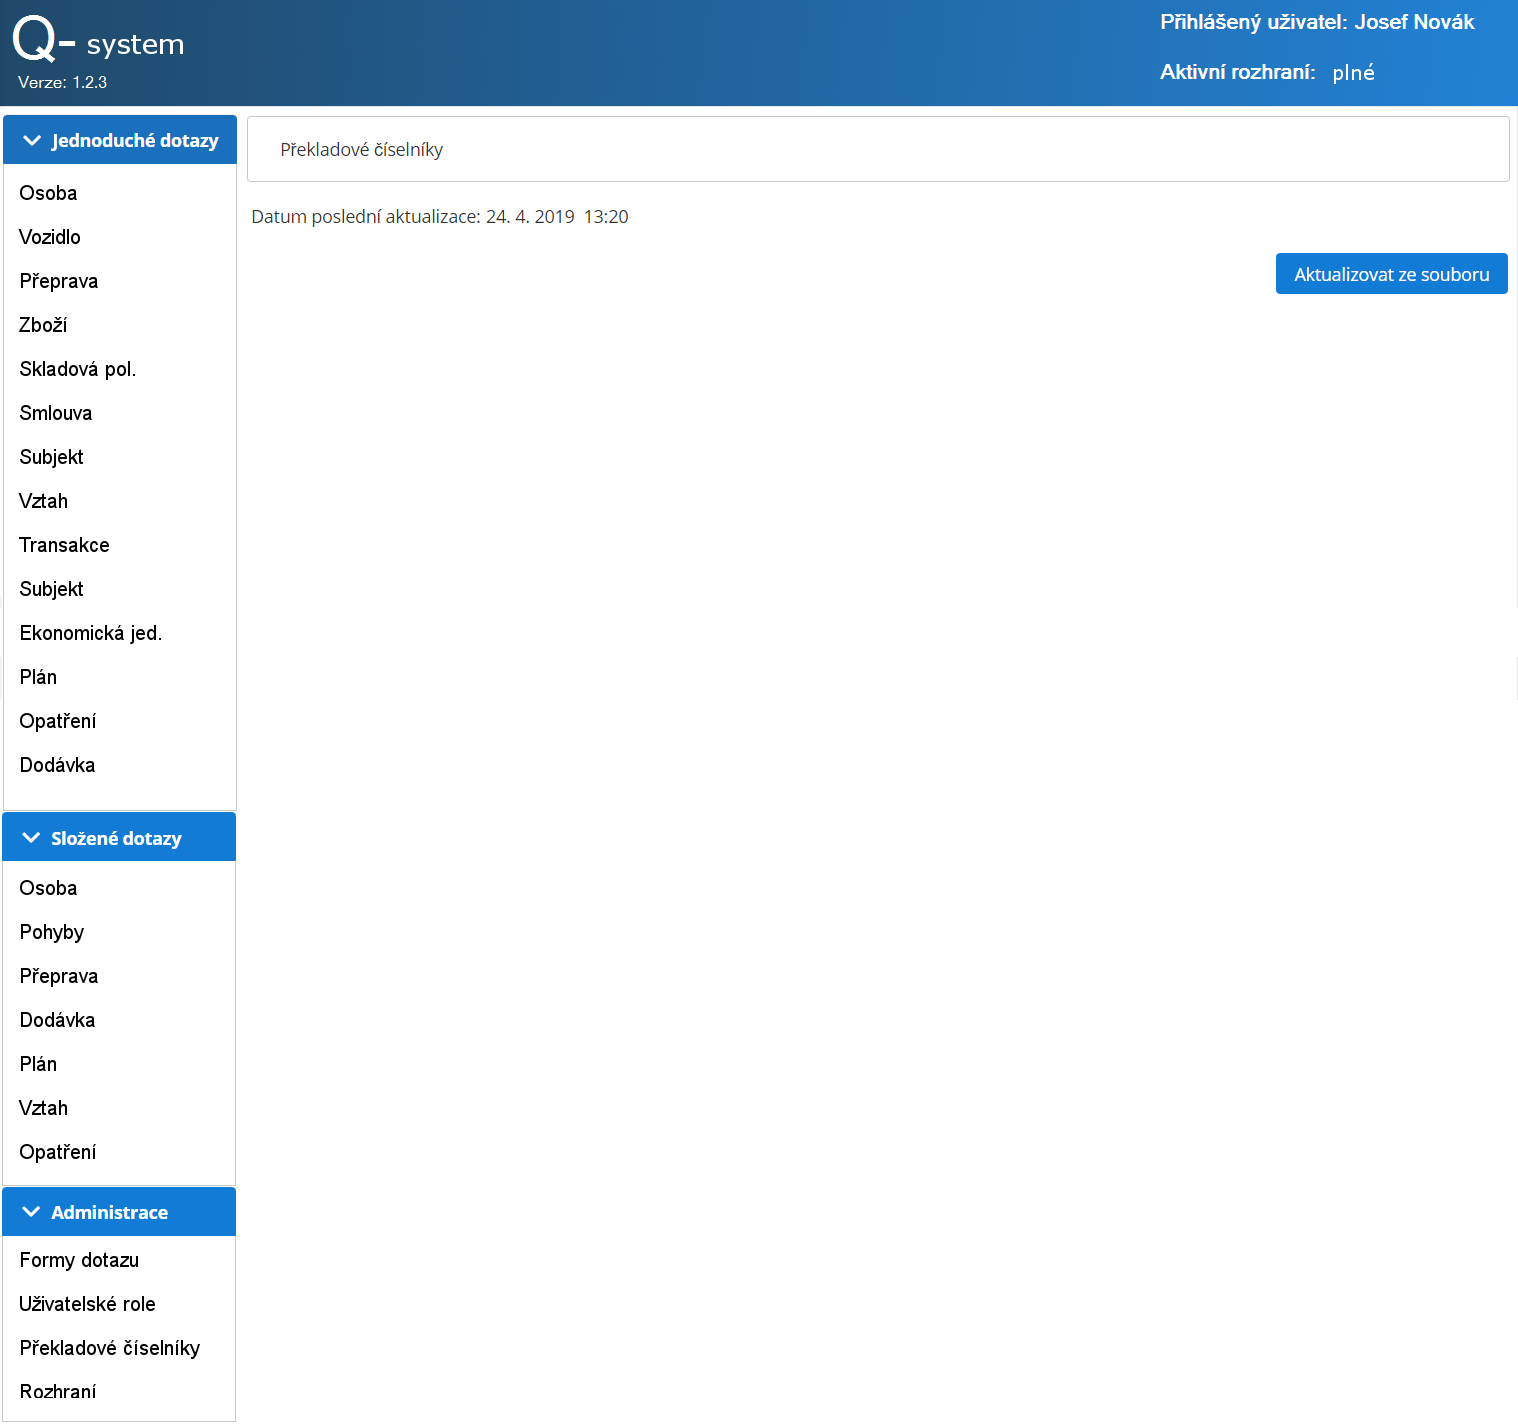
\includegraphics[width=\textwidth]{res/screens/O09 Překladové číselníky.png}
  \caption{O09 Překladové číselníky}
  \label{fig:O09 Překladové číselníky}
\end{figure}

Aplikace zobrazuje datum a čas poslední úspěšné aktualizace překladových číselníků.

Pomocí tlačítka \uv{Aktualizovat ze souboru} aplikace spustí standardní \textit{open dialog} a uživatel v~něm vybere soubor, ze kterého chce číselníky aktualizovat.

Aplikace provede aktualizaci a její výsledek zobrazí buď jako informaci o~úspěšném provedení, nebo jako chybu.

\subsection{O10 Rozhraní na IS~AAAA}
\label{O10RozhraniNaISAAA}
\begin{figure}[H]
  \centering
  \includegraphics[width=\textwidth]{res/screens/O10 Rozhraní na IS AAAA.png}
  \caption{O10 Rozhraní na IS~AAAA}
  \label{fig:O10 Rozhraní na IS~AAAA}
\end{figure}

Aplikace zobrazuje preferované rozhraní (nastavené konfiguračně) a aktuálně používané rozhraní (nastavené aplikačními mechanismy).

Pomocí tlačítka \uv{Změnit} u~preferovaného rozhraní uživatel vynutí změnu preferovaného rozhraní na IS~AAAA (viz \hyperref[O11ZmenaRozhraniNaISAAA]{O11 Změna rozhraní na IS~AAAA}).

Pomocí tlačítka \uv{Nastavit na preferované} uživatel vyvolá změnu aktuálně používaného rozhraní na rozhraní nastavené jako preferované.

\newpage
\subsection{O11 Změna rozhraní na IS~AAAA}
\label{O11ZmenaRozhraniNaISAAA}
\begin{figure}[H]
  \centering
  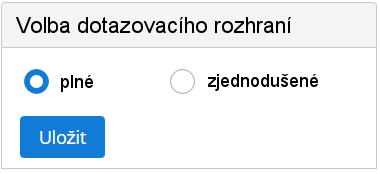
\includegraphics[scale=0.75]{res/screens/O11 Změna rozhraní na IS AAAA.png}
  \caption{O11 Změna rozhraní na IS~AAAA}
  \label{fig:O11 Změna rozhraní na IS~AAAA}
\end{figure}

Aplikace zobrazí dialogové okno pro volbu rozhraní.

Uživatel označí rozhraní, které chce nastavit jako preferované, a potvrdí volbu tlačítkem \uv{Uložit}. Aplikace uloží vybrané rozhraní do konfigurace a zavře dialogové okno. Následně aktualizuje zobrazené údaje o~rozhraní (viz \hyperref[O10RozhraniNaISAAA]{O10 Rozhraní na IS~AAAA}).

\newpage
\section{Specifikace HW architektury}
\subsection{Schéma HW architektury}
\begin{figure}[H]
  \centering
  \includegraphics[width=\textwidth]{res/design/Diagram nasazení.png}
  \caption{Diagram nasazení}
  \label{fig:Diagram nasazení}
\end{figure}

Na základě nefunkčních požadavků z~analýzy (zejména PV03 a PV04) bude použita architektura klient -- server. Q-systém bude dodán dle požadavku PV04 jako webová aplikace skládající se ze serverové části a tenkého klienta. Tenkým klientem je libovolné zařízení s~webovým prohlížečem.

Serverová část poskytuje prohlížečům obrazovky GUI přes HTTPS protokol. Jedná se o~samostatnou aplikaci, která běží na cílové platformě CentOS (dle \hyperref[NefunkcniPozadavky]{PV01}). Funkčnost serverové části je podmíněna jejím správným napojením na Active Directory a IS~AAAA.

\subsection{Distribuce}
Q-systém je v~první podobě distribuován jako samostatný \textit{jar} soubor. Obsahem souboru je zabalený projekt včetně všech použitých knihoven. Z~hlediska terminologie Spring Bootu se jedná o~tzv. \uv{\textit{fat-jar}}, který při spuštění nejprve nastartuje zabudovaný aplikační server Tomcat, nasadí Q-systém a zpřístupní jej na předem definovaném URL a portu. \cite{FatJar}

Apache Tomcat byl vybrán, protože je \textit{open-source} a protože se jedná o~suverénně nejpopulárnější aplikační server. Každoročně jeho podíl na trhu roste, v~roce 2017 ho používalo přes 63 \% trhu. \cite{ApplicationServers}

Nutno podotknout, že volba konkrétního Java aplikačního serveru není definitivní a je snadné zabudovaný Tomcat vyměnit, například za Eclipse Jetty. Formálně vzato, označit Tomcat jako aplikační server není zcela přesné, nepodporuje EJB nebo distribuované transakce. Je to spíše webový server, který ale navíc slouží jako \textit{servlet} kontejner, tudíž poskytuje běhové prostředí pro \textit{servlety}, technologie JSP \& JSF, díky kterým dokáže generovat také dynamický obsah, na rozdíl od klasického webového serveru. \cite{Tomcat}

Drobnou změnou konfigurace, Spring Boot dokáže vyprodukovat místo \textit{jar} souboru, \textit{war} soubor. Pokud to bude v~budoucnosti žádoucí, bude možné jednoduše nasadit Q-systém ve formě \textit{war} souboru na již existující aplikační server.

\newpage
\section{Návrh SW architektury}
Jak již naznačila předchozí kapitola, byla zvolena klient -- server architektura. Jednotlivé vrstvy architektury budou probrány v~následujících kapitolách.

\subsection{Výběr frameworků}
Na následujícím obrázku jsou znázorněny vybrané frameworky a jejich umístění do jednotlivých architektonických vrstev. Tato práce se zabývá pouze aplikační a perzistentní vrstvou.

\begin{figure}[H]
  \centering
  \includegraphics[width=\textwidth]{res/design/SW architektura Q-systému.png}
  \caption{Výběr frameworků}
  \label{fig:Výběr frameworků}
\end{figure}

\subsection{Backend}
\subsubsection{Aplikační vrstva}
Na základě požadavku na podporu Linuxu, dostupnosti \textit{frameworků} a osobní preference byl pro implementaci backendové části zvolen objektově orientovaný jazyk Java. 
Konkrétně \textit{open-source} \textit{release} Open JDK 11.0.2. Java 11 je LTS verze s~veřejnou podporou do září 2022. \cite{JavaHistory, OpenJDK}

Bude využit robustní Spring Framework verze 5.1, který je součástí Spring Bootu verze 2.1.4. Spring Boot slouží k~auto-konfiguraci Springu a zrychluje vývoj díky heslu: \uv{\textit{convention over configuration}}.

\subsubsection{Perzistentní vrstva}
Z~analýzy Q-systému vyplynulo, že aplikace nepotřebuje používat žádnou databázi. Dotaz sestavený v~aplikaci je předán do IS~AAAA a synchronně je zobrazena odpověď. Není potřeba ukládat stav odeslaného požadavku. Přidat databázi by mělo smysl, kdyby se v~budoucnosti uvažovalo rozšířit Q-systém, aby dokázal administrátorovi zobrazit nějaké statistiky a přehledy odeslaných požadavků z~nějakého období. Taková funkcionalita ovšem pro verzi 1.0.0. požadována nebyla.

Aplikace si vystačí s~konfiguračními soubory. Tyto soubory budou stejně jako logovací soubory uloženy na serverové části Q-systému. Cílem je, aby ležely fyzicky mimo výslednou aplikaci, a bylo tak možné konfiguraci měnit bez nutnosti \textit{re-buildu} celé aplikace.

Jedná se tedy o~dvouvrstvou architekturu, protože aplikační a perzistentní vrstva leží na stejném hardwaru.
Prezentační vrstva běží v~prohlížeči u~klienta.

\newpage
\lbparagraph{Konfigurace Q-systému}
\label{Konfigurace}
Po zvolení konfiguračních souborů vznikla otázka, v~jakém formátu budou informace uloženy. Jako první mě napadl JSON, který je stručnější a pro lidi lépe čitelný, než XML. 

Po provedení rešerše jsem pochopil, proč JSON není vhodný jazyk pro konfiguraci: \cite{JSON}
\begin{itemize}
	\item absence komentářů -- JSON byl vytvořen za účelem přenosu dat
	\item nepodporuje víceřádkové řetězce
	\item striktní syntaxe -- má výhodu lehkého parsování, ovšem snižuje čitelnost
	\item mnoho speciálních symbolů -- například pokud je klíč identifikátor a hodnota číslo, potom jsou povinné uvozovky kolem číselné hodnoty redundantní
\end{itemize}
Tyto nedostatky odstraňuje stále populárnější jazyk TOML, proto jsem ho vybral jako formát  dat pro uložení konfigurace Q-systému. \cite{TOML}

\begin{lstlisting}[frame=single,caption=Příklad jazyka TOML,label=TomlExample]
# This is a TOML document.

title = "TOML Example"

multilinestr = """
Roses are red
Violets are blue"""

[owner]
name = "Tom Preston-Werner"
dob = 1979-05-27T07:32:00-08:00 # First class dates

[database]
server = "192.168.1.1"
ports = [ 8001, 8001, 8002 ]
connection_max = 5000
enabled = true
\end{lstlisting}

\newpage
Konfigurace Q-systému je uložena napříč více konfiguračními soubory:
\begin{enumerate}
	\item \texttt{authorization.toml}
	
	Konfigurační soubor ve formátu TOML, který spravuje:
	\begin{itemize}
		\item seznam definovaných uživatelských rolí
		\item seznam definovaných forem dotazu
		\item mapování uživatelských rolí na formy dotazu
	\end{itemize}

	\item \texttt{interface.toml}
	
	Konfigurační soubor ve formátu TOML, který obsahuje:
	\begin{itemize}
		\item aktuálně používané rozhraní IS~AAAA
		\item preferované rozhraní IS~AAAA
	\end{itemize}

	\item \texttt{translationDials.toml}
	
	Překladové číselníky budou uloženy v~konfiguračním souboru, který bude obsahovat klíče (zobrazované v~GUI) a jim odpovídající hodnoty, kterým rozumí IS~AAAA.

	Při pokládání dotazu typu \textit{Základní dotaz} lze specifikovat různá kritéria. Některá jsou výčtového typu a jejich konkrétní hodnoty budou převzaty z~ICT číselníků \cite{ICT}. Konfigurační soubor Q-systému s~překladovými číselníky tudíž musí spravovat tyto ICT číselníky:
	\label{PrekladoveCiselniky}
	\begin{itemize}
	\item ICT001\_TypDotazovatele
	\item ICT002\_TypZaznamu
	\item ICT006\_Narodnost
	\item ICT012\_ZnackaVozu
	\item ICT013\_Barva
	\item ICT017\_TypTransakce
	\item ICT018\_TypEkonomickeJednotky
	\item ICT021\_TypOpatreni
	\item ICT022\_TypPlanu
	\item ICT024\_TypSubjektu
	\item ICT025\_TypSmlouvy
	\item ICT026\_TypSkladovePolozky
	\item ICT029\_TypVazby
	\item ICT031\_ZpusobTransakce
	\item ICT108\_KombinaceModifikatoru
	\item ICT129\_Pohlavi
	\item ICT130\_ZpusobVazby
	\end{itemize}
	Názvy klíčů překladových číselníků ovšem může Administrátor změnit nahráním vlastního upraveného konfiguračního souboru s~překladovými číselníky, viz \hyperref[PP0204]{PP0204}.
\end{enumerate}

\lbparagraph{Logy\\}
\label{Logy}
Pro logování byl vybrán projekt Logback. Jedná se o~následníka Log4J.

Logovat se bude do těchto 4 souborů:
\begin{itemize}
	\item \texttt{authentication.log} (autentizační log)
	\item \texttt{actionsInAdministratorInterface.log} (log provedených akcí v~administrátorském rozhraní)
	\item \texttt{communicationLogWithISAAAA.log} (audit log komunikace s~IS~AAAA)
	\item \texttt{communicationLogWithAD.log} (audit log komunikace s~Active Directory)
\end{itemize}

Případně je možné logovat nějaké události také na konzoli.
Logback umožňuje definovat různé \textit{layouty} specifikující formátování zpráv.

\subsection{Frontend}
Po návrhu obrazovek vyvstala otázka, jestli je potřeba SPA\slash MPA webová aplikace.

Q-systém nenabízí extrémně bohaté GUI s~mnoha funkcemi, které by měly dynamicky měnit vzhled stránky.  Programování na straně klienta je minimální, proto lze vykonat \textit{business} logiku, a rovnou \textit{vyrenderovat} stránky, na straně serveru. Stačí synchronní bezestavová komunikace s~okolními systémy. Je tedy zvolena \textit{multiple page} aplikace. Její výhodou je možnost použití tenkých klientů s~webovým prohlížečem bez podpory Javascriptu. Každá stránka má vlastní URL, tudíž vyhledávače mohou stránky snadno indexovat a provádět SEO. \cite{SPAvsMPA, DontNeedSPA}

\subsubsection{Prezentační vrstva}
Java poskytuje více technologií pro tvorbu uživatelského rozhraní MPA webových aplikací: JSP nebo JSF. 
JSF je MVC webový \textit{framework} podporující mapování grafických komponent na tzv. \textit{backing beans} a používání \textit{servletových} kontrolerů. Jedná se o~modernější přístup než JSP, proto byla vybrána technologie JSF. \cite{JSPvsJSF}

Jedná se o~specifikaci, která má více implementací. Jedna z~nich je \textit{open-source} a jmenuje se Primefaces. Primefaces nabízí řadu předpřipravených komponent, které budou využity při tvorbě GUI. \cite{Primefaces}

\subsection{Licence}
Při výběru technologií byl kladen důraz po požadavek \hyperref[NefunkcniPozadavky]{PV01}. Všechny technologie tak mají nějakou formu \textit{open-source} licence. \cite{OpenSourceLicence}
\begin{itemize}
	\item OpenJDK: GNU General Public License, version 2, with the Classpath Exception
	\item Spring Boot: Apache License 2.0
	\item Spring: Apache License 2.0
	\item Primefaces: Apache License 2.0
\end{itemize}

\subsection{Autentizace}
\subsubsection{Autentizace uživatelů Q-systému}
Q-systém se skládá ze serverové části (\textit{stateful} server) a klientských webových prohlížečů, komunikující se serverem přes HTTPS protokol. Uživatelé Q-systému se autentizují vůči externímu LDAP serveru (Active Directory).

\subsubsection{Autentizace vůči IS~AAAA}
Q-systém se musí při posílání dotazu autentizovat platným certifikátem vůči IS~AAAA -- to je vlastností IS~AAAA. Distribuce certifikátů je součástí nutné konfigurace při instalaci Q-systému v~prostředí zákazníka.

\subsubsection{Rozhraní externích systémů}
Q-systém komunikuje s~2 externími systémy: IS~AAAA a Active Directory. Tato komunikace je vždy synchronní.

Z~integračního pohledu se jedná o~\textit{One-to-One Service Integration}.

\chapter{Realizace}
\label{Realizace}
V~této kapitole popíšu, jaké možnosti návrhu a implementace jsem zvažoval, a zmíním zajímavé problémy, které jsem při programování musel vyřešit.

\section{Práce na projektu}
\label{PraceNaProjektu}
Úvodní zájem o~dotazovací systém přišel od zadavatele začátkem února roku 2019. Téma mě zaujalo, začal jsem tedy s~vedoucím práce sestavovat formální zadání, abych mohl projekt použít i jako svou diplomovou práci.

Bylo potřeba se vymezit, co bude mým dílem. Od začátku jsem věděl, že se chci zaměřit hlavně na analýzu, návrh a implementaci backendu. Bylo tedy domluveno, že frontend implementuje kolega Tomáš Novák. 
Z~tohoto důvodu jsem se vyhnul také grafickému návrhu uživatelských obrazovek, které, na základě mého textového popisu, vytvořil kolega Tomáš Trapl. Do práce jsem je zahrnul, protože do návrhu logicky patří.

Ostatní je mým dílem. Ve finále jsem značně vypomáhal i na frontendu, protože jsem vybral technologii JSF, která je úzce spojená s~Javou. Využívá kontrolery, které jsou napsané v~Javě. Až na drobné úpravy lze tedy souhrnně říci, že všechny Java soubory jsou mým dílem a kolega Tomáš Novák vytvořil zejména \texttt{.xhtml} šablony, které následně nastyloval pomocí \texttt{.css} souborů.

Práce na projektu začala 20. 2. 2019 úvodní schůzkou, na které jsem si upřesnil se zadavatelem většinu požadavků kladených na systém. 

Dále bylo nutné nastudovat interní popisy systému IS~AAAA \cite{IsAAA, i1, i2}, se kterým Q-systém komunikuje, a také možné typy dotazů, které umožňuje centrální systém IS~AAAB položit. \cite{Queries, ICT}. Zohledněním těchto zdrojů jsem vytvořil analytickou část, to byla náplň března 2019.

V~dubnu jsem sestavoval návrhový dokument, včetně pozdějšího rozplánování implementace na jednotlivé podúlohy, včetně jejich odhadů pracnosti. Zároveň jsem, po vybrání technologií, v~polovině dubna, prováděl \textit{Proof of concept}, jehož snahou bylo dokázat, že vybrané technologie lze použít společně. K~tomuto tématu se vrátím v~následující kapitole.

Od května 2019 začal vývoj. V~polovině čevna se ke mně přidal kolega Tomáš Novák a začal paralelně pracovat na frontendu. V~červenci jsem programoval nejintenzivněji, protože jsem vypomáhal na frontendu a chtěl jsem backend kompletně dodělat, než odletím na výměnný pobyt do zahraničí. To se mi podařilo.

Finalizace frontendu probíhala bez mé přítomnosti od srpna do začátku září 2019, kdy byl produkt úspěšně akceptován a předán zadavateli. 

\begin{itemize}
	\item Spočítal jsem, že jsem vytvořil přes 8 200 řádek Java kódu, které jsem rozdělil do 123 tříd\slash rozhraní.
	\item Mimo to jsem také autorem souboru \texttt{app-features.xml}, který vytahuje informace z~interního wordovského dokumentu Queries Description a obsahuje 5 000 řádek. Q-systém tento soubor pouze čte. \cite{Queries}
	\item Dále jsem vytvořil výchozí konfigurační soubor \texttt{traslationDials.toml}, který kopíruje vytažené údaje z~interního excelu ICT Code Tables. \cite{ICT}
	\item XHTML šablony bez CSS mají pro představu skoro 3 000 řádek.
\end{itemize}

\section{Implementace}
\subsection{Proof of concept a bean scopes} 
Ukázalo se, že použít JSF uvnitř Spring Boot aplikace není úpně standardní. Z~několika \textit{hello-world} tutoriálů jsem si vybral jeden funkční z~webu \\\url{codenotfound.com}. \cite{CodeNotFound}

Tento základ spoléhá na knihovnu JoinFaces, která umožňuje použití Primefaces (JSF) uvnitř Spring Boot aplikace. JSF jakožto \textit{framework} umožňuje vytvářet tzv. \textit{beany}, které v~aplikaci vzniknou za běhu, nějakou dobu žijí a poté zanikají. Rozsah platnosti \textit{beany} se nazývá \textit{scope}. Spring Boot je postaven nad \textit{frameworkem} Spring, který rovněž spoléhá na své vlastní \textit{beany}. Problémem je, že \textit{scopy} JSF \textit{bean} jsou odlišné než \textit{scopy} Spring \textit{bean} nebo nemají stejný rozsah platnosti. Je potřeba tedy vybrat, jaké \textit{bean scopy} se mají používat. Odlišný je také DI mechanismus. Toto je podstatná věc, kterou knihovna JoinFaces rovněž řeší, a to tak, že preferuje springovský CDI s~tím, že přidává neduplicitní JSF \textit{scopy}, např. \uv{\textit{View}}. \cite{ManagedBeans, CDI, JSFDI}

Používal jsem tedy klasické CDI anotace, jako \texttt{@Named}, \texttt{@Inject} atd. Anotace pro definici \textit{bean scope} byly jak CDI, tak JSF, například: \cite{JoinFaces}
\begin{itemize}
	\item \texttt{@javax.enterprise.context.ApplicationScoped}
	\item \texttt{@javax.enterprise.context.SessionScoped}
	\item \texttt{@javax.enterprise.context.RequestScoped}
	\item \texttt{@javax.faces.bean.ViewScoped}
\end{itemize}

Výchozí \textit{scope} je \textit{singleton}. 

Později jsem narazil, když jsem se snažil získat pomocí DI mechanismu referenci buď na \texttt{@RequestScoped} nebo  \texttt{@SessionScoped} \textit{beanu} uvnitř \textit{singleton} \textit{beany}. Jedná se o~známý problém, který řeší například \\ interface \texttt{javax.inject.Provider}. \cite{InjectIntoSingletonBean}

\subsection{Grafová reprezentace formy dotazu}
Formu dotazu tvoří jednotlivé kombinace typu dotazu, typu entity a modifikátoru dotazu, například \textit{Základní dotaz}, \textit{Osoba}, \textit{Fuzzy text}. Taková kombinace umožní dotazovateli položit standardní dotaz na osoby a navíc specifikovat modifikátor \textit{Fuzzy text} u~vyhledávacích kritérií, například u~příjmení. Nastavením příjmení na \uv{Nová} s~aktivním modifikátorem \textit{Fuzzy text}, by IS~AAAA mohl najít jak záznam s~\uv{Novákem}, tak s~\uv{Nováčkem}. Pokud by byl oproti tomu dotaz položen s~modifikátorem \textit{Přesná hodnota} u~příjmení, potom by byly vráceny záznamy pouze s~příjmením odpovídající přesně řetězci \uv{Nová}. \cite{Queries}

Dotazovací rozhraní nabízí velmi širokou množinu možností. Bylo potřeba najít mechanizmus, který by kontroloval, které kombinace jsou pro dotazovatele zpřístupněny dle jeho přiřazených forem dotazu. Formu dotazu jsem se rozhodl v~aplikaci reprezentovat jako tripartitní graf, který zajišťuje, že tato kontrola je efektivní. Průnik forem dotazu  tedy získám průnikem tripartitních grafů.
 
Tripartitní graf je takový graf, jehož množinu vrcholů je možné rozdělit na tři disjunktní množiny (tzv. parity) tak, že žádné dva vrcholy ze stejné množiny nejsou spojeny hranou. Tyto tři parity jsou v~mém případě tedy:
\begin{enumerate}
	\item Typy dotazu
	\item Typy entit
	\item Modifikátory dotazu
\end{enumerate}

\subsection{JAX-WS a generování mapovaných JAXB Java tříd pro odeslání dotazu}
JAX-WS je standardizované API pro komunikaci pomocí SOAP webových služeb. Toto API bylo zvolené pro komunikaci se systémem IS~AAAA. Dle existujícího WSDL popisu webových služeb se při \textit{buildu} vygenerují potřebné Java třídy, díky kterým sestavení dotazu znamená jen správné vytvoření a naplnění odpovídajících objektů. Jedná se o~tzv. \textit{top-down} přístup. \cite{JaxWS}

V~mém projektu jsou v~současnosti dva WSDL soubory, jeden pro rozhraní \textit{Plné rozhraní} a druhý popisující \textit{Zjednodušené rozhraní}. Rozhraní \textit{Plné rozhraní} nabízí více metod. Oba WSDL soubory se odkazují do XSD definicí. Protože na rozhraní \textit{Zjednodušené rozhraní} lze potenciálně zakrývat části odpovědi od IS~AAAA, je většina elementů z~odpovídající XSD definice volitelná.

Mapované Java třídy jsou vygenerovány příkazem \texttt{wsimport} do\\ \texttt{target/generated-sources/isaaa-request-wsimport}.
IS~AAAA nabízí bohaté dotazovací rozhraní, proto odpovídající XSD definují mnoho typů, a~z~toho důvodu se generuje několik Java tříd:
\begin{itemize}
	\item 102 tříd odpovídajících balíčku \texttt{cz.komix.isaaa.query}
	\item 615 tříd odpovídajících balíčku \texttt{ANONYMIZED}
\end{itemize}

Na základě vložených informací na frontendu aplikace vytvoří odpovídající Java objekty, které se serializují (\textit{JAXB marshalling}) do formátu XML  a následně jsou přes JAX-WS odeslány formou SOAP zprávy do IS~AAAA.

\subsection{Generování mapovaných JAXB Java tříd pro odpověď od IS~AAAA}
Příchozí textovou odpověď od IS~AAAA je vhodné ověřit oproti nějaké očekávané struktuře. Taková struktura je popsaná XSD souborem \\ \texttt{ISAAAQueryResponseMessages.xsd}. 

Podobně, jako při konfiguraci příkazu \texttt{wsimport} v~předchozí části, bylo i~zde potřeba (v~\texttt{pom.xml}) nastavit generování mapovaných JAXB Java tříd pro odpověď. \cite{JAXB}
Toho bylo docíleno příkazem \texttt{xjc}. Vygenerované soubory jsou ve složce\\ \texttt{target/generated-sources/isaaa-response-xjc} a obsahují:
\begin{itemize}
	\item 223 tříd odpovídajících balíčku \texttt{cz.komix.isaaa.query.response}
\end{itemize}

Generovaní tříd zpomaluje \textit{build}. Abych omezil počet generovaných tříd, namapoval jsem odpovědi do jednotné struktury, ať už přišly z~jakékoholiv rozhraní. Například odpověď na dotaz typu \textit{Základní dotaz} se namapuje na objekt \textit{odpoveď na dotaz typu Základní dotaz}, který se již následně posílá z~backendu na frontend k~zobrazení dotazovateli.

\subsection{Transformace odpovědi na dotaz typu \textit{Doplňující dotaz}}
\label{Transf}
Při analýze struktury odpovědi na dotaz typu \textit{Doplňující dotaz} (viz \ref{cqrd}) jsem zjistil, že téměř nijak nerozšiřuje strukturu odpovědi na dotaz typu \textit{Základní dotaz} (v~případě, kdybychom se na stejnou entitu dotázali dotazem typu \textit{Základní dotaz}). Data jsou jen odlišně strukturovaná. Abych ušetřil práci na frontendu, rozhodl jsem se, vytvořit mapování struktury odpovědi \textit{Doplňujícího dotazu} na odpoveď \textit{Základního dotazu}.

V~původním návrhu jsem předpokládal XLST transformaci, která by pozměnila XML odpověď \textit{Doplňujícího dotazu} na XML odpověď \textit{Základního dotazu}. To jsem nakonec zavrhl, protože jsem našel jednodušší cestu, a to místo složitého popisu XLST transformace použít XML DOM Parser. \cite{DOMParser}

\subsection{Thread-safety}
Před \textit{refactoringem} jsem se vrátil k~rozboru částí kódu, které nebyly \textit{thread-safe} a hrozily \textit{race conditions}. Některé potenciálně problematické metody, jako například transformaci z~předchozího bodu, jsem prošel a následně označil za bezestavové, tudíž automaticky \textit{thread-safe}. Tam, kde více vláken přistupuje ke sdíleným proměnným, jsem musel použít zamykání pomocí synchronizovaných metod nebo bloků kódu (např. v~metodě \texttt{setPreferredISAAAInterface}). \cite{ThreadSafety}

Nevynechal jsem ani prověření klíčových externích knihoven. Při \textit{marshallingu} se vytváří \textit{marshaller} z~JAXB kontextu, který je sám o~sobě \textit{thread-safe}, \textit{marshaller} již nikoliv. \cite{JAXBThreadSafe}
Pro každé rozhraní IS~AAAA je tedy vytvořen vlastní JAXB kontext, ze kterého vznikne \textit{marshaller} a \textit{unmarshaller}. 

Bohužel se ukázalo, že ani odesílání dotazu pomocí JAX-WS není \textit{thread-safe}. 
Řešení jsem navrhl tak, že každý dotaz vytvoří vlastní \texttt{@RequestScoped} objekt \texttt{ISAAAQueryServicesProxy}, který teprve používá \texttt{@WebServiceRef} anotaci. \cite{JaxWSThreadSafe}

\subsection{SSL komunikace s~IS~AAAA, externí LDAP server a Spring Security}
Aplikace komunikuje se dvěma exteními systémy:
\begin{itemize}
	\item IS~AAAA	
	\item Active Directory
\end{itemize}

IS~AAAA vyžaduje zabezpečenou SSL komunikaci. Je potřeba se autentizovat klientským certifikátem vydaným certifikační autoritou zadavatele. Technicky to znamená přidat tento certifikát do svého \textit{keyStoru}. Ve světě Javy exitují 2 termíny, \textit{trustStore} a \textit{keyStore}. V~\textit{trustStoru} jsou certifikáty subjektů, kterým naše zařízení důvěřuje. \cite{KeyStore}
Do \textit{trustStoru} je potřeba přidat certifikát IS~AAAA, aby komunikace mohla proběhnout. Oboje lze nastavit přepínačem při spouštění programu, více v~inslalační příručce \texttt{README.md}. 

Active Directory je adresářová služba od společnosti Microsoft, umožňující mimo jiné autentizaci a rozdělení uživatelů do skupin (rolí). Komunikuje přes protokol LDAP. Pro vývoj a testování jsem se rozhodl použít \textit{open-source} alternativu Apache Directory, která běží rovněž nad protokolem LDAP. \cite{ApacheDS}

Poté jsem pomocí Spring Security nastavil pravidla, jaké stránky, potažmo URL, jsou přístupné pouze pro administrátora, kterou roli tedy musí mít vůči LDAP serveru přidělenou. \cite{SpringSecurity}
Vytvořil jsem testovací LDIF soubor, který po nahrání do Apache Directory umožňuje autentizaci jak administrátora, tak běžných dotazovatelů.

\subsection{Internacionalizace aplikace a zneplatňování modifikátorů dotazu}
Dle požadavků na aplikaci stačilo, aby byla v~českém jazyce. Q-systém navíc nabízí i anglickou variantu, stačí si v~prohlížeči změnit preferovaný jazyk. Když už jsem řešil internacionalizaci, udělal jsem to tak, aby v~XHTML šablonách nebyla textace pevně daná. Textace jsou v~\textit{resource bundlu} \texttt{messages}. Pro přidání podpory dalšího jazyka tedy není nutné měnit šablony.

Kdybych měl z~práce na frontendu ještě něco vybrat, bylo by to zneplatňování modifikátorů dotazu.
To totiž probíhalo ve dvou vlnách:
\begin{enumerate}
	\item Na základě povolených kombinací z~dokumentu Queries Description \cite{Queries}. V~tomto dokumentu se dalo například dočíst, že zeptat se na příjmení osoby dává smysl pouze s~modifikátory dotazu \textit{Přesná hodnota}, \textit{Fuzzy text}, \textit{Zástupné znaky} a \textit{Kombinace jmen} (z~celkem šesti nabízených, tj. \textit{Přesná hodnota}, \textit{Fuzzy text}, \textit{Fuzzy číslo}, \textit{Zástupné znaky}, \textit{Kombinace jmen}, \textit{Neúplné datum}). V~tomto případě tedy bylo nutné nejprve zneplatnit kombinace \textit{Fuzzy číslo} a \textit{Neúplné datum}. Soubor \texttt{app-features.xml} kopíruje dokument Queries Description a zachycuje tedy všechny povolené kombinace. \cite{Queries}
	\item Zneplatit takové modifikátory dotazu, na které právě přihlášený uživatel nemá oprávnění dle přiřazených forem dotazu. 
\end{enumerate} 

\subsection{Rozdělení do tříd a SOLID principy}
Jak již bylo dříve řečeno, 8 200 řádek kódu jsem rozdělil do 123 tříd\slash rozhraní. Snažil jsem se vytvořit co nejstručnější přehledný kód, který bude snadno udržovatelný. 

Myslel jsem na rozšiřitelnost, proto jsem použil mnoho rozhraní nebo abstraktních tříd. Takováto forma abstakce mi navíc pomohla omezit počet \textit{switch} příkazů, například v~kódu zde: \cite{EliminateSwitch}
\begin{itemize}
	\item searchcriteria.categorygenerators.single.SingleCategoryEntityGenerator
\end{itemize} 

Při finálním refactoringu jsem opravil nějaké designové prohřešky, jako porušení ISP. \textit{Interface Segregation Principle} je jedním ze SOLID principů objektově orientovaného návrhu. 
Abstraktní třída \\\texttt{AbstractConfigurationProvider} má za úkol poskytnout veškerou konfiguraci Q-systému, umožnit z~ní číst a modifikovat ji.
Konfigurace je logicky i fyzicky rozdělena do tří částí:
\begin{enumerate}
	\item autorizace (\texttt{authorization.toml})
	\item IS~AAAA rozhraní (\texttt{interface.toml})
	\item překladové číselníky (\texttt{translationDials.toml})
\end{enumerate}

Dávalo mi tedy smysl pro každou část definovat vlastní Java rozhraní. V~původním návrhu bylo dále Java rozhraní \texttt{Configuration}, které rozšiřovalo předchozí 3 rozhraní a vynucovalo tedy implementaci všeho. \\\texttt{AbstractConfigurationProvider} předepisoval implementaci rozhraní \\\texttt{Configuration}, což mělo za následek, že implementace třídy \\\texttt{AbstractConfigurationProvider} měla příliš mnoho metod a porušovala ISP.

Řešením bylo nahradit dědičnost skládáním. Všechny 3 rozhraní mají své vlastní implementace a třída implementující \texttt{AbstractConfigurationProvider} následně vlastní tyto implementace. \cite{InheritanceVsComposition}

Protože v~současné chvíli je konfigurace v~jazyce TOML, \\\texttt{AbstractConfigurationProvider} implementuje pouze \\\texttt{TomlConfigurationProvider}. Případná změna konfiguračního jazyka je snadno realizovatelná, v~souladu s~\textit{Open-Closed} SOLID principem.

\newpage
\section{Instalační a programátorská příručka}
Prerektivity pro instalaci jsou:
\begin{itemize}
	\item Java 11
	\item Maven
\end{itemize}

\begin{lstlisting}[frame=single,caption=Jak sestavit build a spustit aplikaci,label=formatMAIL]
# build
cmd> mvn clean install

# start application
cmd> java -jar 
   -Dserver.port=8080
   -Djavax.net.ssl.trustStore=<trustStorePath>
   -Djavax.net.ssl.trustStorePassword=<trustStorePwd>
   -Djavax.net.ssl.keyStore=<keyStorePath>
   -Djavax.net.ssl.keyStorePassword=<keyStorePwd>
   --add-opens java.base/java.lang=ALL-UNNAMED 
   qsystem-1.0.0.jar

# start browser
cmd> http://localhost:8080
\end{lstlisting}

Více informací viz anglická instalační příručka \texttt{README.md}, která je součástí přiloženého CD.

V~kořenovém adresáři na přiloženém CD také naleznete složku  \texttt{doc}, ve které je vygenerovaná programátorská dokumentace formou \textit{javadoc}.

\section{Testování}
Uživatelské testování provedl, dle scénářů případů užití, kolega Ladislav Zámečník, který také aplikaci předával zadavateli, u~kterého Q-systém úspěšně prošel akceptačním testováním.

V~průběhu programování jsem napsal 16 unit testů a 5 integračních testů, které pokrývají nejdůležitejší části aplikační vrstvy. Pro finální předání jsem integrační testy označil anotací \texttt{@Ignore}, to proto, že bez přístupu na produkční nebo testovací IS~AAAA by testy skončily s~chybou.

\chapter{Uživatelská příručka}
\label{UzivatelskaPrirucka}
\section{Uživatelské role a přístupová práva}
V~aplikaci pracujeme se dvěma uživatelskými rolemi:
\begin{itemize}
	\item Dotazovatel
	\item Administrátor
\end{itemize}

Dotazovatel je role určená k~běžné práci s~aplikací, tzn. ke kladení dotazů a práci s~odpovědí na dotaz.

Administrátor je role odpovědná za definici povolených forem dotazů, za správu přístupových práv uživatelů k~těmto definovaným formám, volba IS~AAAA rozhraní apod.

\newpage
\section{Základní ovládání aplikace}
V~této kapitole jsou popsána pravidla a vlastnosti, která jsou platná pro aplikaci jako celek.

\subsection{Prvky uživatelského rozhraní}
\subsubsection{Konvence rozvrhu obrazovky}
\begin{figure}[H]
  \centering
  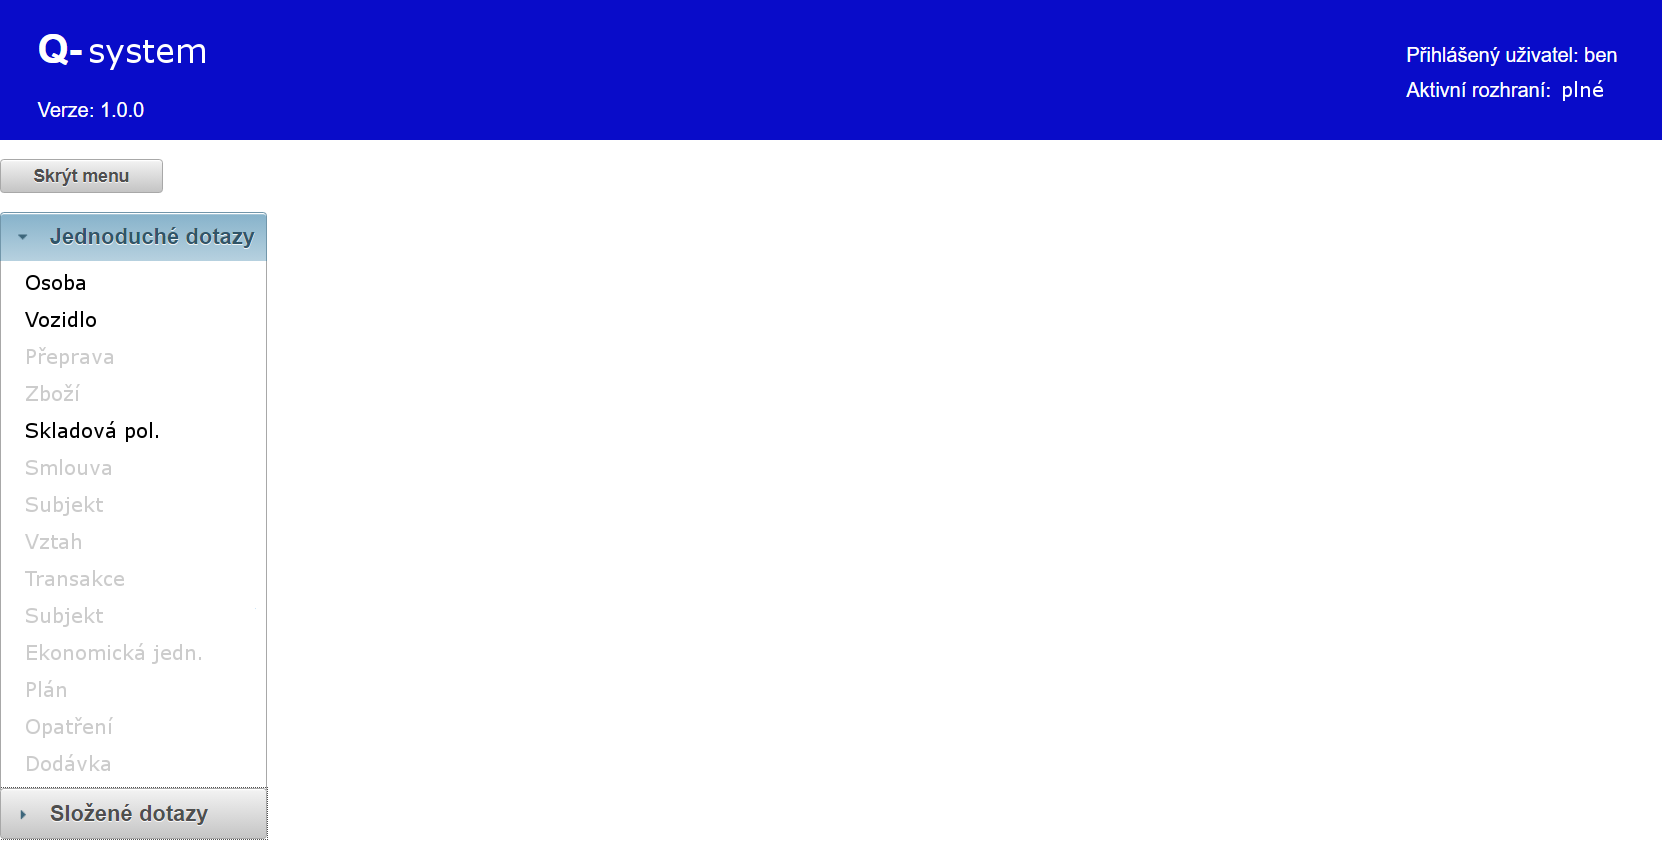
\includegraphics[width=\textwidth]{res/guide/Dashboard.png}
  \caption{Hlavní obrazovka}
  \label{fig:Hlavní obrazovka}
\end{figure}

V~záhlaví obrazovky je uveden název aplikace, její verze, informace o~přihlášeném uživateli a nastavení varianty rozhraní na IS~AAAA.

V~levé části obrazovky je menu aplikace, ve kterém jsou přístupné všechny funkce, které má přihlášený uživatel k~dispozici. Nad menu je tlačítko [Skrýt menu], pomocí kterého lze skrýt zobrazené menu. Pokud je menu skryté, je zde naopak tlačítko [Zobrazit menu] pro jeho opětovné zobrazení.

V~pravé části je pak prostor pro samotný obsah vybrané funkce – v~tomto prostoru uživatel definuje dotazy a pracuje s~jejich výsledky, případně řeší administrátorské úkony.

\subsubsection{Menu}
Menu je rozděleno do sekcí. Uživatel má přístupné vždy pouze sekce a funkce, pro která má nastavena oprávnění.

\newpage
\subsubsection{Ovládací prvky}
\label{OvladaciPrvky}
Funkce aplikace jsou ovládány následujícími prvky a postupy:

\begin{figure}[H]
  \centering
  
\includegraphics[scale=0.5]{res/guide/Button.png}
  \caption{Tlačítko}
  \label{fig:Tlačítko}
\end{figure}

\begin{figure}[H]
  \centering
  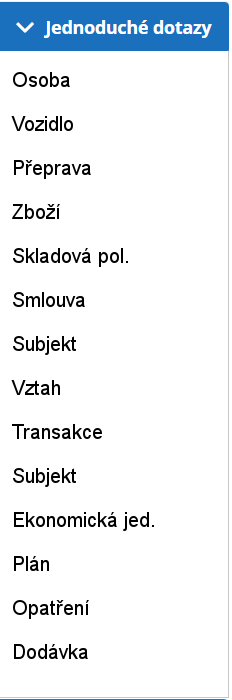
\includegraphics[scale=0.5]{res/guide/Menu.png}
  \caption{Menu}
  \label{fig:Menu}
\end{figure}

\begin{figure}[H]
  \centering
  
\includegraphics[scale=0.5]{res/guide/TextBox.png}
  \caption{Vstupní textové pole}
  \label{fig:Vstupní textové pole}
\end{figure}

\begin{figure}[H]
  \centering
  
\includegraphics[scale=0.5]{res/guide/ComboBox.png}
  \caption{Rozbalovací nabídka (\textit{combo-box})}
  \label{fig:Rozbalovací nabídka (combo-box)}
\end{figure}

\begin{figure}[H]
  \centering
  
\includegraphics[scale=0.5]{res/guide/CheckBox.png}
  \caption{Zaškrtávací pole (\textit{checkbox})}
  \label{fig:Zaškrtávací pole (checkbox)}
\end{figure}

\lbparagraph{Souborový dialog}

Pro výběr souboru se používá standardní dialog systému.

\newpage
\subsection{Spuštění a ukončení aplikace}
V~této kapitole je popsáno, jak aplikaci spustit, jak se do ní přihlásit a jak ji lze ukončit.

\subsubsection{Spuštění aplikace}
Aplikace se spouští vložením URL \url{http://localhost:8080} do internetového prohlížeče.

\subsubsection{Přihlášení}
\begin{figure}[H]
  \centering
  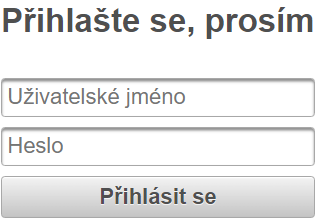
\includegraphics[scale=0.75]{res/guide/Login.png}
  \caption{Přihlašovací obrazovka}
  \label{fig:Přihlašovací obrazovka}
\end{figure}

Po načtení aplikace následuje ověření identity uživatele. Přihlašte se zadáním vašeho uživatelského jména a hesla. Přihlašovací údaje jsou shodné s~údaji do ostatních interních systémů vaší organizace, které se rovněž autentizují vůči Active Directory.

\subsubsection{Ukončení aplikace}
Aplikaci ukončíte zavřením příslušné záložky internetového prohlížeče, případně zavřením celého prohlížeče.

\subsection{Vkládání dat}
Pro vkládání dat slouží ovládací prvky popsané v~kapitole \hyperref[OvladaciPrvky]{Ovládací prvky}
\begin{itemize}
	\item Vstupní textové pole
	\item Combo-box
	\item Check-box
	\item Souborový dialog
\end{itemize}

\subsection{Chybová hlášení}
V~aplikaci se rozlišuje několik typů chyb podle jejich dopadu na práci uživatele:
\begin{itemize}
	\item Chyby vratné – aplikace zobrazí chybové hlášení, po jehož zavření zůstává ve stavu, ze kterého byla vyvolána (např. stiskem určitého tlačítka). Uživatel pak může provést úpravy a akci opakovat
	\item Chyby nevratné – aplikace zobrazí chybové hlášení, po jehož zavření se aplikace vrací před prováděnou akci (např. zavře okno, ve kterém chyba nastala, stejně, jako by ho zavřel uživatel tlačítkem [Zrušit])
\end{itemize}

\section{Popis funkcí}
Tato kapitola popisuje jednotlivé funkce aplikace, tj. dává návod, jak použít aplikaci jako podporu pro dosažení určitého cíle. Kapitola dává odpověď na otázku: \uv{Jak to mám udělat?}

\subsection{Popis funkcí pro uživatelskou roli Dotazovatel}
Funkce Dotazovatele souvisí s~pokládáním dotazů do IS~AAAA a s~následnou prací se zobrazeným výsledkem dotazu.

\subsubsection{Sestavit, odeslat dotaz a zobrazit jeho výsledek}
\lbparagraph{Účel funkce}
Funkce slouží k~sestavení požadovaného dotazu a k~jeho odeslání. Cílem je zobrazení výsledku takového dotazu.

\lbparagraph{Detailní popis funkce}
Uživatel si nejprve v~menu vybere typ dotazu, který chce položit. Následně v~zobrazených vyhledávacích kritériích zadá hledané hodnoty. Po odeslání dotazu aplikace dotaz do IS~AAAA provede a zobrazí jeho výsledek. Výsledkem je seznam nalezených záznamů. Uživatel si může zobrazit detail libovolného záznamu z~tohoto seznamu, a pokud jsou pro záznam dostupné i doplňkové údaje, tak si je může stáhnout pomocí doplňkového dotazu.

\lbparagraph{Navigace}
Nový dotaz lze položit z~libovolného místa aplikace použitím příslušné volby v~menu.

\lbparagraph{Popis jednotlivých kroků}

Použijte požadovaný typ dotazu v~menu. Typy dotazu jsou rozděleny na jednoduché dotazy (\textit{Single Category}) a složené dotazy (\textit{Multi Category}).

\begin{figure}[H]
  \centering
  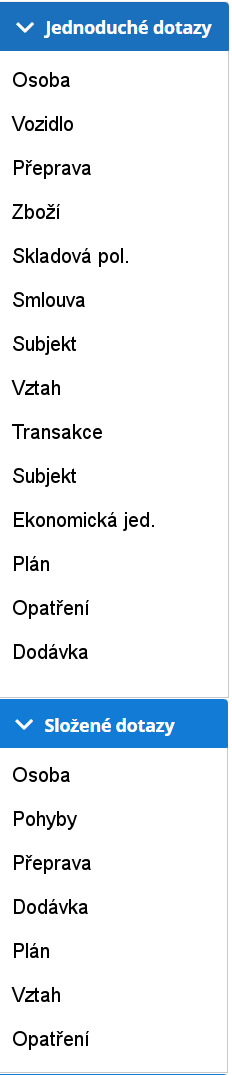
\includegraphics[scale=0.5]{res/guide/MenuFull.png}
  \caption{Celé menu}
  \label{fig:Celé menu}
\end{figure}

Aplikace zobrazí obrazovku pro zadání vyhledávacích kritérií pro vybraný typ dotazu.

\begin{figure}[H]
  \centering
  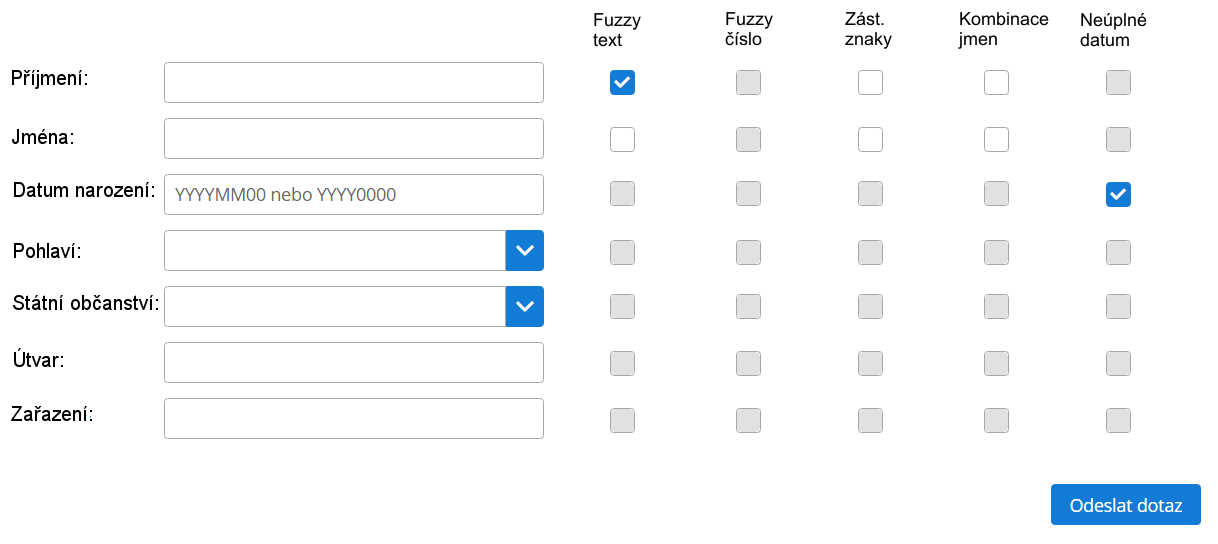
\includegraphics[width=\textwidth]{res/guide/SearchCriteria.png}
  \caption{Obrazovka s~vyhledávacími kritérii}
  \label{fig:ObrazovkaSVyhledavacimiKriterii}
\end{figure}

Zadejte hledané hodnoty do vstupních polí nebo je vyberte z~nabídky hodnot (\textit{combo-boxu}). U~každého pole je zobrazen seznam modifikátorů, přičemž některé mohou být nepřístupné (z~logiky věci nebo omezeny konfigurací systému). Zaškrtněte požadované modifikátory u~zadaných hledaných hodnot.

Odešlete připravený dotaz pomocí tlačítka [Odeslat dotaz].

Aplikace pod definicí dotazu zobrazí výsledek dotazu – seznam nalezených záznamů.

\begin{figure}[H]
  \centering
  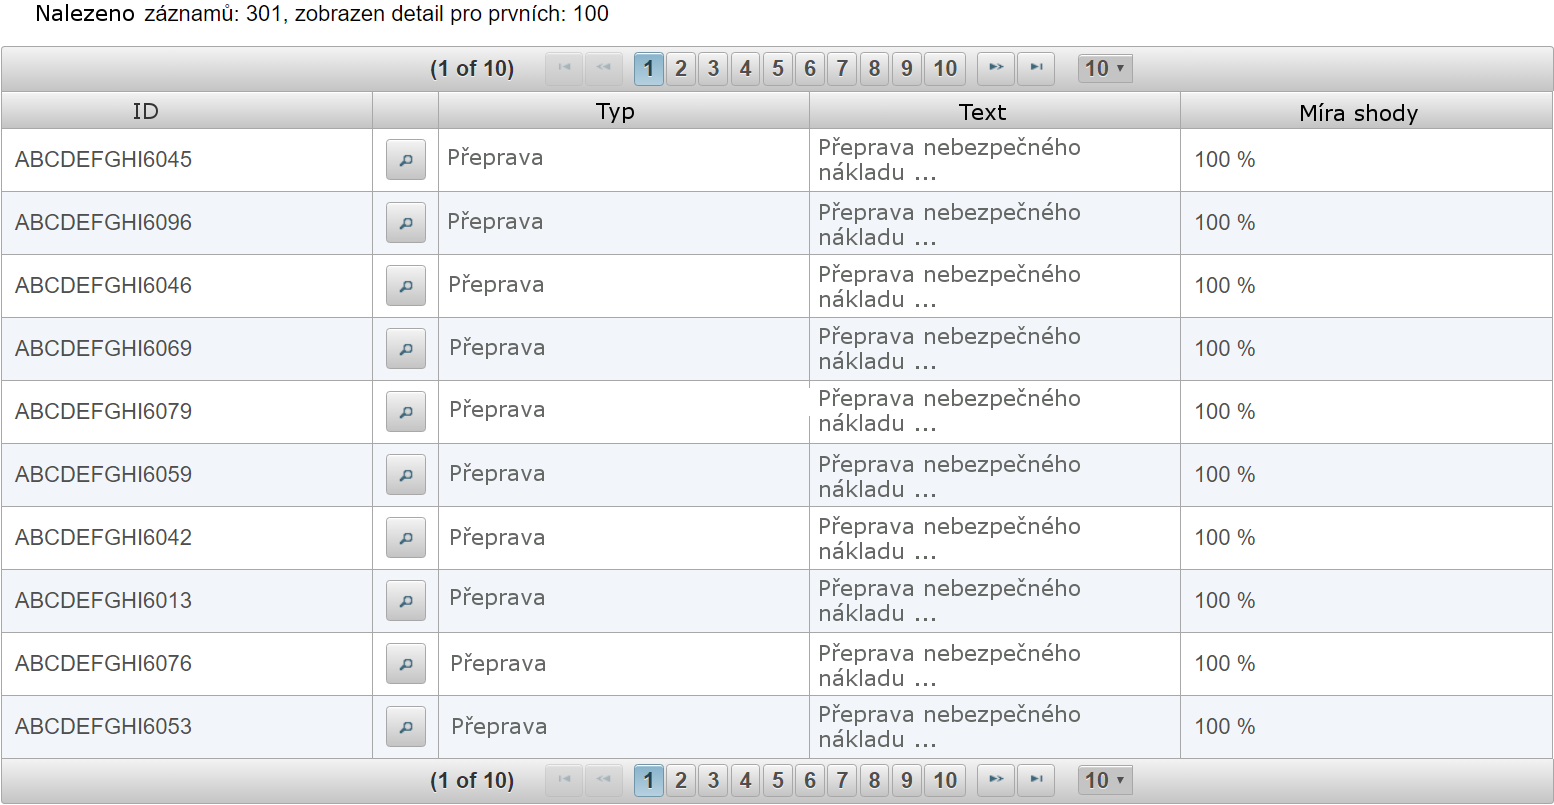
\includegraphics[width=\textwidth]{res/guide/ResponseData.png}
  \caption{Obrazovka se seznamem nalezených záznamů}
  \label{fig:Obrazovka se seznamem nalezených záznamů}
\end{figure}

Listujte v~seznamu nalezených záznamů pomocí navigační lišty (pro vysokou dostupnost je lišta k~dispozici v~horní i spodní části tabulky).

Obsah některých polí (hlavně sloupec \uv{Text}) může být poměrně rozsáhlý. Aby seznam nalezených záznamů zůstal přehledný, nezobrazuje se v~tabulce kompletní obsah, ale jen jeho fragment zakončený \uv{\ldots}. Kompletní obsah aplikace zobrazí při umístění myši nad dané pole v~\textit{tool-tipu}:
\begin{figure}[H]
  \centering
  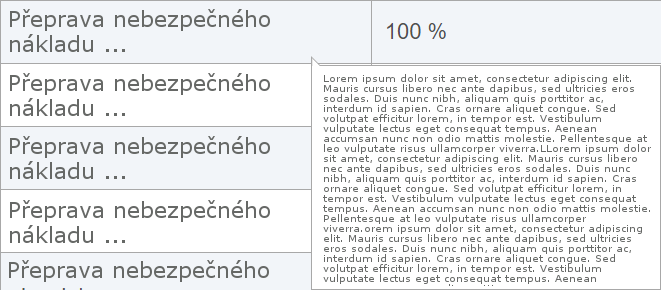
\includegraphics[scale=1.25]{res/guide/ResponseDataAction.png}
  \caption{Detail sloupce \uv{Text} ze záznamu}
  \label{fig:Detail sloupce Akce ze záznamu}
\end{figure}

Vyberte záznam a pomocí tlačítka 
\includegraphics[height=1em]{res/guide/SearchIcon.png} si zobrazte jeho detail.

Aplikace zobrazí detailní informace vybraného záznamu.

\begin{figure}[H]
  \centering
  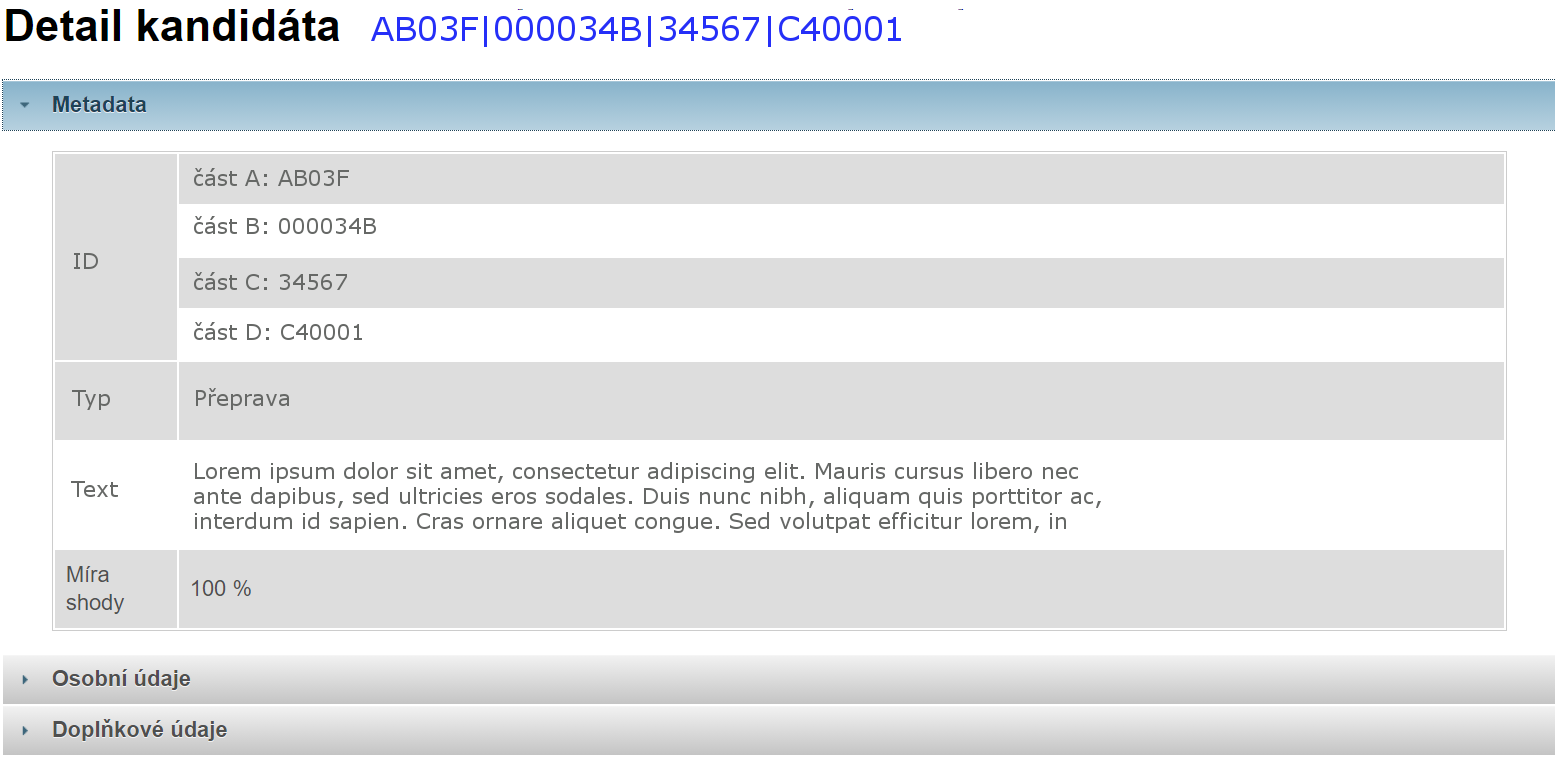
\includegraphics[width=\textwidth]{res/guide/ResponseDataDetail.png}
  \caption{Obrazovka s~detailem záznamu}
  \label{fig:Obrazovka s~detailem záznamu}
\end{figure}

Informace jsou rozděleny do logických sekcí, které lze rozbalovat a sbalovat (zde např. je rozbalena sekce \uv{Metadata} a sbalena sekce \uv{Osobní údaje}).

Pokud k~záznamu existuje doplňkový údaj a není zobrazen automaticky, zobrazte si jej pomocí tlačítka 
\includegraphics[height=1em]{res/guide/SearchIcon.png} u~tohoto údaje.

Aplikace zobrazí požadovaný údaj.

Pokud doplňkový údaj není vhodný pro okamžité zobrazení, uložte si soubor s~tímto údajem pomocí tlačítka 
\includegraphics[height=1em]{res/guide/SaveIcon.png}. Aplikace stáhne soubor s~tímto údajem a uloží do standardní systémové složky.

\subsection{Popis funkcí pro uživatelskou roli Administrátor}
Funkce Administrátora slouží k~nastavení chování systému. Do jeho kompetencí spadá správa dostupných forem dotazu a jejich přiřazování uživatelským rolím. Dále se stará o~parametry systému a udržování aktuálních číselníků.

\newpage
\subsubsection{Definovat novou formu dotazu}
\lbparagraph{Účel funkce}
Funkce slouží k~definici nové formy dotazu do IS~AAAA.

\lbparagraph{Detailní popis funkce}
Uživatel může definovat libovolnou sadu forem dotazů, které pak standardní uživatelé budou používat pro pokládání dotazů do IS~AAAA. Forma dotazu je tvořena sadou typů dotazu, sadou typů entit a nastavením jejich povolených modifikátorů. Jednotlivé formy dotazu se následně přidělují uživatelským rolím.

\lbparagraph{Navigace}
Založení nové formy dotazu lze zahájit z~libovolného místa aplikace použitím příslušné volby v~menu.

\lbparagraph{Popis jednotlivých kroků}
Použijte v~menu v~sekci \uv{Administrace} volbu Formy dotazu.
Aplikace zobrazí seznam existujících forem dotazu.

\begin{figure}[H]
  \centering
  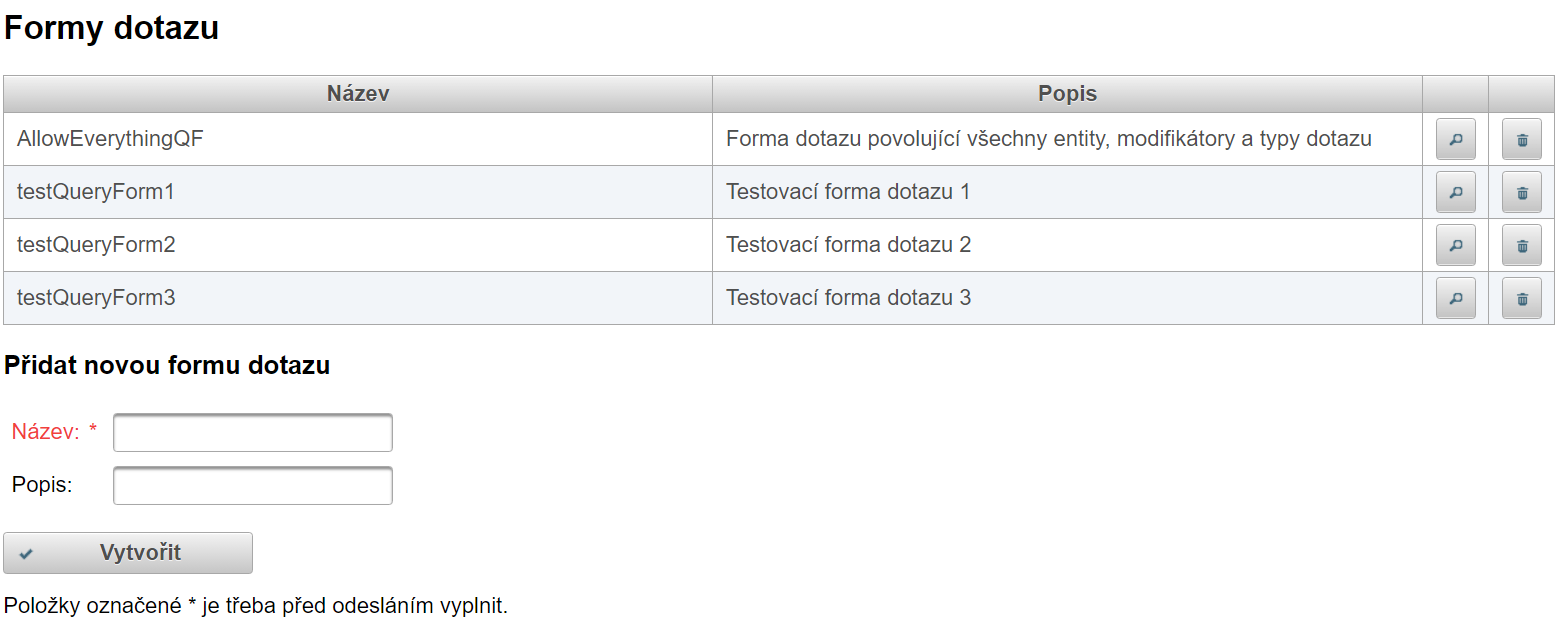
\includegraphics[width=\textwidth]{res/guide/QueryForms.png}
  \caption{Obrazovka s~administrací forem dotazu}
  \label{fig:Obrazovka s~administrací forem dotazu}
\end{figure}

Vyplňte pole \uv{Název} a \uv{Popis} v~části \uv{Přidat novou formu dotazu} a potvrďte zadané údaje tlačítkem [Vytvořit].

Aplikace přidá novou formu dotazu do seznamu.

Použijte tlačítko 
\includegraphics[height=1em]{res/guide/SearchIcon.png} u~vytvořené formy dotazu.
 
Aplikace zobrazí obrazovku pro definici formy dotazu.

\begin{figure}[H]
  \centering
  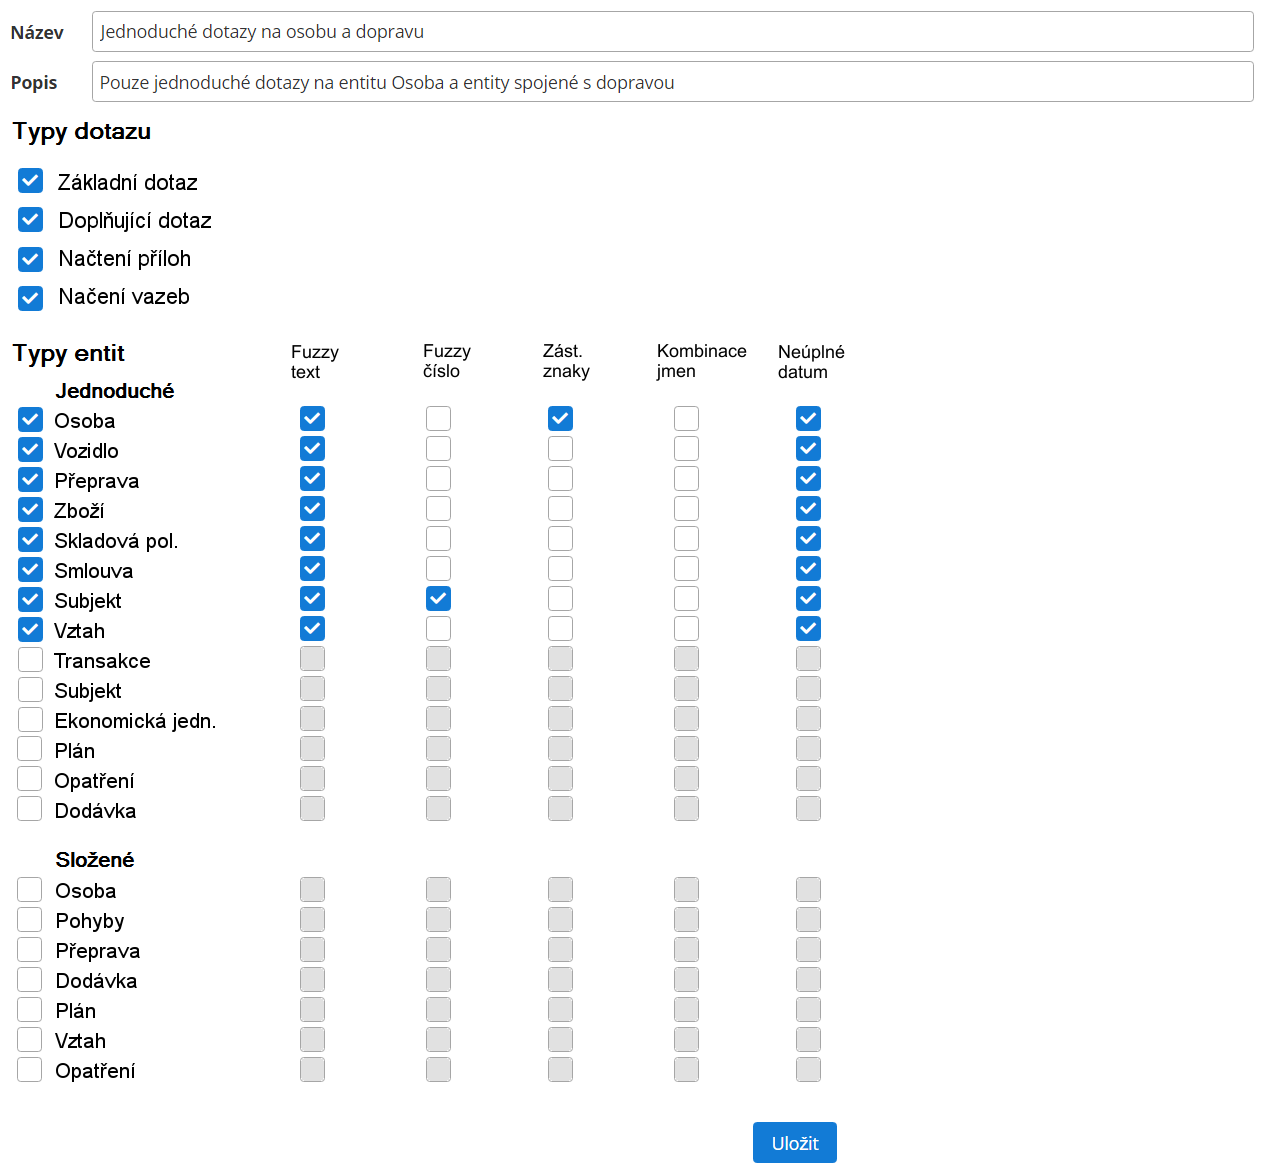
\includegraphics[width=\textwidth]{res/guide/QueryFormDetail.png}
  \caption{Obrazovka s~detailem konkrétní formy dotazu}
  \label{fig:Obrazovka s~detailem konkrétní formy dotazu}
\end{figure}

Vyberte typy dotazu, které bude tato forma dotazu povolovat.

Vyberte entity, na které bude možné pokládat dotazy a modifikátory, které se budou moci v~dotazech používat.

Potvrďte definici formy dotazu pomocí tlačítka [Uložit].

Aplikace založí novou formu dotazu a zobrazí seznam všech forem dotazu.

\textbf{Alternativně:} Vraťte se na seznam forem dotazu bez uložení změn pomocí volby \uv{Zpět na výpis} v~horní části obrazovky.

\newpage
\subsubsection{Upravit existující formu dotazu}
\lbparagraph{Účel funkce}
Funkce slouží ke změně definice existující formy dotazu do IS~AAAA.

\lbparagraph{Detailní popis funkce}
Uživatel může upravit libovolnou existující formu dotazu. Úprava je identická s~definicí nové formy.

\lbparagraph{Navigace}
Editaci formy dotazu lze zahájit z~libovolného místa aplikace použitím příslušné volby v~menu.

\lbparagraph{Popis jednotlivých kroků}
Použijte v~menu v~sekci \uv{Administrace} volbu Formy dotazu.

Aplikace zobrazí seznam existujících forem dotazu.

\begin{reusefigure}[H]{fig:Obrazovka s~administrací forem dotazu}
  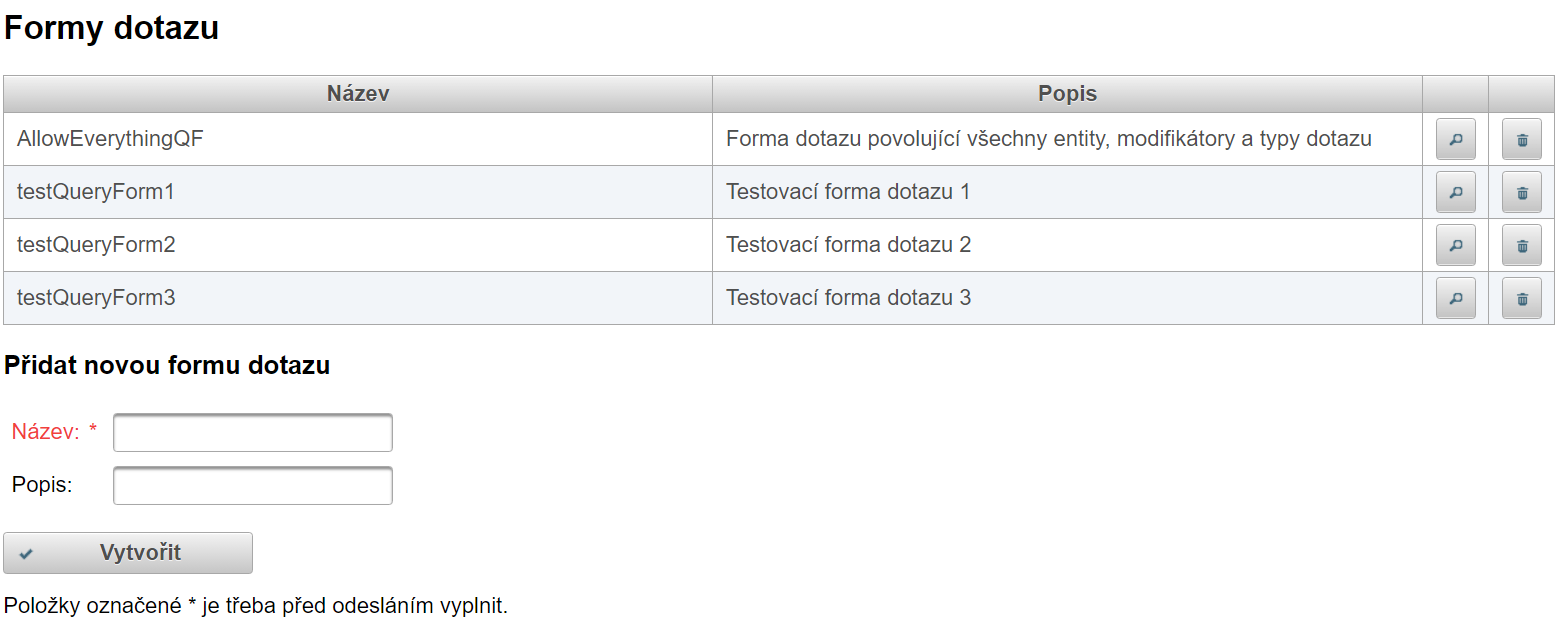
\includegraphics[width=\textwidth]{res/guide/QueryForms.png}
  \caption{Obrazovka s~administrací forem dotazu}
\end{reusefigure}

Vyberte existující formu dotazu a pomocí tlačítka 
\includegraphics[height=1em]{res/guide/SearchIcon.png} si zobrazte její detail.
Aplikace zobrazí obrazovku s~definicí vybrané formy dotazu.

\begin{reusefigure}[H]{fig:Obrazovka s~detailem konkrétní formy dotazu}
  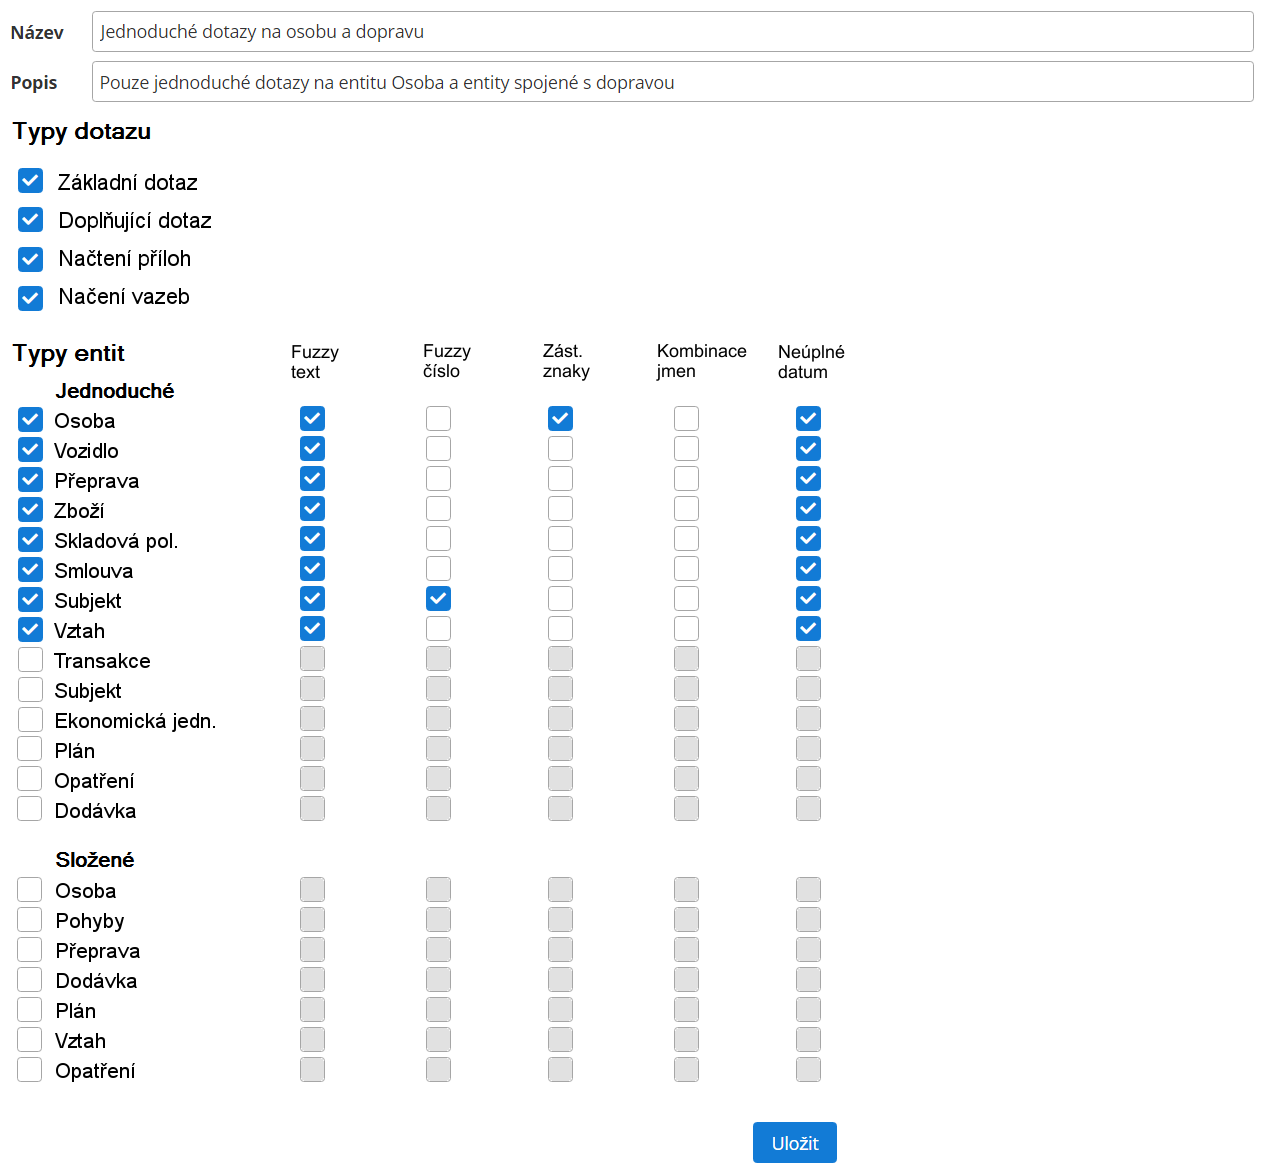
\includegraphics[width=\textwidth]{res/guide/QueryFormDetail.png}
  \caption{Obrazovka s~detailem konkrétní formy dotazu}
\end{reusefigure}

Vyberte typy dotazu, které bude tato forma dotazu povolovat.

Vyberte entity, na které bude možné pokládat dotazy a modifikátory, které se budou moci v~dotazech používat.

Potvrďte definici formy dotazu pomocí tlačítka [Uložit].

Aplikace založí novou formu dotazu a zobrazí seznam všech forem dotazu.

\textbf{Alternativně:} Vraťte se na seznam forem dotazu bez uložení změn pomocí volby \uv{Zpět na výpis} v~horní části obrazovky.

\newpage
\subsubsection{Zrušit existující formu dotazu}
\lbparagraph{Účel funkce}
Funkce slouží ke zrušení existující formy dotazu do IS~AAAA.

\lbparagraph{Detailní popis funkce}
Uživatel může zrušit libovolnou existující formu dotazu. Forma dotazu je po zrušení automaticky odstraněna od uživatelských rolí, ke kterým byla přiřazena.

\lbparagraph{Navigace}
Zrušení formy dotazu lze zahájit z~libovolného místa aplikace použitím příslušné volby v~menu.

\lbparagraph{Popis jednotlivých kroků}
Použijte v~menu v~sekci \uv{Administrace} volbu Formy dotazu.
Aplikace zobrazí seznam existujících forem dotazu.

\begin{reusefigure}[H]{fig:Obrazovka s~administrací forem dotazu}
  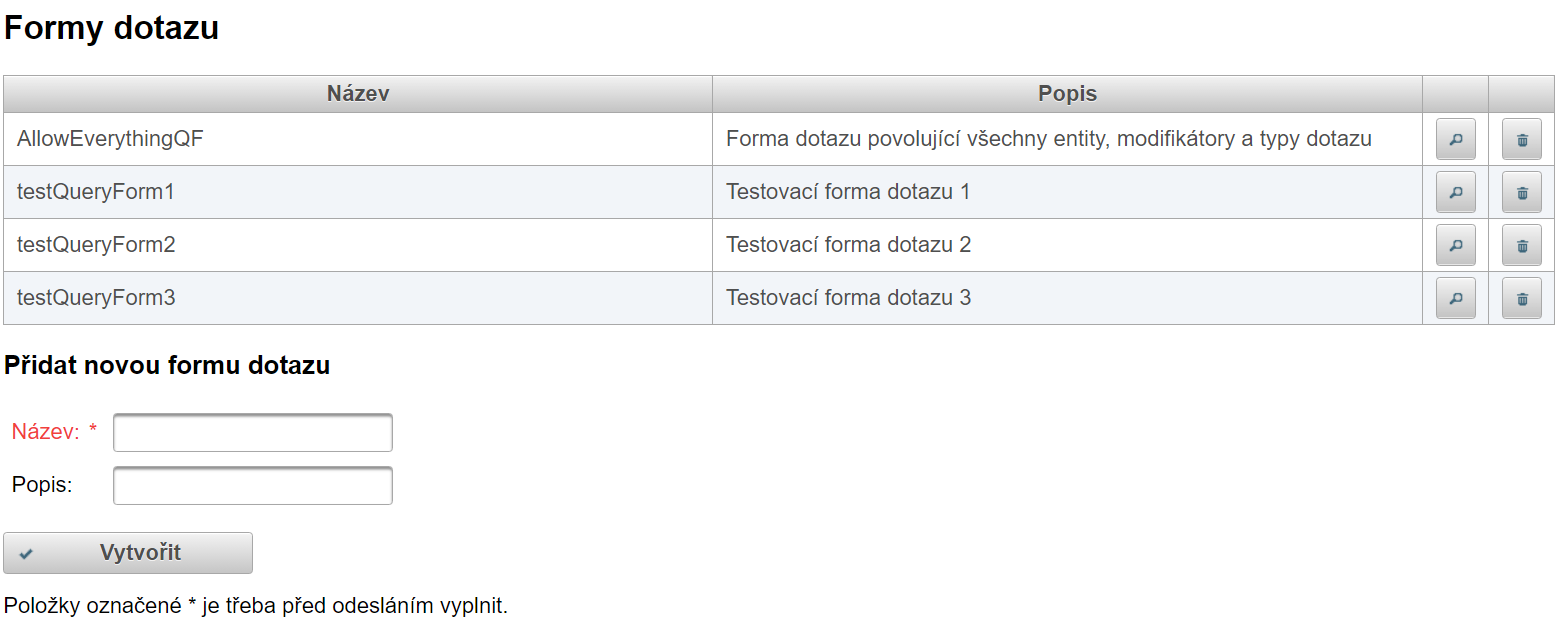
\includegraphics[width=\textwidth]{res/guide/QueryForms.png}
  \caption{Obrazovka s~administrací forem dotazu}
\end{reusefigure}

Vyberte existující formu dotazu a pomocí tlačítka 
\includegraphics[height=1em]{res/guide/RemoveIcon.png} ji zrušte.

Aplikace zobrazí potvrzovací dotaz, který potvrďte. 

\begin{figure}[H]
  \centering
  
\includegraphics[scale=0.5]{res/guide/ConfirmationDialog.png}
  \caption{Potvrzovací dialogové okno}
  \label{fig:Potvrzovací dialogové okno}
\end{figure}

Aplikace následně odstraní formu dotazu a zobrazí aktuální seznam forem dotazu.

\subsubsection{Definovat novou uživatelskou roli}
\lbparagraph{Účel funkce}
Funkce slouží k~definici nové uživatelské role.

\lbparagraph{Detailní popis funkce}
Uživatel může definovat libovolnou sadu uživatelských rolí. Uživatelské role jsou pomocí Active Directory přiřazovány uživatelům. Uživatelská role představuje určitý předpis, jakým způsobem může s~aplikací pracovat libovolný uživatel, který má tuto roli přiřazenou. Předpis uživatelské role spočívá v~definici, jaké formy dotazu může používat.

\lbparagraph{Navigace}
Založení nové uživatelské role lze zahájit z~libovolného místa aplikace použitím příslušné volby v~menu.

\lbparagraph{Popis jednotlivých kroků}
Použijte v~menu v~sekci \uv{Administrace} volbu Uživatelské role.

Aplikace zobrazí seznam existujících uživatelských rolí.

\begin{figure}[H]
  \centering
  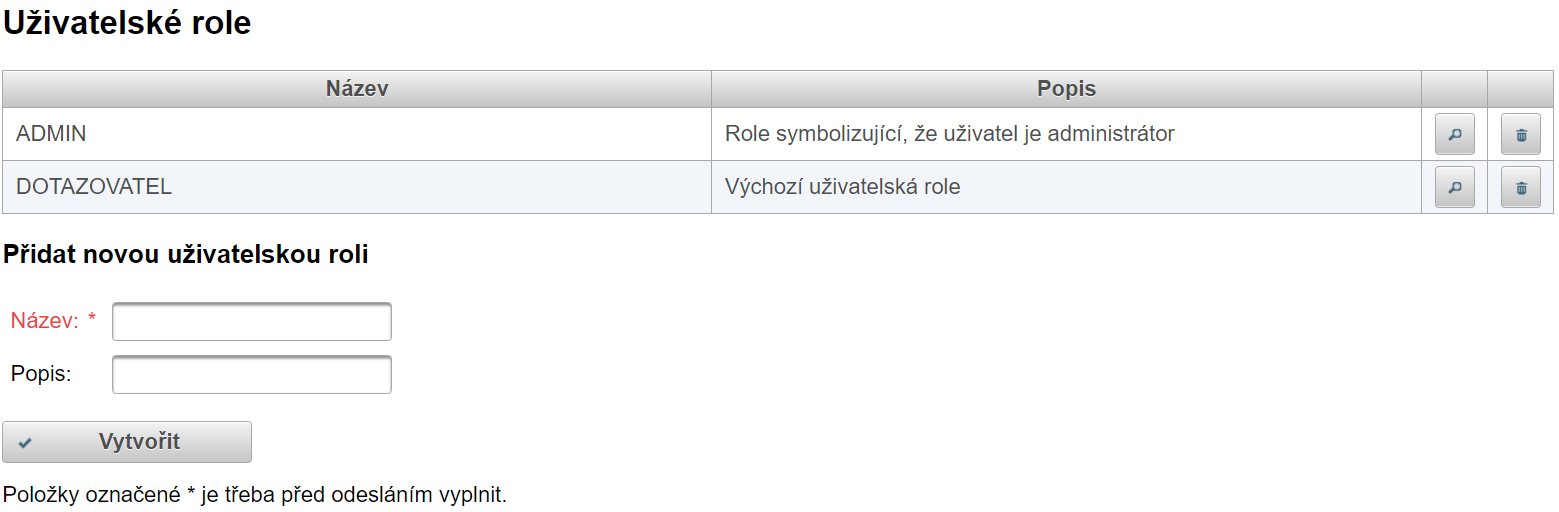
\includegraphics[width=\textwidth]{res/guide/UserRoles.png}
  \caption{Obrazovka s~administrací uživatelských rolí}
  \label{fig:Obrazovka s~administrací uživatelských rolí}
\end{figure}

Vyplňte pole \uv{Název} (musí být unikátní) a \uv{Popis} v~části \uv{Přidat novou uživatelskou roli} a potvrďte zadané údaje tlačítkem [Vytvořit].

Aplikace vytvoří novou roli a zobrazí ji v~seznamu rolí.

Otevřete definici nově vytvořené role pomocí tlačítka 
\includegraphics[height=1em]{res/guide/SearchIcon.png}.

Aplikace zobrazí obrazovku pro definici uživatelské role.

\begin{figure}[H]
  \centering
  \includegraphics[scale=0.60]{res/guide/UserRoleDetail.png}
  \caption{Obrazovka s~detailem konkrétní uživatelské role}
  \label{fig:Obrazovka s~detailem konkrétní uživatelské role}
\end{figure}

Vyberte formy dotazu, které bude moci uživatel s~touto rolí používat.

Potvrďte definici uživatelské role pomocí tlačítka [Uložit].

Aplikace uloží definici role a zobrazí seznam všech uživatelských rolí.

\textbf{Alternativně:} Vraťte se na seznam uživatelských rolí bez uložení změn pomocí volby \uv{Zpět na výpis} v~horní části obrazovky.

\newpage
\subsubsection{Upravit existující uživatelskou roli}
\lbparagraph{Účel funkce}
Funkce slouží ke změně definice existující uživatelské role.

\lbparagraph{Detailní popis funkce}
Uživatel může upravit libovolnou existující uživatelskou roli. Úprava je identická s~definicí nové role.

\lbparagraph{Navigace}
Editaci uživatelské role lze zahájit z~libovolného místa aplikace použitím příslušné volby v~menu.

\lbparagraph{Popis jednotlivých kroků}
Použijte menu v~sekci \uv{Administrace} volbu Uživatelské role.

Aplikace zobrazí seznam existujících uživatelských rolí.

\begin{reusefigure}[H]{fig:Obrazovka s~administrací uživatelských rolí}
  \includegraphics[width=\textwidth]{res/guide/UserRoles.png}
  \caption{Obrazovka s~administrací uživatelských rolí}
\end{reusefigure}

Vyberte existující roli a pomocí tlačítka \includegraphics[height=1em]{res/guide/SearchIcon.png} si zobrazte její detail.
Aplikace zobrazí obrazovku s~definicí vybrané uživatelské role.

\begin{reusefigure}[H]{fig:Obrazovka s~detailem konkrétní uživatelské role}
  \centering
  \includegraphics[scale=0.60]{res/guide/UserRoleDetail.png}
  \caption{Obrazovka s~detailem konkrétní uživatelské role}
\end{reusefigure}

Vyberte formy dotazu, které bude moci uživatel s~touto rolí používat.

Potvrďte definici uživatelské role pomocí tlačítka [Uložit].

Aplikace uloží upravenou uživatelskou roli a zobrazí seznam všech uživatelských rolí.

\textbf{Alternativně:} Vraťte se na seznam uživatelských rolí bez uložení změn pomocí volby \uv{Zpět na výpis} v~horní části obrazovky.

\newpage
\subsubsection{Zrušit existující uživatelskou roli}
\lbparagraph{Účel funkce}
Funkce slouží ke zrušení existující uživatelské role.

\lbparagraph{Detailní popis funkce}
Uživatel může zrušit libovolnou existující uživatelskou roli. Odstranění role z~Active Directory je třeba učinit samostatně.

\lbparagraph{Navigace}
Zrušení uživatelské role lze zahájit z~libovolného místa aplikace použitím příslušné volby v~menu.

\lbparagraph{Popis jednotlivých kroků}
Použijte v~menu v~sekci \uv{Administrace} volbu Uživatelské role.

Aplikace zobrazí seznam existujících uživatelských rolí.

\begin{reusefigure}[H]{fig:Obrazovka s~administrací uživatelských rolí}
  \includegraphics[width=\textwidth]{res/guide/UserRoles.png}
  \caption{Obrazovka s~administrací uživatelských rolí}
\end{reusefigure}

Vyberte existující roli a pomocí tlačítka \includegraphics[height=1em]{res/guide/RemoveIcon.png} ji zrušte.

Aplikace zobrazí potvrzovací dotaz, který potvrďte. 

\begin{reusefigure}[H]{fig:Potvrzovací dialogové okno}
  \centering
  \includegraphics[scale=0.5]{res/guide/ConfirmationDialog.png}
  \caption{Potvrzovací dialogové okno}
\end{reusefigure}

Aplikace následně odstraní uživatelskou roli a zobrazí aktuální seznam uživatelských rolí.

\newpage
\subsubsection{Aktualizovat překladové číselníky}
\lbparagraph{Účel funkce}
Funkce slouží k~aktualizaci překladových číselníků používaných ve vyhledávacích kritériích dotazů.

\lbparagraph{Detailní popis funkce}
Pomocí této funkce Administrátor nahraje do systému aktuální hodnoty překladových číselníků. Aplikace tyto číselníky používá v~nabídkách (\textit{combo-boxech}) vyhledávacích kritériích při přípravě dotazu.

\lbparagraph{Navigace}
Aktualizaci překladových číselníků lze zahájit z~libovolného místa aplikace použitím příslušné volby v~menu.

\lbparagraph{Popis jednotlivých kroků}
Použijte v~menu v~sekci \uv{Administrace} volbu Překladové číselníky.

Aplikace zobrazí obrazovku s~údajem o~poslední aktualizaci.

\begin{figure}[H]
  \centering
  \includegraphics[width=\textwidth]{res/guide/TranslationDials.png}
  \caption{Souborový dialog pro nahrání překladových číselníků}
  \label{fig:Souborový dialog pro nahrání překladových číselníků}
\end{figure}

Vyberte TOML soubor s~aktuálními hodnotami číselníků a volbu potvrďte.

Aplikace provede aktualizaci a zobrazí její výsledek.

\newpage
\subsubsection{Nastavit preferované rozhraní na IS~AAAA}
\lbparagraph{Účel funkce}
Funkce slouží k~nastavení preferovaného rozhraní na IS~AAAA.

\lbparagraph{Detailní popis funkce}
Preferované rozhraní je takové, které se má standardně používat. Pokud je toto rozhraní nedostupné, aplikace se pokusí přepnout na druhé rozhraní.
Pracuje se pouze se dvěma rozhraními – \textit{Plné rozhraní} a \textit{Zjednodušené rozhraní}.

\lbparagraph{Navigace}
Nastavení preferovaného rozhraní lze zahájit z~libovolného místa aplikace použitím příslušné volby v~menu.

\lbparagraph{Popis jednotlivých kroků}
Použijte v~menu v~sekci \uv{Administrace} volbu Rozhraní na IS~AAAA.
Aplikace zobrazí údaje o~preferovaném a aktuálně používaném rozhraní.

\begin{figure}[H]
  \centering
  \includegraphics[width=\textwidth]{res/guide/InterfaceSelection.png}
  \caption{Obrazovka s~informacemi o~rozhraní IS~AAAA}
  \label{fig:Obrazovka s~informacemi o~rozhraní IS~AAAA}
\end{figure}

Použijte tlačítko [Změnit].

Aplikace zobrazí okno pro výběr rozhraní.

\begin{figure}[H]
  \centering
  \includegraphics[scale=0.75]{res/guide/InterfaceSelectionSwitch.png}
  \caption{Obrazovka výběrem z~rozhraní IS~AAAA}
  \label{fig:Obrazovka výběrem z~rozhraní IS~AAAA}
\end{figure}

Vyberte preferované rozhraní a volbu potvrďte tlačítkem [Uložit].

Aplikace zobrazí aktualizované informace o~preferovaném rozhraní.

\newpage
\subsubsection{Nastavit používané rozhraní na preferované}
\lbparagraph{Účel funkce}
Funkce slouží k~nastavení aktuálně používaného rozhraní na preferované.

\lbparagraph{Detailní popis funkce}
Pomocí této funkce lze rovněž změnit preferované rozhraní, nikoliv ovšem výběrem z~více možností, ale jako preferované bude nastavené aktuálně používané rozhraní.

\lbparagraph{Navigace}
Nastavení na preferované rozhraní lze zahájit z~libovolného místa aplikace použitím příslušné volby v~menu.

\lbparagraph{Popis jednotlivých kroků}
Použijte v~menu v~sekci \uv{Administrace} volbu Rozhraní na IS~AAAA.

Aplikace zobrazí údaje o~preferovaném a aktuálně používaném rozhraní.

\begin{reusefigure}[H]{fig:Obrazovka s~informacemi o~rozhraní IS~AAAA}
  \includegraphics[width=\textwidth]{res/guide/InterfaceSelection.png}
  \caption{Obrazovka s~informacemi o~rozhraní IS~AAAA}
\end{reusefigure}

Použijte tlačítko [Nastavit na preferované].

Aplikace nastaví aktuálně používané rozhraní na preferované a aktualizuje zobrazené údaje.

\begin{conclusion}
Zadavatel si přál omezit nevhodné pokládání dotazů do Informačního systému AAA a zároveň vlastnit vzorový dotazovací systém, který by bylo možné poskytnout menším organizacím, ať už pouze jako referenční systém umoňující pokládat pouze validní dotazy, nebo jako základ pro vybudování vlastního dotazovacího systému.

Mnou navrženým vzorovým dotazovacím systémem pro Informační systém AAA se mi podařilo toto přání naplnit. Prošel jsem si všemi částmi vývoje SW kulminující úspěšnou akceptací produktu zadavatelem. Díky tomu jsem získal nadhled a cenné zkušenosti mimo současné profesní zaměření -- programování.

Úspěšně jsem splnil stanovené cíle práce:
\begin{enumerate}
	\item Nastudoval jsem širokou škálu nabízené funkcionality IS~AAA. Zkoumanou doménu a požadavky na systém jsem popsal v~analytické části práce -- \hyperref[Analyza]{\textit{Analýza}}.
	\item V~kapitole \hyperref[Navrh]{\textit{Návrh}} jsem za použití inženýrských postupů provedl návrh předmětného softwarového systému s~detailním popisem scénářů případů použití. V~návrhu jsem zohlednil všechny požadavky kladené na systém.
	\item Vytvořil jsem uživatelskou dokumentaci, která je obsažena v~kapitole\\ \hyperref[UzivatelskaPrirucka]{\textit{Uživatelská příručka}}.
	\item Implementační část jsem popsal kapitolou \hyperref[Realizace]{\textit{Realizace}}. Věnoval jsem velké usílí tvorbě kvalitního strukturovaného kódu, aby byl přehledný a snadno rozšiřitelný v~budoucnosti. Myslel jsem na správný design dle zásad softwarového inženýrství, samozřejmostí bylo vytvoření unit testů a také integračních testů. Jsem na výslednou podobu kódu opravdu hrdý a přebírám za něj plnou odpovědnost, také vůči zadavateli.
\end{enumerate}

\newpage 
Finálním cílem práce bylo pouze vytvoření funkčního prototypu backendové části aplikace, mně se ovšem navíc podařilo odevzdat celou funkční aplikaci. Podílel jsem se také na frontendové části aplikace. Transparentně jsem popsal, na jakých částech spolupracoval někdo z~mých kolegů. 

Mám radost z~toho, že výsledný produkt této diplomové práce je reálně využitelný, a jsem přesvědčen, že jsem při jeho návrhu a tvorbě prokázal svoji odbornou způsobilost odpovídající magisterskému studiu na Fakultě informačních techonolií Českého vysokého učení technického v~Praze. 
\end{conclusion}

%\renewcommand{\refname}{Seznam literatury}
%\newpage
\bibliographystyle{csn690}
\begin{thebibliography}{9}
	\bibitem{IsAAA}
	\textit{Popis systému IsAAA}. [interní dokument]. KOMIX s.r.o. 6/9/2017. [cit. 21/2/2020]
	
	\bibitem{ICT}
	\textit{Číselníky ICT}. [interní excelový dokument]. [cit. 21/2/2020]
	
	\bibitem{Queries}
	\textit{Queries Description}. [interní dokument]. [cit. 21/2/2020]
	
	\bibitem{i1}
	\textit{Popis rozhraní Plné rozhraní}. [interní dokument]. [cit. 21/2/2020]
		
	\bibitem{i2}
	\textit{Popis rozhraní Zjednodušené rozhraní}. [interní dokument]. [cit. 21/2/2020]

	\bibitem{FatJar}
	\textit{Create a Fat Jar App with Spring Boot} [online]. Baeldung. [cit. 2/3/2020]. Dostupné z: \url{https://www.baeldung.com/deployable-fat-jar-spring-boot}

	\bibitem{ApplicationServers}
	SALNIKOV-TARNOVSKI, Nikita. \textit{Most popular Java application servers: 2017 edition} [online]. Plumbr. 23/5/2017. [cit. 2/3/2020]. Dostupné z: \url{https://plumbr.io/blog/java/most-popular-java-application-servers-2017-edition}

	\bibitem{Tomcat}
	\textit{3 Difference between Web Server vs Application vs Servlet Containers in Java JEE} [online]. Java67. 2/6/2016. [cit. 2. 3. 2020]. Dostupné z: \url{https://www.java67.com/2016/06/3-difference-between-web-server-vs-application-server-vs-servlet-container.html}
	
	\bibitem{JavaHistory}
	\textit{Java version history} [online]. Wikipedia. [cit. 4. 3. 2020]. Dostupné z: \url{https://en.wikipedia.org/wiki/Java_version_history}
	
	\bibitem{OpenJDK}
	\textit{Archived OpenJDK General-Availability Releases} [online]. jdk.java.net. [cit. 4. 3. 2020]. Dostupné z: \url{https://jdk.java.net/archive/}	
	
	\bibitem{JSON}
	McCOMBS, Thayne. \textit{Why JSON isn’t a Good Configuration Language} [online]. Lucidchart. 16/6/2018. [cit. 4/3/2020]. Dostupné z: \url{https://www.lucidchart.com/techblog/2018/07/16/why-json-isnt-a-good-configuration-language}

	\bibitem{TOML}
PRESTON-WERNER, Tom. \textit{TOML} [online]. GitHub. [cit. 4/3/2020]. Dostupné z: \url{https://github.com/toml-lang/toml#toml}

	\bibitem{SPAvsMPA}
	\textit{Single-page application vs. multiple-page application} [online]. A~Medium Corporation. 2/12/2016. [cit. 5/3/2020]. Dostupné z: \url{https://medium.com/@NeotericEU/single-page-application-vs-multiple-page-application-2591588efe58}
	
	\bibitem{DontNeedSPA}
	\textit{You probably don't need a single-page application} [online]. The Plausible Journal. 29/1/2019. [cit. 5/3/2020]. Dostupné z: \url{https://journal.plausible.io/you-probably-dont-need-a-single-page-app}

	\bibitem{JSPvsJSF}
	\textit{Difference Between JSP vs JSF} [online]. Educba. [cit. 7/3/2020]. Dostupné z: \url{https://www.educba.com/jsp-vs-jsf}
	
	\bibitem{Primefaces}
	\textit{Prime faces} [online]. Primefaces.org. [cit. 7/3/2020]. Dostupné z: \url{https://www.
	.org/showcase}
	
	\bibitem{OpenSourceLicence}
	\textit{Licenses \& Standards} [online]. Open Source Initiative. [cit. 7/3/2020]. Dostupné z: \url{https://opensource.org/licenses}
	
	\bibitem{CodeNotFound}
	\textit{JSF PrimeFaces Example} [online]. CodeNotFound. 22/11/2018. [cit. 18/3/2020]. Dostupné z: \url{https://codenotfound.com/jsf-primefaces-example.html}
	
	\bibitem{ManagedBeans}
	\textit{Java EE 6 @javax.annotation.ManagedBean vs. @javax.inject.Named vs. @javax.faces.ManagedBean} [online]. stackoverflow. 16/8/2012. [cit. 18/3/2020]. Dostupné z: \url{https://stackoverflow.com/questions/11986847/java-ee-6-javax-annotation-managedbean-vs-javax-inject-named-vs-javax-faces/12012663#12012663}
	
	\bibitem{CDI}
	\textit{Java EE CDI bean scopes} [online]. Java Code Geeks. 9/4/2013 [cit. 18/3/2020]. Dostupné z: \url{https://www.javacodegeeks.com/2013/04/java-ee-cdi-bean-scopes.html}
	
	\bibitem{JSFDI}
	\textit{JSF - Managed Beans} [online]. tutorialspoint. [cit. 18/3/2020]. Dostupné z: \url{https://www.tutorialspoint.com/jsf/jsf_managed_beans}
	
	\bibitem{JoinFaces}
	\textit{JoinFaces Reference Guide} [online]. joinfaces.org. [cit. 18/3/2020]. Dostupné z: \url{https://docs.joinfaces.org/4.1.4/reference}
	
	\bibitem{InjectIntoSingletonBean}
	\textit{Injecting Prototype Beans into a Singleton Instance in Spring} [online]. Baeldung. 16/9/2019. [cit. 18/3/2020]. Dostupné z: \url{https://www.baeldung.com/spring-inject-prototype-bean-into-singleton}
	
	\bibitem{EliminateSwitch}
	\textit{Ways to eliminate switch in code} [online]. stackoverflow. 24/9/2008. [cit. 18/3/2020]. Dostupné z: \url{https://stackoverflow.com/questions/126409/ways-to-eliminate-switch-in-code}
	
	\bibitem{InheritanceVsComposition}
	\textit{Replacing Inheritance with Composition} [online]. Programming Ideas With Jake. [cit. 18/3/2020]. Dostupné z: \url{https://programmingideaswithjake.wordpress.com/2015/05/09/replacing-inheritance-with-composition}	
	
	\bibitem{JaxWS}
	\textit{Introduction to JAX-WS} [online]. Baeldung. 17/1/2019. [cit. 19/3/2020]. Dostupné z: \url{https://www.baeldung.com/jax-ws}		
	
	\bibitem{JAXB}
	GUPTA, Lokesh. \textit{JAXB – Marshal and Unmarshal List or Set of Objects} [online]. HowToDoInJava. [cit. 19/3/2020]. Dostupné z: \url{https://howtodoinjava.com/jaxb/jaxb-exmaple-marshalling-and-unmarshalling-list-or-set-of-objects}	
	
	\bibitem{DOMParser}
	GUPTA, Lokesh. \textit{Java Read XML – Java DOM Parser Example} [online]. HowToDoInJava. [cit. 19/3/2020]. Dostupné z: \url{https://howtodoinjava.com/xml/read-xml-dom-parser-example}
	
	\bibitem{ThreadSafety}
	UGARTE, Alejandro. \textit{What is Thread-Safety and How to Achieve it?} [online]. Baeldung. 7/12/2019. [cit. 19/3/2020]. Dostupné z: \url{https://www.baeldung.com/java-thread-safety}		
	
	\bibitem{JAXBThreadSafe}
	\textit{JAXB Frequently Asked Questions} [online]. Java EE Github. [cit. 19/3/2020]. Dostupné z: \url{https://javaee.github.io/jaxb-v2/doc/user-guide/ch06.html}		
	
	\bibitem{JaxWSThreadSafe}
	\textit{Annotation Type WebServiceRef} [online]. Java EE Oracle Documentation. [cit. 19/3/2020]. Dostupné z: \url{https://docs.oracle.com/javaee/6/api/javax/xml/ws/WebServiceRef.html}		
	
	\bibitem{KeyStore}
	\textit{Difference between trustStore vs keyStore in Java SSL} [online]. Java67. [cit. 20/3/2020]. Dostupné z: \url{https://www.java67.com/2012/12/difference-between-truststore-vs.html}		
	
	\bibitem{ApacheDS}
	\textit{ApacheDS v2.0 Basic User's Guide} [online]. The Apache Software Foundation. [cit. 20/3/2020]. Dostupné z: \url{https://directory.apache.org/apacheds/basic-user-guide.html}		
	
	\bibitem{SpringSecurity}
	\textit{Intro to Spring Security Expressions} [online]. Baeldung. 17/1/2020. [cit. 20/3/2020]. Dostupné z: \url{https://www.baeldung.com/spring-security-expressions}
\end{thebibliography}
%\bibliography{mybibliographyfile}

\appendix

\chapter{Seznam použitých zkratek a pojmů}
% \printglossaries
\begin{description}
	\item[API] Application Programming Interface
	\item[CDI] Contexts and Dependency Injection
	\item[CSS] Cascading Style Sheets
	\item[DI] Dependency Injection
	\item[EJB] Enterprise Java Beans
	\item[GUI] Graphical User Interface
	\item[HW] Computer Hardware
	\item[ISP] Interface Segregation Principle
	\item[JAXB] Java Architecture for XML Binding
	\item[JAX-WS] Java API for XML Web Services
	\item[JDK] Java Development Kit
	\item[JSF] Java Server Faces		
	\item[JSP] Java Server Pages
	\item[LDAP] Lightweight Directory Access Protocol
	\item[LTS] Long-Term Support
	\item[MPA] Multiple Page Application
	\item[MVC] Model View Controller	
	\item[OS] Operating System
	\item[QoS] Quality of service		
	\item[SEO] Search Engine Optimization
	\item[SOAP] Simple Object Access Protocol
	\item[SPA] Single Page Application
	\item[SSL] Secure Sockets Layer
	\item[SW] Computer Software
	\item[URL] Uniform Resource Locator
	\item[WSDL] Web Services Description Language
	\item[XHTML] EXtensible Hyper Text Markup Language
	\item[XLST] Extensible Stylesheet Language Transformations	
	\item[XML] Extensible Markup Language
	\item[XSD] XML Schema Definition
\end{description}

\chapter{Aktivity diagram pro položení dotazu}
Přikládám původní aktivity diagram, který jsem si vytvořil před popsáním scénářů případů užití. Diagram znázorňuje jednotlivé akce u~nejčastěji používaného procesu dotazovatele, tj. položení dotazu.

\begin{figure}[h]
  \centering
  \includegraphics[scale=0.29]{res/design/Activity diagram Položení dotazu.png}
  \caption{Aktivity diagram pro položení dotazu}
  \label{fig:Aktivity diagram pro položení dotazu}
\end{figure}


\chapter{Obsah přiloženého CD}
\begin{figure}
	\dirtree{%
		.1 qsystem\DTcomment{kopie repozitáře Q-systém}.
		.2 doc\DTcomment{programátorská dokumentace}.
		.2 qsystem-config\DTcomment{složka s~konfiguračními soubory Q-systému}.
		.2 qsystem-security\DTcomment{složka s~ukázkovými certifikáty}.
		.2 src\DTcomment{zdrojové soubory Q-systému}.
		.3 main.
		.4 java.
		.5 cz/komix/qsystem.
		.6 backend\DTcomment{backendová část aplikace}.
		.7 exception\DTcomment{vlastní výjimky}.
		.7 logic\DTcomment{aplikační vrstva}.
		.7 persistence\DTcomment{perzistentní vrstva}.
		.7 security\DTcomment{bezpečnost -- Spring security}.
		.7 service\DTcomment{servisní vrstva}.
		.6 frontend\DTcomment{frontendová část, kontrolery}.
		.4 resources.
		.5 app-features\DTcomment{popis nabízené funkcionality Q-systému}.
		.5 cz/komix/qsystem/frontend/messages\DTcomment{i18n textace}.
		.5 META-INF\DTcomment{frontendové šablony stránek}.
		.5 isaaa-interface-contract\DTcomment{XSD a WSDL}.
		.5 application.properties\DTcomment{Spring Boot property soubor}.
		.5 logback.xml\DTcomment{konfigurace logovacího frameworku Logback}.
		.3 test\DTcomment{integrační a unit testy}.
		.2 pom.xml\DTcomment{konfigurace Maven projektu}.
		.2 README.md\DTcomment{instalační příručka}.
		.1 thesis.
		.2 src.
		.3 DP\_Lejnar\_Jan\_2020.tex\DTcomment{text práce ve formátu \LaTeX{}}.
		.2 text.
		.3 DP\_Lejnar\_Jan\_2020.pdf\DTcomment{text práce ve formátu PDF}.
	}
\end{figure}

\end{document}
